

\documentclass[11pt,a4paper,twoside]{book}

\newcommand{\ficherosBasicosTeXiS}{%
TeXiS/TeXiS_pream,TeXiS/TeXiS_cab,TeXiS/TeXiS_bib,TeXiS/TeXiS_cover,%
TeXiS/TeXiS_part%
}
\newcommand{\compilaCapitulo}[1]{%
\includeonly{\ficherosBasicosTeXiS,\ficherosBasicosTexto,Capitulos/#1}%
}

\newcommand{\compilaApendice}[1]{%
\includeonly{\ficherosBasicosTeXiS,\ficherosBasicosTexto,Apendices/#1}%
}

%---------------------------------------------------------------------
%
%                          config.tex
%
%---------------------------------------------------------------------
%
% Contiene la  definici�n de constantes  que determinan el modo  en el
% que se compilar� el documento.
%
%---------------------------------------------------------------------
%
% En concreto, podemos  indicar si queremos "modo release",  en el que
% no  aparecer�n  los  comentarios  (creados  mediante  \com{Texto}  o
% \comp{Texto}) ni los "por  hacer" (creados mediante \todo{Texto}), y
% s� aparecer�n los �ndices. El modo "debug" (o mejor dicho en modo no
% "release" muestra los �ndices  (construirlos lleva tiempo y son poco
% �tiles  salvo  para   la  versi�n  final),  pero  s�   el  resto  de
% anotaciones.
%
% Si se compila con LaTeX (no  con pdflatex) en modo Debug, tambi�n se
% muestran en una esquina de cada p�gina las entradas (en el �ndice de
% palabras) que referencian  a dicha p�gina (consulta TeXiS_pream.tex,
% en la parte referente a show).
%
% El soporte para  el �ndice de palabras en  TeXiS es embrionario, por
% lo  que no  asumas que  esto funcionar�  correctamente.  Consulta la
% documentaci�n al respecto en TeXiS_pream.tex.
%
%
% Tambi�n  aqu� configuramos  si queremos  o  no que  se incluyan  los
% acr�nimos  en el  documento final  en la  versi�n release.  Para eso
% define (o no) la constante \acronimosEnRelease.
%
% Utilizando \compilaCapitulo{nombre}  podemos tambi�n especificar qu�
% cap�tulo(s) queremos que se compilen. Si no se pone nada, se compila
% el documento  completo.  Si se pone, por  ejemplo, 01Introduccion se
% compilar� �nicamente el fichero Capitulos/01Introduccion.tex
%
% Para compilar varios  cap�tulos, se separan sus nombres  con comas y
% no se ponen espacios de separaci�n.
%
% En realidad  la macro \compilaCapitulo  est� definida en  el fichero
% principal tesis.tex.
%
%---------------------------------------------------------------------


% Comentar la l�nea si no se compila en modo release.
% TeXiS har� el resto.
% ���Si cambias esto, haz un make clean antes de recompilar!!!
\def\release{1}


% Descomentar la linea si se quieren incluir los
% acr�nimos en modo release (en modo debug
% no se incluir�n nunca).
% ���Si cambias esto, haz un make clean antes de recompilar!!!
%\def\acronimosEnRelease{1}


% Descomentar la l�nea para establecer el cap�tulo que queremos
% compilar

% \compilaCapitulo{01Introduccion}
% \compilaCapitulo{02EstructuraYGeneracion}
% \compilaCapitulo{03Edicion}
% \compilaCapitulo{04Imagenes}
% \compilaCapitulo{05Bibliografia}
% \compilaCapitulo{06Makefile}

% \compilaApendice{01AsiSeHizo}

% Variable local para emacs, para  que encuentre el fichero maestro de
% compilaci�n y funcionen mejor algunas teclas r�pidas de AucTeX
%%%
%%% Local Variables:
%%% mode: latex
%%% TeX-master: "./Tesis.tex"
%%% End:


% Paquete de la plantilla
\usepackage{TeXiS/TeXiS}
\usepackage{wrapfig}
\usepackage{array}
\usepackage{float}
\restylefloat{table}
\usepackage{pgfplots}
\usepackage{amssymb}
\usepackage{tikz}
\usepackage{hyperref}
\hypersetup{
  citebordercolor=red,
  filebordercolor=red,
  linkbordercolor=red,
urlbordercolor=red
}
\urlstyle{same}

\usepackage{booktabs}
\usepackage{multirow}
\usepackage{adjustbox}
\usepackage{natbib}
\bibliographystyle{plainnat}


% Incluimos el fichero con comandos de constantes
%---------------------------------------------------------------------
%
%                          constantes.tex
%
%---------------------------------------------------------------------
%
% Fichero que  declara nuevos comandos LaTeX  sencillos realizados por
% comodidad en la escritura de determinadas palabras
%
%---------------------------------------------------------------------

%%%%%%%%%%%%%%%%%%%%%%%%%%%%%%%%%%%%%%%%%%%%%%%%%%%%%%%%%%%%%%%%%%%%%%
% Comando: 
%
%       \titulo
%
% Resultado: 
%
% Escribe el t�tulo del documento.
%%%%%%%%%%%%%%%%%%%%%%%%%%%%%%%%%%%%%%%%%%%%%%%%%%%%%%%%%%%%%%%%%%%%%%
\def\titulo{ Control Remoto de Videojuegos con Smartphones}

%%%%%%%%%%%%%%%%%%%%%%%%%%%%%%%%%%%%%%%%%%%%%%%%%%%%%%%%%%%%%%%%%%%%%%
% Comando: 
%
%       \autor
%
% Resultado: 
%
% Escribe el autor del documento.
%%%%%%%%%%%%%%%%%%%%%%%%%%%%%%%%%%%%%%%%%%%%%%%%%%%%%%%%%%%%%%%%%%%%%%
\def\autor{Pablo G\'omez Calvo y Sergio J. Higuera Velasco}

% Variable local para emacs, para  que encuentre el fichero maestro de
% compilaci�n y funcionen mejor algunas teclas r�pidas de AucTeX

%%%
%%% Local Variables:
%%% mode: latex
%%% TeX-master: "tesis.tex"
%%% End:

% Sacamos en el log de la compilaci�n el copyright
\typeout{Copyright Pablo G\'omez Calvo y Sergio J. Higuera Velasco}

%
% "Metadatos" para el PDF
%
\ifpdf\hypersetup{%
    pdftitle = {Control Remoto de Videojuegos con Smartphones},
    pdfsubject = {Memoria TFG},
    pdfkeywords = {Plantilla, LaTeX, TFG, UCM, Videojuegos},
    pdfauthor = {\textcopyright\ \autor},
    pdfcreator = {\LaTeX\ con el paquete \flqq hyperref\frqq},
    pdfproducer = {pdfeTeX-0.\the\pdftexversion\pdftexrevision},
    }
    \pdfinfo{/CreationDate (\today)}
\fi


%- - - - - - - - - - - - - - - - - - - - - - - - - - - - - - - - - - -
%                        Documento
%- - - - - - - - - - - - - - - - - - - - - - - - - - - - - - - - - - -
\begin{document}


% Incluimos el  fichero de definici�n de guionado  de algunas palabras
% que LaTeX no ha dividido como deber�a
%----------------------------------------------------------------
%
%                          guionado.tex
%
%----------------------------------------------------------------
%
% Fichero con algunas divisiones de palabras que LaTeX no
% hace correctamente si no se le da alguna ayuda.
%
%----------------------------------------------------------------

\hyphenation{
% a
abs-trac-to
abs-trac-tos
abs-trac-ta
abs-trac-tas
ac-tua-do-res
a-gra-de-ci-mien-tos
ana-li-za-dor
an-te-rio-res
an-te-rior-men-te
apa-rien-cia
a-pro-pia-do
a-pro-pia-dos
a-pro-pia-da
a-pro-pia-das
a-pro-ve-cha-mien-to
a-que-llo
a-que-llos
a-que-lla
a-que-llas
a-sig-na-tu-ra
a-sig-na-tu-ras
a-so-cia-da
a-so-cia-das
a-so-cia-do
a-so-cia-dos
au-to-ma-ti-za-do
% b
batch
bi-blio-gra-f�a
bi-blio-gr�-fi-cas
bien
bo-rra-dor
boo-l-ean-expr
% c
ca-be-ce-ra
call-me-thod-ins-truc-tion
cas-te-lla-no
cir-cuns-tan-cia
cir-cuns-tan-cias
co-he-ren-te
co-he-ren-tes
co-he-ren-cia
co-li-bri
co-men-ta-rio
co-mer-cia-les
co-no-ci-mien-to
cons-cien-te
con-si-de-ra-ba
con-si-de-ra-mos
con-si-de-rar-se
cons-tan-te
cons-trucci�n
cons-tru-ye
cons-tru-ir-se
con-tro-le
co-rrec-ta-men-te
co-rres-pon-den
co-rres-pon-dien-te
co-rres-pon-dien-tes
co-ti-dia-na
co-ti-dia-no
crean
cris-ta-li-zan
cu-rri-cu-la
cu-rri-cu-lum
cu-rri-cu-lar
cu-rri-cu-la-res
% d
de-di-ca-do
de-di-ca-dos
de-di-ca-da
de-di-ca-das
de-rro-te-ro
de-rro-te-ros
de-sa-rro-llo
de-sa-rro-llos
de-sa-rro-lla-do
de-sa-rro-lla-dos
de-sa-rro-lla-da
de-sa-rro-lla-das
de-sa-rro-lla-dor
de-sa-rro-llar
des-cri-bi-re-mos
des-crip-ci�n
des-crip-cio-nes
des-cri-to
des-pu�s
de-ta-lla-do
de-ta-lla-dos
de-ta-lla-da
de-ta-lla-das
di-a-gra-ma
di-a-gra-mas
di-se-�os
dis-po-ner
dis-po-ni-bi-li-dad
do-cu-men-ta-da
do-cu-men-to
do-cu-men-tos
% e
edi-ta-do
e-du-ca-ti-vo
e-du-ca-ti-vos
e-du-ca-ti-va
e-du-ca-ti-vas
e-la-bo-ra-do
e-la-bo-ra-dos
e-la-bo-ra-da
e-la-bo-ra-das
es-co-llo
es-co-llos
es-tu-dia-do
es-tu-dia-dos
es-tu-dia-da
es-tu-dia-das
es-tu-dian-te
e-va-lua-cio-nes
e-va-lua-do-res
exis-ten-tes
exhaus-ti-va
ex-pe-rien-cia
ex-pe-rien-cias
% f
for-ma-li-za-do
% g
ge-ne-ra-ci�n
ge-ne-ra-dor
ge-ne-ra-do-res
ge-ne-ran
% h
he-rra-mien-ta
he-rra-mien-tas
% i
i-dio-ma
i-dio-mas
im-pres-cin-di-ble
im-pres-cin-di-bles
in-de-xa-do
in-de-xa-dos
in-de-xa-da
in-de-xa-das
in-di-vi-dual
in-fe-ren-cia
in-fe-ren-cias
in-for-ma-ti-ca
in-gre-dien-te
in-gre-dien-tes
in-me-dia-ta-men-te
ins-ta-la-do
ins-tan-cias
% j
% k
% l
len-gua-je
li-be-ra-to-rio
li-be-ra-to-rios
li-be-ra-to-ria
li-be-ra-to-rias
li-mi-ta-do
li-te-ra-rio
li-te-ra-rios
li-te-ra-ria
li-te-ra-rias
lo-tes
% m
ma-ne-ra
ma-nual
mas-que-ra-de
ma-yor
me-mo-ria
mi-nis-te-rio
mi-nis-te-rios
mo-de-lo
mo-de-los
mo-de-la-do
mo-du-la-ri-dad
mo-vi-mien-to
% n
na-tu-ral
ni-vel
nues-tro
% o
obs-tan-te
o-rien-ta-do
o-rien-ta-dos
o-rien-ta-da
o-rien-ta-das
% p
pa-ra-le-lo
pa-ra-le-la
par-ti-cu-lar
par-ti-cu-lar-men-te
pe-da-g�-gi-ca
pe-da-g�-gi-cas
pe-da-g�-gi-co
pe-da-g�-gi-cos
pe-rio-di-ci-dad
per-so-na-je
plan-te-a-mien-to
plan-te-a-mien-tos
po-si-ci�n
pre-fe-ren-cia
pre-fe-ren-cias
pres-cin-di-ble
pres-cin-di-bles
pri-me-ra
pro-ble-ma
pro-ble-mas
pr�-xi-mo
pu-bli-ca-cio-nes
pu-bli-ca-do
% q
% r
r�-pi-da
r�-pi-do
ra-zo-na-mien-to
ra-zo-na-mien-tos
re-a-li-zan-do
re-fe-ren-cia
re-fe-ren-cias
re-fe-ren-cia-da
re-fe-ren-cian
re-le-van-tes
re-pre-sen-ta-do
re-pre-sen-ta-dos
re-pre-sen-ta-da
re-pre-sen-ta-das
re-pre-sen-tar-lo
re-qui-si-to
re-qui-si-tos
res-pon-der
res-pon-sa-ble
% s
se-pa-ra-do
si-guien-do
si-guien-te
si-guien-tes
si-guie-ron
si-mi-lar
si-mi-la-res
si-tua-ci�n
% t
tem-pe-ra-ments
te-ner
trans-fe-ren-cia
trans-fe-ren-cias
% u
u-sua-rio
Unreal-Ed
% v
va-lor
va-lo-res
va-rian-te
ver-da-de-ro
ver-da-de-ros
ver-da-de-ra
ver-da-de-ras
ver-da-de-ra-men-te
ve-ri-fi-ca
% w
% x
% y
% z
}
% Variable local para emacs, para que encuentre el fichero
% maestro de compilaci�n
%%%
%%% Local Variables:
%%% mode: latex
%%% TeX-master: "./Tesis.tex"
%%% End:


% Marcamos  el inicio  del  documento para  la  numeraci�n de  p�ginas
% (usando n�meros romanos para esta primera fase).
\frontmatter

%---------------------------------------------------------------------
%
%                          configCover.tex
%
%---------------------------------------------------------------------
%
% cover.tex
% Copyright 2009 Marco Antonio Gomez-Martin, Pedro Pablo Gomez-Martin
%
% This file belongs to the TeXiS manual, a LaTeX template for writting
% Thesis and other documents. The complete last TeXiS package can
% be obtained from http://gaia.fdi.ucm.es/projects/texis/
%
% Although the TeXiS template itself is distributed under the 
% conditions of the LaTeX Project Public License
% (http://www.latex-project.org/lppl.txt), the manual content
% uses the CC-BY-SA license that stays that you are free:
%
%    - to share & to copy, distribute and transmit the work
%    - to remix and to adapt the work
%
% under the following conditions:
%
%    - Attribution: you must attribute the work in the manner
%      specified by the author or licensor (but not in any way that
%      suggests that they endorse you or your use of the work).
%    - Share Alike: if you alter, transform, or build upon this
%      work, you may distribute the resulting work only under the
%      same, similar or a compatible license.
%
% The complete license is available in
% http://creativecommons.org/licenses/by-sa/3.0/legalcode
%
%---------------------------------------------------------------------
%
% Fichero que contiene la configuraci�n de la portada y de la 
% primera hoja del documento.
%
%---------------------------------------------------------------------


% Pueden configurarse todos los elementos del contenido de la portada
% utilizando comandos.

%%%%%%%%%%%%%%%%%%%%%%%%%%%%%%%%%%%%%%%%%%%%%%%%%%%%%%%%%%%%%%%%%%%%%%
% T�tulo del documento:
% \tituloPortada{titulo}
% Nota:
% Si no se define se utiliza el del \titulo. Este comando permite
% cambiar el t�tulo de forma que se especifiquen d�nde se quieren
% los retornos de carro cuando se utilizan fuentes grandes.
%%%%%%%%%%%%%%%%%%%%%%%%%%%%%%%%%%%%%%%%%%%%%%%%%%%%%%%%%%%%%%%%%%%%%%
\tituloPortada{
Control Remoto de Videojuegos con Smartphones
}

%%%%%%%%%%%%%%%%%%%%%%%%%%%%%%%%%%%%%%%%%%%%%%%%%%%%%%%%%%%%%%%%%%%%%%
% Autor del documento:
% \autorPortada{Nombre}
% Se utiliza en la portada y en el valor por defecto del
% primer subt�tulo de la segunda portada.
%%%%%%%%%%%%%%%%%%%%%%%%%%%%%%%%%%%%%%%%%%%%%%%%%%%%%%%%%%%%%%%%%%%%%%
\autorPortada{Pablo G\'omez Calvo\\Sergio J. Higuera Velasco}

%%%%%%%%%%%%%%%%%%%%%%%%%%%%%%%%%%%%%%%%%%%%%%%%%%%%%%%%%%%%%%%%%%%%%%
% Fecha de publicaci�n:
% \fechaPublicacion{Fecha}
% Puede ser vac�o. Aparece en la �ltima l�nea de ambas portadas
%%%%%%%%%%%%%%%%%%%%%%%%%%%%%%%%%%%%%%%%%%%%%%%%%%%%%%%%%%%%%%%%%%%%%%
\fechaPublicacion{Mayo 2019}

%%%%%%%%%%%%%%%%%%%%%%%%%%%%%%%%%%%%%%%%%%%%%%%%%%%%%%%%%%%%%%%%%%%%%%
% Imagen de la portada (y escala)
% \imagenPortada{Fichero}
% \escalaImagenPortada{Numero}
% Si no se especifica, se utiliza la imagen TODO.pdf
%%%%%%%%%%%%%%%%%%%%%%%%%%%%%%%%%%%%%%%%%%%%%%%%%%%%%%%%%%%%%%%%%%%%%%
\imagenPortada{Imagenes/Vectorial/escudoUCM}
\escalaImagenPortada{.2}

%%%%%%%%%%%%%%%%%%%%%%%%%%%%%%%%%%%%%%%%%%%%%%%%%%%%%%%%%%%%%%%%%%%%%%
% Tipo de documento.
% \tipoDocumento{Tipo}
% Para el texto justo debajo del escudo.
% Si no se indica, se utiliza "TESIS DOCTORAL".
%%%%%%%%%%%%%%%%%%%%%%%%%%%%%%%%%%%%%%%%%%%%%%%%%%%%%%%%%%%%%%%%%%%%%%
\tipoDocumento{MEMORIA DE TRABAJO DE FIN DE GRADO}

%%%%%%%%%%%%%%%%%%%%%%%%%%%%%%%%%%%%%%%%%%%%%%%%%%%%%%%%%%%%%%%%%%%%%%
% Instituci�n/departamento asociado al documento.
% \institucion{Nombre}
% Puede tener varias l�neas. Se utiliza en las dos portadas.
% Si no se indica aparecer� vac�o.
%%%%%%%%%%%%%%%%%%%%%%%%%%%%%%%%%%%%%%%%%%%%%%%%%%%%%%%%%%%%%%%%%%%%%%
\institucion{%
Grado de Desarrollo de Videojuegos\\[0.2em]
Facultad de Inform\'atica\\[0.2em]
Universidad Complutense de Madrid
}

%%%%%%%%%%%%%%%%%%%%%%%%%%%%%%%%%%%%%%%%%%%%%%%%%%%%%%%%%%%%%%%%%%%%%%
% Director del trabajo.
% \directorPortada{Nombre}
% Se utiliza para el valor por defecto del segundo subt�tulo, donde
% se indica qui�n es el director del trabajo.
% Si se fuerza un subt�tulo distinto, no hace falta definirlo.
%%%%%%%%%%%%%%%%%%%%%%%%%%%%%%%%%%%%%%%%%%%%%%%%%%%%%%%%%%%%%%%%%%%%%%
%\directorPortada{Walterio Malatesta}

%%%%%%%%%%%%%%%%%%%%%%%%%%%%%%%%%%%%%%%%%%%%%%%%%%%%%%%%%%%%%%%%%%%%%%
% Texto del primer subt�tulo de la segunda portada.
% \textoPrimerSubtituloPortada{Texto}
% Para configurar el primer "texto libre" de la segunda portada.
% Si no se especifica se indica "Memoria que presenta para optar al
% t�tulo de Doctor en Inform�tica" seguido del \autorPortada.
%%%%%%%%%%%%%%%%%%%%%%%%%%%%%%%%%%%%%%%%%%%%%%%%%%%%%%%%%%%%%%%%%%%%%%
\textoPrimerSubtituloPortada{%
\textit{Memoria de Trabajo de Fin de Grado}  \\ [0.3em]
\textbf{Grado de Desarrollo de Videojuegos} \\ [0.3em]
\textbf{Mayo 2019} \\ [0.3em]
\textbf{Director: Carlos Le\'on Aznar} \\ [0.3em]
\textbf{Director: Pedro Pablo G\'omez Mart\'in}
}

%%%%%%%%%%%%%%%%%%%%%%%%%%%%%%%%%%%%%%%%%%%%%%%%%%%%%%%%%%%%%%%%%%%%%%
% Texto del segundo subt�tulo de la segunda portada.
% \textoSegundoSubtituloPortada{Texto}
% Para configurar el segundo "texto libre" de la segunda portada.
% Si no se especifica se indica "Dirigida por el Doctor" seguido
% del \directorPortada.
%%%%%%%%%%%%%%%%%%%%%%%%%%%%%%%%%%%%%%%%%%%%%%%%%%%%%%%%%%%%%%%%%%%%%%
\textoSegundoSubtituloPortada{%
\textit{Versi\'on \texisVer}
}

%%%%%%%%%%%%%%%%%%%%%%%%%%%%%%%%%%%%%%%%%%%%%%%%%%%%%%%%%%%%%%%%%%%%%%
% \explicacionDobleCara
% Si se utiliza, se aclara que el documento est� preparado para la
% impresi�n a doble cara.
%%%%%%%%%%%%%%%%%%%%%%%%%%%%%%%%%%%%%%%%%%%%%%%%%%%%%%%%%%%%%%%%%%%%%%
\explicacionDobleCara

%%%%%%%%%%%%%%%%%%%%%%%%%%%%%%%%%%%%%%%%%%%%%%%%%%%%%%%%%%%%%%%%%%%%%%
% \isbn
% Si se utiliza, aparecer� el ISBN detr�s de la segunda portada.
%%%%%%%%%%%%%%%%%%%%%%%%%%%%%%%%%%%%%%%%%%%%%%%%%%%%%%%%%%%%%%%%%%%%%%
%\isbn{978-84-692-7109-4}


%%%%%%%%%%%%%%%%%%%%%%%%%%%%%%%%%%%%%%%%%%%%%%%%%%%%%%%%%%%%%%%%%%%%%%
% \copyrightInfo
% Si se utiliza, aparecer� informaci�n de los derechos de copyright
% detr�s de la segunda portada.
%%%%%%%%%%%%%%%%%%%%%%%%%%%%%%%%%%%%%%%%%%%%%%%%%%%%%%%%%%%%%%%%%%%%%%
\copyrightInfo{\autor}


%%
%% Creamos las portadas
%%
\makeCover

% Variable local para emacs, para que encuentre el fichero
% maestro de compilaci�n
%%%
%%% Local Variables:
%%% mode: latex
%%% TeX-master: "../Tesis.tex"
%%% End:


%---------------------------------------------------------------------
%
%                      dedicatoria.tex
%
%---------------------------------------------------------------------
%
% dedicatoria.tex
% Copyright 2009 Marco Antonio Gomez-Martin, Pedro Pablo Gomez-Martin
%
% This file belongs to the TeXiS manual, a LaTeX template for writting
% Thesis and other documents. The complete last TeXiS package can
% be obtained from http://gaia.fdi.ucm.es/projects/texis/
%
% Although the TeXiS template itself is distributed under the 
% conditions of the LaTeX Project Public License
% (http://www.latex-project.org/lppl.txt), the manual content
% uses the CC-BY-SA license that stays that you are free:
%
%    - to share & to copy, distribute and transmit the work
%    - to remix and to adapt the work
%
% under the following conditions:
%
%    - Attribution: you must attribute the work in the manner
%      specified by the author or licensor (but not in any way that
%      suggests that they endorse you or your use of the work).
%    - Share Alike: if you alter, transform, or build upon this
%      work, you may distribute the resulting work only under the
%      same, similar or a compatible license.
%
% The complete license is available in
% http://creativecommons.org/licenses/by-sa/3.0/legalcode
%
%---------------------------------------------------------------------
%
% Contiene la p�gina de dedicatorias.
%
%---------------------------------------------------------------------

\dedicatoriaUno{%
\emph{
A todo aquel que confi\'o en nosotros%
}%
}


\makeDedicatorias

% Variable local para emacs, para que encuentre el fichero
% maestro de compilaci�n
%%%
%%% Local Variables:
%%% mode: latex
%%% TeX-master: "../Tesis.tex"
%%% End:


%---------------------------------------------------------------------
%
%                      agradecimientos.tex
%
%---------------------------------------------------------------------
%
% agradecimientos.tex
% Copyright 2009 Marco Antonio Gomez-Martin, Pedro Pablo Gomez-Martin
%
% This file belongs to the TeXiS manual, a LaTeX template for writting
% Thesis and other documents. The complete last TeXiS package can
% be obtained from http://gaia.fdi.ucm.es/projects/texis/
%
% Although the TeXiS template itself is distributed under the 
% conditions of the LaTeX Project Public License
% (http://www.latex-project.org/lppl.txt), the manual content
% uses the CC-BY-SA license that stays that you are free:
%
%    - to share & to copy, distribute and transmit the work
%    - to remix and to adapt the work
%
% under the following conditions:
%
%    - Attribution: you must attribute the work in the manner
%      specified by the author or licensor (but not in any way that
%      suggests that they endorse you or your use of the work).
%    - Share Alike: if you alter, transform, or build upon this
%      work, you may distribute the resulting work only under the
%      same, similar or a compatible license.
%
% The complete license is available in
% http://creativecommons.org/licenses/by-sa/3.0/legalcode
%
%---------------------------------------------------------------------
%
% Contiene la p�gina de agradecimientos.
%
% Se crea como un cap�tulo sin numeraci�n.
%
%---------------------------------------------------------------------

\chapter{Agradecimientos}

\cabeceraEspecial{Agradecimientos}

\begin{FraseCelebre}
\begin{Frase}
A todos los que la presente vieren y entendieren.
\end{Frase}
\begin{Fuente}
Inicio de las Leyes Org�nicas. Juan Carlos I
\end{Fuente}
\end{FraseCelebre}

Groucho Marx dec�a que encontraba a la televisi�n muy educativa porque
cada vez que alguien la encend�a, �l se iba a otra habitaci�n a leer
un libro. Utilizando un esquema similar, nosotros queremos agradecer
al Word de Microsoft el habernos forzado a utilizar \LaTeX. Cualquiera
que haya intentado escribir un documento de m�s de 150 p�ginas con
esta aplicaci�n entender� a qu� nos referimos. Y lo decimos porque
nuestra andadura con \LaTeX\ comenz�, precisamente, despu�s de
escribir un documento de algo m�s de 200 p�ginas. Una vez terminado
decidimos que nunca m�s pasar�amos por ah�. Y entonces ca�mos en
\LaTeX.

Es muy posible que hub�eramos llegado al mismo sitio de todas formas,
ya que en el mundo acad�mico a la hora de escribir art�culos y
contribuciones a congresos lo m�s extendido es \LaTeX. Sin embargo,
tambi�n es cierto que cuando intentas escribir un documento grande
en \LaTeX\ por tu cuenta y riesgo sin un enlace del tipo ``\emph{Author
  instructions}'', se hace cuesta arriba, pues uno no sabe por donde
empezar.

Y ah� es donde debemos agradecer tanto a Pablo Gerv�s como a Miguel
Palomino su ayuda. El primero nos ofreci� el c�digo fuente de una
programaci�n docente que hab�a hecho unos a�os atr�s y que nos sirvi�
de inspiraci�n (por ejemplo, el fichero \texttt{guionado.tex} de
\texis\ tiene una estructura casi exacta a la suya e incluso puede
que el nombre sea el mismo). El segundo nos dej� husmear en el c�digo
fuente de su propia tesis donde, adem�s de otras cosas m�s
interesantes pero menos curiosas, descubrimos que a�n hay gente que
escribe los acentos espa�oles con el \verb+\'{\i}+.

No podemos tampoco olvidar a los numerosos autores de los libros y
tutoriales de \LaTeX\ que no s�lo permiten descargar esos manuales sin
coste adicional, sino que tambi�n dejan disponible el c�digo fuente.
Estamos pensando en Tobias Oetiker, Hubert Partl, Irene Hyna y
Elisabeth Schlegl, autores del famoso ``The Not So Short Introduction
to \LaTeXe'' y en Tom�s Bautista, autor de la traducci�n al espa�ol. De
ellos es, entre otras muchas cosas, el entorno \texttt{example}
utilizado en algunos momentos en este manual.

Tambi�n estamos en deuda con Joaqu�n Ataz L�pez, autor del libro
``Creaci�n de ficheros \LaTeX\ con {GNU} Emacs''. Gracias a �l dejamos
de lado a WinEdt y a Kile, los editores que por entonces utiliz�bamos
en entornos Windows y Linux respectivamente, y nos pasamos a emacs. El
tiempo de escritura que nos ahorramos por no mover las manos del
teclado para desplazar el cursor o por no tener que escribir
\verb+\emph+ una y otra vez se lo debemos a �l; nuestro ocio y vida
social se lo agradecen.

Por �ltimo, gracias a toda esa gente creadora de manuales, tutoriales,
documentaci�n de paquetes o respuestas en foros que hemos utilizado y
seguiremos utilizando en nuestro quehacer como usuarios de
\LaTeX. Sab�is un mont�n.

Y para terminar, a Donal Knuth, Leslie Lamport y todos los que hacen y
han hecho posible que hoy puedas estar leyendo estas l�neas.

\endinput
% Variable local para emacs, para  que encuentre el fichero maestro de
% compilaci�n y funcionen mejor algunas teclas r�pidas de AucTeX
%%%
%%% Local Variables:
%%% mode: latex
%%% TeX-master: "../Tesis.tex"
%%% End:


%---------------------------------------------------------------------
%
%                      resumenManual.tex
%
%---------------------------------------------------------------------
%
% resumenManual.tex
% Copyright 2009 Marco Antonio Gomez-Martin, Pedro Pablo Gomez-Martin
%
% This file belongs to the TeXiS manual, a LaTeX template for writting
% Thesis and other documents. The complete last TeXiS package can
% be obtained from http://gaia.fdi.ucm.es/projects/texis/
%
% Although the TeXiS template itself is distributed under the 
% conditions of the LaTeX Project Public License
% (http://www.latex-project.org/lppl.txt), the manual content
% uses the CC-BY-SA license that stays that you are free:
%
%    - to share & to copy, distribute and transmit the work
%    - to remix and to adapt the work
%
% under the following conditions:
%
%    - Attribution: you must attribute the work in the manner
%      specified by the author or licensor (but not in any way that
%      suggests that they endorse you or your use of the work).
%    - Share Alike: if you alter, transform, or build upon this
%      work, you may distribute the resulting work only under the
%      same, similar or a compatible license.
%
% The complete license is available in
% http://creativecommons.org/licenses/by-sa/3.0/legalcode
%
%---------------------------------------------------------------------
%
% Contiene el cap�tulo del resumen.
%
% Se crea como un cap�tulo sin numeraci�n.
%
%---------------------------------------------------------------------


\chapter{Resumen}
\cabeceraEspecial{Resumen}

\begin{FraseCelebre}
\begin{Frase}
\textexclamdown No est\'ais preparados!
\end{Frase}
\begin{Fuente}
 Illidan Tempestira, World of Warcraft
\end{Fuente}
\end{FraseCelebre}

\huge{\textbf{Palabras claves}}
\normalsize

\chapter{Abstract}

\huge{\textbf{Keywords}}
\normalsize
\endinput
% Variable local para emacs, para  que encuentre el fichero maestro de
% compilaci�n y funcionen mejor algunas teclas r�pidas de AucTeX
%%%
%%% Local Variables:
%%% mode: latex
%%% TeX-master: "../ManualTeXiS.tex"
%%% End:


\ifx\generatoc\undefined
\else
%---------------------------------------------------------------------
%
%                          TeXiS_toc.tex
%
%---------------------------------------------------------------------
%
% TeXiS_toc.tex
% Copyright 2009 Marco Antonio Gomez-Martin, Pedro Pablo Gomez-Martin
%
% This file belongs to TeXiS, a LaTeX template for writting
% Thesis and other documents. The complete last TeXiS package can
% be obtained from http://gaia.fdi.ucm.es/projects/texis/
%
% This work may be distributed and/or modified under the
% conditions of the LaTeX Project Public License, either version 1.3
% of this license or (at your option) any later version.
% The latest version of this license is in
%   http://www.latex-project.org/lppl.txt
% and version 1.3 or later is part of all distributions of LaTeX
% version 2005/12/01 or later.
%
% This work has the LPPL maintenance status `maintained'.
% 
% The Current Maintainers of this work are Marco Antonio Gomez-Martin
% and Pedro Pablo Gomez-Martin
%
%---------------------------------------------------------------------
%
% Contiene  los  comandos  para  generar los  �ndices  del  documento,
% entendiendo por �ndices las tablas de contenidos.
%
% Genera  el  �ndice normal  ("tabla  de  contenidos"),  el �ndice  de
% figuras y el de tablas. Tambi�n  crea "marcadores" en el caso de que
% se est� compilando con pdflatex para que aparezcan en el PDF.
%
%---------------------------------------------------------------------


% Primero un poquito de configuraci�n...


% Pedimos que inserte todos los ep�grafes hasta el nivel \subsection en
% la tabla de contenidos.
\setcounter{tocdepth}{3} 

% Le  pedimos  que nos  numere  todos  los  ep�grafes hasta  el  nivel
% \subsubsection en el cuerpo del documento.
\setcounter{secnumdepth}{4} 


% Creamos los diferentes �ndices.

% Lo primero un  poco de trabajo en los marcadores  del PDF. No quiero
% que  salga una  entrada  por cada  �ndice  a nivel  0...  si no  que
% aparezca un marcador "�ndices", que  tenga dentro los otros tipos de
% �ndices.  Total, que creamos el marcador "�ndices".
% Antes de  la creaci�n  de los �ndices,  se a�aden los  marcadores de
% nivel 1.

\ifpdf
   \pdfbookmark{�ndices}{indices}
\fi

% Tabla de contenidos.
%
% La  inclusi�n  de '\tableofcontents'  significa  que  en la  primera
% pasada  de  LaTeX  se  crea   un  fichero  con  extensi�n  .toc  con
% informaci�n sobre la tabla de contenidos (es conceptualmente similar
% al  .bbl de  BibTeX, creo).  En la  segunda ejecuci�n  de  LaTeX ese
% documento se utiliza para  generar la verdadera p�gina de contenidos
% usando la  informaci�n sobre los  cap�tulos y dem�s guardadas  en el
% .toc
\ifpdf
   \pdfbookmark[1]{Tabla de contenidos}{tabla de contenidos}
\fi

\cabeceraEspecial{\'Indice}

\tableofcontents

\newpage 

% �ndice de figuras
%
% La idea es semejante que para  el .toc del �ndice, pero ahora se usa
% extensi�n .lof (List Of Figures) con la informaci�n de las figuras.

\cabeceraEspecial{\'Indice de figuras}

\ifpdf
   \pdfbookmark[1]{�ndice de figuras}{indice de figuras}
\fi

\listoffigures

\newpage

% �ndice de tablas
% Como antes, pero ahora .lot (List Of Tables)

\ifpdf
   \pdfbookmark[1]{�ndice de tablas}{indice de tablas}
\fi

\cabeceraEspecial{\'Indice de tablas}

\listoftables

\newpage

% Variable local para emacs, para  que encuentre el fichero maestro de
% compilaci�n y funcionen mejor algunas teclas r�pidas de AucTeX

%%%
%%% Local Variables:
%%% mode: latex
%%% TeX-master: "../Tesis.tex"
%%% End:

\fi

% Marcamos el  comienzo de  los cap�tulos (para  la numeraci�n  de las
% p�ginas) y ponemos la cabecera normal
\mainmatter
\restauraCabecera

%%---------------------------------------------------------------------
%
%                          Parte 1
%
%---------------------------------------------------------------------
%
% Parte1.tex
% Copyright 2009 Marco Antonio Gomez-Martin, Pedro Pablo Gomez-Martin
%
% This file belongs to the TeXiS manual, a LaTeX template for writting
% Thesis and other documents. The complete last TeXiS package can
% be obtained from http://gaia.fdi.ucm.es/projects/texis/
%
% Although the TeXiS template itself is distributed under the 
% conditions of the LaTeX Project Public License
% (http://www.latex-project.org/lppl.txt), the manual content
% uses the CC-BY-SA license that stays that you are free:
%
%    - to share & to copy, distribute and transmit the work
%    - to remix and to adapt the work
%
% under the following conditions:
%
%    - Attribution: you must attribute the work in the manner
%      specified by the author or licensor (but not in any way that
%      suggests that they endorse you or your use of the work).
%    - Share Alike: if you alter, transform, or build upon this
%      work, you may distribute the resulting work only under the
%      same, similar or a compatible license.
%
% The complete license is available in
% http://creativecommons.org/licenses/by-sa/3.0/legalcode
%
%---------------------------------------------------------------------

% Definici�n de la primera parte del manual

\partTitle{Conceptos b�sicos}

\partDesc{Esta primera parte del manual presenta los conceptos b�sicos
  de \texis. Contiene un cap�tulo de introducci�n, seguido de una
  descripci�n de la estructura de \texis\ y c�mo se genera el
  documento final, para terminar con un cap�tulo en el que se describe
  el proceso de edici�n sugerido y los comandos que \texis\
  proporciona para facilitar dicho proceso.}

\partBackText{En realidad la divisi�n por partes del manual no aporta
  demasiado al lector; se ha dividido en varias partes debido a que,
  en la pr�ctica, el c�digo de este manual sirve como ejemplo de uso
  de \texis.

  En un contexto distinto, es posible que un manual de este tipo no
  habr�a tenido estas partes as� de diferenciadas.}

\makepart

%---------------------------------------------------------------------
%
%                          Cap�tulo 1
%
%---------------------------------------------------------------------
%Cambios en esta versión:
% Primer párrafo de introducción.
%---------------------------------------------------------------------




\chapter{Introducci\'on}

La tecnolog\'ia se ha vuelto indispensable en pr\'acticamente todos los \'ambitos de nuestra sociedad. Son pocos los escenarios  en los que no se vea involucrado un aparato tecnol\'ogico. Tareas tan cotidianas como preparar un caf\'e por la ma\~nana o levantar una persiana ahora son posibles con una aplicaci\'on en nuestro m\'ovil o con un comando por voz. \\

Adem\'as de para facilitar nuestras tareas, los dispositivos m\'oviles se han unido a los ordendores y las consolas de videojuegos en la tarea de entretener a una gran cantidad de usuarios. Con la progresi\'on en la calidad de los dispositivos m\'oviles, la industria del videojuego ha decidido unirse y comenzar a lanzar juegos con grandes presupuestos al mercado m\'ovil. \\

Como veremos, la entrada de los dispositivos m\'oviles en la industria del entretenimiento no ha sido solo en forma de plataforma de juego sino como un aliado de los dispositivos ya existentes. Los dispositivos m\'oviles han ayudado a la industria del entretenimiento a ampliar el abanico de opciones que los usuarios tienen para jugar e interactuar con las consolas actuales. \\


Con este proyecto se pretende explorar la situaci\'on actual del uso de dispositivos m\'oviles como dispositivo de entrada para videojuegos ejecutados en otra plataforma y las motivaciones que existen para invertir e investigar en este nuevo modelo de interacci\'on de usuario. Junto con esta investigaci\'on, se llevar\'a a cabo con un proceso de desarrollo de una herramienta que haga posible jugar utilizando un dispositivo m\'ovil como dispositivo de entrada para videojuegos.


%-------------------------------------------------------------------
\section{Motivaci\'on}
%-------------------------------------------------------------------

Uno de los pilares que siempre ha caracterizado a la industria del videojuego es la innovaci\'on a la hora de crear nuevas experiencias para los usuarios. Son experiencias que enriquecen a muchos jugadores y que cada vez se disfrutan de una manera m\'as c\'omoda y flexible. Uno de los culpables del aumento de esta flexibilidad a la hora de jugar son los dispositivos m\'oviles. \\

En esta \'ultima d\'ecada el mercado del \textit{gaming} ha acogido al tel\'efono m\'ovil como su nuevo integrante. Los juegos para m\'oviles han tenido mucho \'exito entre las nuevas generaciones de jugadores. Tal y como se muestra en el informe publicado por \citep{AEVI2019}, el 45\% de los ingresos de la industria del videojuegos en el a\~no 2019 provino de los videojuegos m\'oviles donde se incluyen tanto dispositivos m\'oviles como tablets. \citep{moviles} plantea si estos nuevos dispositivos m\'oviles son una amenza para las consolas actuales y presenta el caso de varios fabricantes de perif\'ericos \textit{gaming} que se han lanzado al mundo de la fabricaci\'on de \textbf{smartphones} orientados a jugar. \\

T\'itulos relevantes dentro de la industria como \textit{League of Legends}, \textit{Call of Duty} o \textit{Fortnite} ya tienen su versi\'on para dispositivos m\'oviles. Gracias a que estos t\'itulos son gratuitos y se encuentran a la cabeza de los \textit{e-sports} en sus modalidades de PC y consola \citep*{TEOQ32020}, su relevancia dentro de las plataformas m\'oviles ha sido aun mayor. A pesar de esto, tal y como cuenta \citep{futuro} en un art\'iculo, existen varios limitantes en el \textit{gaming} para dispositivos m\'oviles. Algunos de estos limitantes son la bateria de los dispositivos y la necesidad de una conexi\'on estable a internet.\\

Para resolver estos inconvenientes, las principales desarrolladoras de dispositivos m\'oviles comenzaron a fabricar las gamas altas de estos dispositivos que supl\'ian los problemas de bateria, calentamiento y frecuencia de refresco de las pantallas. Sony en particular ha apostado por el desarrollo de una serie de dispositivos m\'oviles pensados para largas sesiones de juego\footnote{Xperia -  \url{https://www.sony.es/electronics/xperia-mobile-gaming}}. Adem\'as de esto, Sony ha desarrollado su aplicaci\'on para poder jugar de manera remota a PlayStation~4 y PlayStation~5, \textbf{PS Remote Play\footnote{\url{https://remoteplay.dl.playstation.net/remoteplay/lang/es/index.html}}}. Adem\'as de para poder jugar, Sony ha desarrollado otra aplicaci\'on que permite a los usuarios controlar la interfaz de la consola PlayStation~4 desde su dispositivo m\'ovil haciendo que este simule ser un mando y una segunda pantalla, \textbf{PS4 Second Screen\footnote{\url{https://play.google.com/store/apps/details?id=com.playstation.mobile2ndscreen&hl=es&gl=US}}}.
Nintendo por su parte ha desarrollado la aplicaci\'on \textbf{Nintendo Switch Online}\footnote{\url{https://www.nintendo.es/Familia-Nintendo-Switch/Nintendo-Switch-Online/Aplicacion-para-moviles-1374628.html}} para llevar a cabo la comunicaci\'on en sus juegos online. Esta aplicaci\'on convierte tu dispositivo m\'ovil en un chat de voz y texto, lo que suple la falta de micr\'ofono incorporado en la consola y permite a los jugadores comunicarse con sus compa\~neros en los juegos online. Microsoft ha desarrollado su aplicaci\'on \textbf{Xbox}\footnote{\url{https://www.xbox.com/es-ES/consoles/remote-play}} con la que poder jugar de manera remota a su consola. Gracias a esta aplicaci\'on, el usuario puede descargarse los juegos en su Xbox, ejecutarlos y conectar su m\'ovil o tablet para poder jugar directamente en su smartphone a trav\'es de internet.\\

Despu\'es de desarrollar sus aplicaciones, Sony sac\'o al mercado una serie de juegos conocidos como \textbf{PlayLink\footnote{\url{https://www.playstation.com/es-es/accessories/playlink/}}}. Este nuevo tipo de juegos se concentran en una colecci\'on de t\'itulos que tienen como caracter\'istica com\'un que no es necesario usar un mando convencional de PlayStation. Estos t\'itulos se juegan directamente usando el tel\'efono m\'ovil como mando y el \'unico requisito es tener cada uno de los dispositivos m\'oviles conectados a la consola via Wi-Fi. Esto soluciona por completo el problema de la escasez de mandos de consola en los hogares ya que \'unicamente ser\'an necesarios los tel\'efonos m\'oviles de las personas que vayan a jugar.\\

El prop\'osito de este trabajo consiste en lograr utilizar un m\'ovil como dispositivo de entrada en un juego de PC, imitando las caracter\'isticas de algunas de las aplicaciones anteriormente mencionadas. Para poder lograrlo, se propone crear una librer\'ia de uso libre para el motor de videojuegos Unity. Esto permitir\'a la posibilidad de ampliaci\'on y modificaci\'on de la librer\'ia dependiendo de las necesidades de cada desarrollo.


\section{Objetivos}

La finalidad del proyecto es la conexi\'on entre 2 dispositivos, uno de ellos que ejecuta el juego y el otro funciona como un dispositivo de entrada / mando para controlar el videojuego. Esta conexi\'on debe ser estable, con el m\'inimo retraso posible y que sea f\'acil de incorporar en proyectos ya desarrollados.\\

El dispositivo m\'ovil tiene la funci\'on de ser el dispositivo de entrada del videojuego. Para lograr esto, en la pantalla del m\'ovil se muestra un mando virtual. Una vez el usuario interactue con este mando virtual, las pulsaciones de los botones que se encuentran en la pantalla se envian al juego a modo de entrada de usuario. Adem\'as de esto, el mando virtual que se muestra puede configurarse desde el juego envi\'andole al dispositivo m\'ovil la im\'agen del mando que mostrar.\\

\defcitealias{libroblanco2019}{Libro blanco del desarrollo espa\~nol de videojuegos 2019}
Con respecto a las plataformas donde realizar ambas aplicaciones, hemos decidido utilizar Android de manera nativa para el dispositivo de entrada y Unity para la parte del juego. Se ha decidido hacer el plug-in para Unity ya que es uno de los motores de juegos m\'as utilizado actualmente. En Espa\~na el 83\% de las empresas de videojuegos utilizan este motor para desarrollar sus juegos \citepalias{libroblanco2019}. El uso de Android para la aplicaci\'on de m\'ovil se debe a las facilidades que ofrece Google para subir aplicaciones a la plataforma Play Store y al amplio parque de dispositivos Android que existen actualmente.\\

Para conseguir este objetivo se ha divido el objetivo final en los siguientes pasos:

\begin {itemize}
\item Desarrollar y publicar un \textit{plug-in open source} para Unity que permita establecer conexi\'on y recibir \textit{input} desde otro dispositivo.
\item Desarrollar y publicar una aplicaci\'on \textit{open source} para Android que permita establecer conexi\'on con otro dispositivo para ser usado como dispositivo de entrada.
\item Evidenciar y realizar un estudio posterior de los resultados del proyecto a trav\'es de una serie de pruebas con usuarios. 
\end {itemize}

Para el \'ultimo punto, se va a realizar un juego simple que pueda ser controlado con un dispositivo m\'ovil para probar que la librer\'ia desarrollada funciona. Una vez el juego est\'e terminado, se va a realizar una posterior prueba con usuarios para obtener una serie de datos como latencia de red, uso del procesador y tiempos de compresi\'on y descompresi\'on de im\'agenes. Los datos recolectados nos permitir\'an averiguar si el sistema desarrollado es apto para uso en juegos comerciales y futuros desarrollos.

\section{Metodolog\'ia}

Como metodolog\'ia de desarrollo se ha decidido usar una metodolog\'ia \'agil de producci\'on que es habitual en la industria del desarrollo de software y videojuegos. Se ha elegido una metodolog\'ia \'agil por la experiencia positiva en proyectos previos.\\

\textbf{Scrum}, propuesto por \citep{scrum} es un framework para la gesti\'on de proyectos de trabajo en equipo. El texto original proviene de un congreso (OOPSLA 1995) pero en \'el no se incluyen muchos de los t\'erminos que hoy se asocian con la metodolog\'ia SCRUM como las reuniones diarias \citep{scrum2}. Scrum introduce el t\'ermino \textit{sprint} para referirse a periodos de tiempo de entre 2 y 4 semanas de duraci\'on en la que el equipo de desarrollo se compromete a realizar una serie de tareas. Estas tareas no deben ser cambiadas durante la duraci\'on del sprint y el progreso de estas tareas debe ser compartido en las diferentes reuniones de scrum diarias. Una vez finalizado el sprint, debe de planificarse el siguiente con el objetivo de mejorar el producto ya existente. Clinton Keith explica c\'omo introducir esta metodolog\'ia en cada uno de los equipos de desarrollo que configuran un estudio de videojuegos. Actualmente los videojuegos son productos que tardan varios a\~nos en desarrollarse e involucran grandes presupuestos, es por esto que revisar el producto sobre el que se est\'a trabajando cada poco tiempo ayuda a las diferentes partes del equipo a tener una visi\'on m\'as global del videojuego \citep{keith2010agile}.  \\

Debido a los problemas de disponibilidad durante el desarrollo del proyecto, se realizaba una peque\~na reuni\'on de 10 minutos cada 1-3 d\'ias para ver el progreso de cada uno de los integrantes. En estas reuniones se revisaba la planificaci\'on para la siguiente reuni\'on o la siguiente semana. Al principio del desarrollo fueron necesarias reuniones mucho m\'as largas que en muchas ocasiones incluian a los directores del TFG en las que se discut\'ian las diferentes caracter\'isticas que deber\'ian tener las aplicaciones que se estaban desarrollando. Estas reuniones m\'as extensas serv\'ian como cierre de \textit{Sprint} y como preparaci\'on del siguiente. El seguimiento de las diferentes tareas a realizar se realizaba usando la herramienta online \textbf{Pivotal Tracker} donde se marcaban las tareas con 3 posibles estados: ``Open'', ``In Progress'' o ``Done''.


\section{Planificaci\'on}

La planificaci\'on del desarrollo de este proyecto se ha dividido en 3 fases:\\


\textbf{Documentaci\'on y dise\~no:} Durante esta fase tratamos de delimitar claramente el alcance y objetivos del TFG, reunir fuentes y referencias y preparar las herramientas que se utilizar\'ian durante el resto del desarrollo. Adem\'as, en esta primera fase se realiz\'o un dise\~no de las aplicaciones que se desarrollar\'ian en los meses posteriores.\\

\textbf{Desarrollo:} Durante esta fase del desarrollo se realizaron todas las funcionalidades especificadas en la fase anterior del proyecto. Al hacerse revisiones peri\'odicas de la implementaci\'on, algunas de las funcionalidades iniciales sufrieron cambios o fueron eliminidas y se a\~nadieron otras que encajaban m\'as con el rumbo que estaba tomando el desarrollo. 
Esta fase ha ocupado la mayor parte del tiempo que ha tomado realizar este proyecto. Durante esta fase se realizaron 2 aplicaciones en forma de demo con las que poder probar la herramienta y demostrar la viabilidad del proyecto.\\

\textbf{Cierre:} Durante la fase final del desarrollo se realizaron las mejoras finales de las aplicaciones y se refinaron los \'ultimos detalles de rendimiento. En esta fase tambi\'en se realizaron las pruebas con usuarios para extraer datos tanto de rendimiento de las aplicaciones como de posibles fallos y mejoras de las aplicaciones. Estos datos se han refinado, filtrado y analizado y han servido para extraer las conclusiones finales de este trabajo. Adem\'as, durante esta \'ultima fase del desarrollo se ha trabajado en terminar la redacci\'on de este documento junto con la revisi\'on por los directores de este TFG. 

\section{Estructura del documento}

Este proyecto se divide en 6 cap\'itulos, cada uno de ellos dedicado a una tem\'atica. Esta secci\'on est\'a situada en el cap\'itulo de introducci\'on donde se ha definido la motivaci\'on y los objetivos del proyecto.\\

El cap\'itulo 2 recoge el estudio inicial del estado del arte en el cual se exponen los antecedentes de la tem\'atica del proyecto. En este cap\'itulo se mencionan y explican los cambios que han sufrido los diferentes dispositivos de entrada para videojuegos desde los inicios. En este cap\'itulo se incluye tambi\'en el funcionamiento de los sistemas de streaming y la retroalimentaci\'on en los controladores de videojuegos.\\

En el cap\'itulo 3 se explica todo lo relacionado con la especificaci\'on de las aplicaciones que se van a desarrollar. Esta especificaci\'on incluye una descripci\'on del protocolo de comunicaci\'on entre dispositivos necesario para este proyecto.\\

En el cap\'itulo 4 se explica de manera detallada la implementaci\'on de las aplicaciones que se han desarrollado para este proyecto.\\

El cap\'itulo 5 se explica la demo desarrollada para probar la viabilidad del \textit{plug-in} desarrollado y como caso pr\'actico para la presentaci\'on de este proyecto. Adem\'as, se recopila el peque\~no experimento que se ha llevado a cabo con diferentes usuarios para probar la aplicaci\'on y recopilar \textit{feedback} de los diferentes usuarios que han probado la demo. Tambi\'en se describen los participantes, los resultados obtenidos y la discusi\'on sobre estos resultados.\\

En el \'ultimo cap\'itulo se explican de manera detalla las conclusiones obtenidas despu\'es de realizar el proyecto y una visi\'on general del trabajo futuro que inspira este proyecto.



%El manual tiene, por �ltimo, un ap�ndice que, si bien no es
%interesante desde el punto de vista del usuario, nos sirve de excusa
%para proporcionar el c�digo \LaTeX\ necesario para su creaci�n: a modo
%de ``as� se hizo'', comenta brevemente c�mo fue el proceso de
%escritura de nuestras tesis.



% Variable local para emacs, para  que encuentre el fichero maestro de
% compilaci�n y funcionen mejor algunas teclas r�pidas de AucTeX
%%%
%%% Local Variables:
%%% mode: latex
%%% TeX-master: "../ManualTeXiS.tex"
%%% End:






\chapter*{Introduction}

\addcontentsline{toc}{chapter}{Introduction}

The tecnology has become indispensable in all of the society's scopes. There are few scenarios where a technology device doesn't get involve. Everyday task such as preparing coffee at the morning or lifting the curtain are now posible by an app from our mobile device or by voice command.\\

In addition to facilitating our tasks, the mobile devices has been united with the computers and videogames consoles in the task of entertainment for the large amount of users. With the progresion in cuantity of mobile devices, the game industry has decided to release games with bigger budges to the mobiles market.\\

As we are going to see later, the introduction of the mobile devices in the entertainment industry has become an ally of the already existing devices. The mobile devices has helped developing new scopes for users to interact with the actual consoles in the entertainment industry.\\

This project pretends to explore the actual situation os the mobile device usage as an input device for videogames runing on a diferent platform and the motivation for investing and researching in this new model of interaction with the users. This research will also have a tool that will make posible to use a mobile device as an input device for a game.\\

\section*{Motivation}

\addcontentsline{toc}{section}{Motivation}

One of the main goals of the videogame industry has always been to create new experiences for the users. Those experiences fulfill players and now enjoy in a more flexible and comfortable way. One of the reason of the augment of versatility in gaming are the mobile devices.\\

In the last decade, the \textit{gaming} market has adopt the mobile devices as their newcomer. The mobile games has had great success in the new generation of player. Thanks to the study published called  \cite{AEVI2019}, the 45\% of the revenue of the videogame industry in 2019 came from mobile games where the mobile devices such as tablets are included. \cite{moviles} studies the case scenario of the mobile devices been a threat for the new consoles and shows how few manufacturers of gaming peripherals has started developing gaming mobile devies for players.\\

Big franchises in the industry such as \textit{League of Legends}, \textit{Call of Duty} or\textit{ Fornite} already have a mobile version. Thaks to those version been free and been in the top of the \textit{e-sports} in PC and console  \citep*{TEOQ32020}, their relevance in the mobile platform has skyrocketed. Despite this, \cite{futuro} shows that the \textit{gaming} mobile devices has their limitations such as the batery of the devices and the requirement of internet conexion.\\

In order to resolve those drawbacks, the main brands of mobile devices started creating devices that solve the batery, heating and refresh rate problems in the high end devices. Sony in particular invest for the development of mobile devices for long gaming sesions.\footnote{Xperia -  \url{https://www.sony.es/electronics/xperia-mobile-gaming}} Sony has develop an app that allows to play remotely for the PlayStation~4 and PlayStation~5 called \textbf{PS Remote Play.\footnote{\url{https://remoteplay.dl.playstation.net/remoteplay/lang/es/index.html}}} In addition to this, Sony has develop another app that allows to control the PlayStation 4 interface by simulation a controller and a secondary screen called \textbf{PS4 Second Screen.\footnote{\url{https://play.google.com/store/apps/details?id=com.playstation.mobile2ndscreen&hl=es&gl=US}}}\\

Nintendo has develop an app for voice chat in online games called\textbf{Nintendo Switch Online.}\footnote{\url{https://www.nintendo.es/Familia-Nintendo-Switch/Nintendo-Switch-Online/Aplicacion-para-moviles-1374628.html}} This app transforms your mobile device in a voice and text chat which solves the problem of not have a microphone in the console and allows the player to comunicate with their teammates. Microsoft have develop his own app \textbf{Xbox}\footnote{\url{https://www.xbox.com/es-ES/consoles/remote-play}} to allow player to play remotely. Thanks to this app, the user can download games in their Xbox, lauch and connect their phone or tablet in order to play directly with their smartphone through internet conexion.\\

After developing their app, Sony launched a series of games know as  \textbf{PlayLink.\footnote{\url{https://www.playstation.com/es-es/accessories/playlink/}}} This new type of games have the common trait of not needing a convention PlayStation controller. Those games are played using a phone as a controller and the unique requirement is having both devices connect to the same Wi-Fi conexion. This solves the problem of having the controller at home because it only needs phones.\\

The purpose of this project is to use a phone as an input device por a PC game by mimicking the apps mentioned before. In order to acomplish this goal we develop a librery for the videogame engine called Unity. This will allow the posibility of modify and extend the librery depending of the needs of the developer.\\


\section*{Objectives}
\addcontentsline{toc}{section}{Objectives}

The objetive of this project is to establish the conexion with 2 devices, one that have the game launched and the other one as the input device for the game. This conexion has to be stable, with minimun input lag and easy to include for existing projects.\\

The mobile device has to work as the input device for the videogame. To archive this, the screen of the mobile device has to so a virtual controller. When the user press in the screen, those touches are going to be send to the device that it's running the game like in an input device. The virtual controller that is shown in the screen can be configurated by the game because the game sends the image of the controller.\\

\defcitealias{libroblanco2019}{White paper of videogames 2019}

We have choosen to use Android for the input device and Unity for the game part. It was decided to use Unity because is one of the most used videogame engines. In Spain the 83\% of videogame studios use this engine for development purposes, \citepalias{libroblanco2019}. The use of Android for the mobile device is due to the help that Google gives in order to upload apps to Play Store and the large amount of Android devices.\\

To archive the goal we choose to divide the problem in the next steeps:

\begin {itemize}
\item Develop a \textit{plug-in open source} for Unity that allows to stablish conexion and recives \textit{input} from another device.
\item Develop an app \textit{open source} for Android that allows to stablish with another device to be used as an input device.
\item Do a test subject for the subsequent analysis.
\end {itemize}

Last but not least, there will be a small game developed controlled by the input devise to test de library developed. When the game is finished there will be a test with users in order to track data such as latency, CPU usage and time in compress and decompress the images. The tracked data will allow us to rate the library capability to be use in comercial games and future developments.\\

\section*{Methodology}
\addcontentsline{toc}{section}{Methodology}

For the methodology we choosed the agile methodology which is common in software development and videogame industry. We choose to use this agil methodology because of the positive experience in the previous projects.\\

\textbf{SCRUM}, proposed by \cite{scrum} is a framework for the management of group projects. The original text came from a congress (OOPSLA 1995) but many term are not asociated with today's SCRUM such as the daily meeting \citep{scrum2}. SCRUM introduces the term \textit{sprint} that referes to a 2 to 4 weeks times periods where the team commits to do a series of task. Those task shouldn't be changed during the \textit{sprint} and the progress made in those tasks are shared in a daily meeting. Once the sprint is over the next goal for improving the already existing product has to be schedule. Clinton Keith explains how to introduce this methodology in the videogame development teams. The videogame are products with long years of development and big budges which reviewing the product in short time periods helps the hole team to get a better global vision of the state of the product \citep{keith2010agile}.\\

Due to the availability problems during the development phase, it was set a meeting of 10 minutes in 1 to 3 days to see the progress of each member of the team. In those meeting was set the schedule for the next meeting or next week. At the start the meeting were longer and could also include the directors of the TFG where the funcionality of the app was defined. This meeting were used to finish the \textit{sprint} time and for the preparation of the next one. The track of the diferents tasks was done by using the tool called \textbf{Pivotal Tracker} where those tasks could be in 3 posible states: ``Open'', ``In progress'' or ``Done''.\\

\section*{Planning}

\addcontentsline{toc}{section}{Planning}


The plannig of the project has been divided in 3 phases:\\

\textbf{Documentation and Desing:} During this phase we tried to set the objectives of the TFG, gather information and set the tool that would be used in the rest of the development. The desing of the app was set in this time too.\\

\textbf{Development:} During this phase all the funcionality were done. As the product was reviewed some funcionality was changed o erased and new ones were added. This was the most time consuming part of the project. During this phase 2 apps were done as a demo in order to test the tool and to show the viability of the project.\\

\textbf{End:} During this phase improvements were made and the performance was detailed. In this phase the test with users was done and the data needed was collected. This helped getting the final conclusion of the project. The final drafting of the file and the review of the file by the director of the TFG was done.\\

\section*{Document Structure}

\addcontentsline{toc}{section}{Document Structure}

This project is divided in 6 chapters, each one dedicated to a diferent topic. This section is in the introduction chapter where the motivation and objetives of the project has been defined.\\

Chapter 2 includes the initial study of the state of the art in which the background of the subject of the work is exposed. In this chapter the changes sufered by de diferent videogames devices since the start of those are explained. Also includes the streaming systems funcionality and the feedback of the videogame controllers.\\

Chapter 3 explains everything related to specification of the applications to be developed. This specification includes a description of the communication protocol between devices. \\

Chapter 4 explains in detail the implementation of the applications that have been developed for this project. \\

Chapter 5 explains the demo developed to test the viability of the \textit{plug-in} developed and as a practical case for the presentation of this draft. In addition a small experiment is carried on with diferent users in order to get \textit{feedback} and to test the app. The subjects are also decribed with the results and discusion about those results.\\

The last chapter explains in detail the conclusions obtained after carrying out the project and an overview of future work that inspires this one.\\


%---------------------------------------------------------------------
%
%                          Cap�tulo 2
%
%---------------------------------------------------------------------
%
% 02EstructuraYGeneracion.tex
% Copyright 2009 Marco Antonio Gomez-Martin, Pedro Pablo Gomez-Martin
%
% This file belongs to the TeXiS manual, a LaTeX template for writting
% Thesis and other documents. The complete last TeXiS package can
% be obtained from http://gaia.fdi.ucm.es/projects/texis/
%
% Although the TeXiS template itself is distributed under the 
% conditions of the LaTeX Project Public License
% (http://www.latex-project.org/lppl.txt), the manual content
% uses the CC-BY-SA license that stays that you are free:
%
%    - to share & to copy, distribute and transmit the work
%    - to remix and to adapt the work
%
% under the following conditions:
%
%    - Attribution: you must attribute the work in the manner
%      specified by the author or licensor (but not in any way that
%      suggests that they endorse you or your use of the work).
%    - Share Alike: if you alter, transform, or build upon this
%      work, you may distribute the resulting work only under the
%      same, similar or a compatible license.
%
% The complete license is available in
% http://creativecommons.org/licenses/by-sa/3.0/legalcode
%
%---------------------------------------------------------------------

\chapter{Estado del arte en entrada de usuario para videojuegos}
\label{cap2}


A lo largo de las diferentes generaciones de computadores y de consolas se han ido desarrollando una serie de dispositivos de entrada que permiten al usuario interactuar con la m\'aquina. Estos dispositivos van desde teclados y ratones hasta c\'amaras que permiten transformar tus movimientos f\'isicos en movimientos dentro de un entorno virtual pasando por detectores de aceleraci\'on y pantallas t\'actiles. En este cap\'itulo se presentan muchos de los trabajos pasados en el \'ambito de los dispositivos de entrada de usuario.\\

Todas las im\'agenes que no tengan referencia en el pie de p\'agina pertenecen a \cite{gameconsoles}.


%-------------------------------------------------------------------
\section{Dispositivos de entrada en ordenadores de prop\'osito general}

Los dispositivos de entrada son aquellos que permiten introducir datos o informaci\'on en un ordenador para que este los procese u ordene. Otro t\'ermino usado para estos dispositivos es perif\'erico. A pesar de que este t\'ermino implica a menudo el concepto de adicional y no esencial, en muchos sistemas inform\'aticos son elementos fundamentales. \cite{entradasalida} expone que los m\'as comunes de estos dispositivos de entrada son el teclado y rat\'on. Pero no existen \'unicamente estos 2 dispositivos de entrada, a lo largo de la historia de la inform\'atica se han ido desarrollando diversos dispositivos de entrada tanto sonora como visual y de movimiento mec\'anico.\\


%%%%%%%%%%%%%%%%%%%%%%%%%%%%%%%%%%%%%%%%%%%%%%%%%%%%%%%%%%%%%%%%%%

\subsection{Evoluci\'on de los teclados}
\begin{figure}[t]
     \subfloat[International Business Machines Corp. (1961)\label{teclado1}]{%
       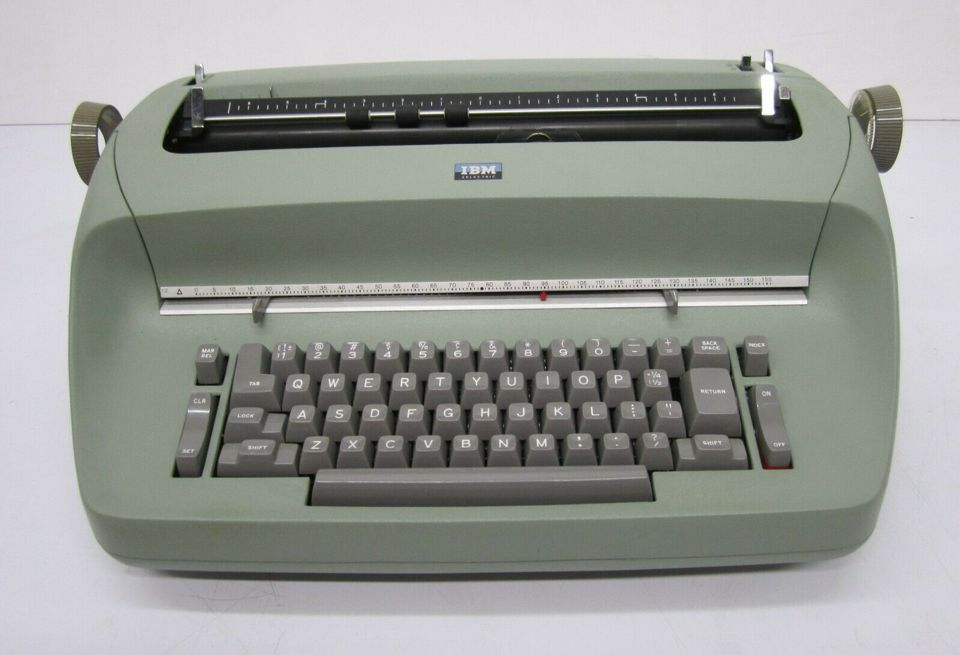
\includegraphics[width=0.46\textwidth]{./Imagenes/Bitmap/selectric.jpg}
     }
     \hfill
     \subfloat[Teclado Bluetooth\label{teclado2}]{%
       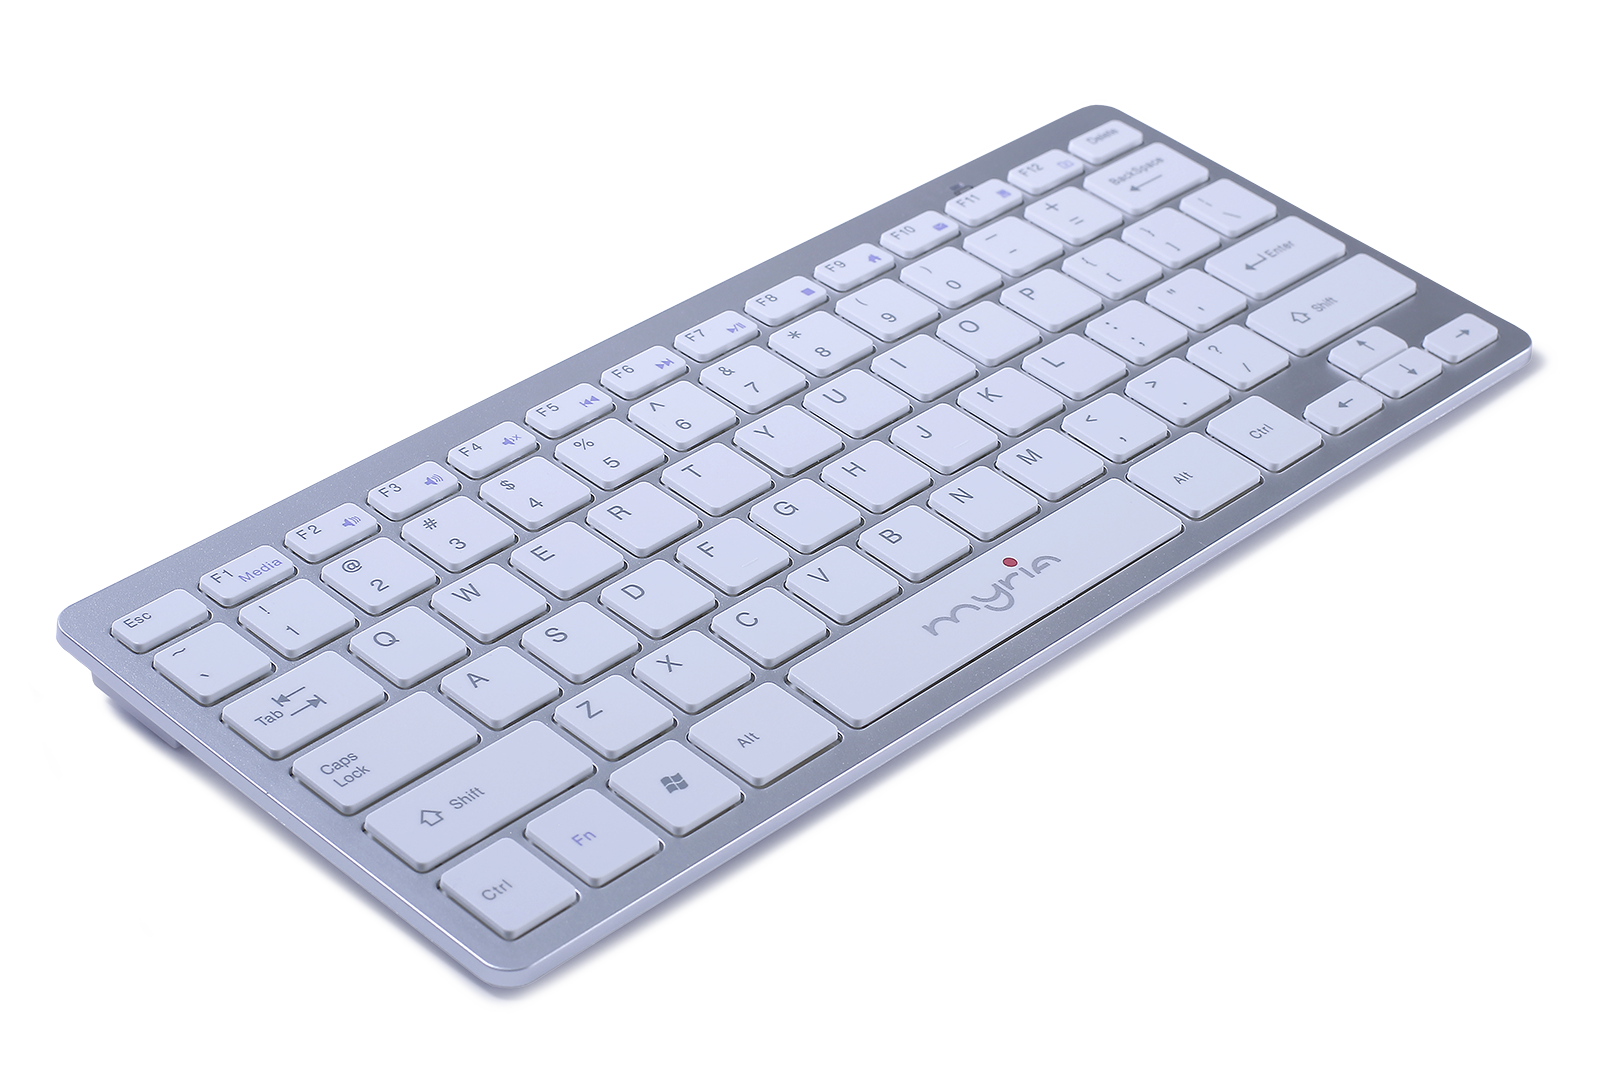
\includegraphics[width=0.46\textwidth]{./Imagenes/Bitmap/tecladoinalambrico.png}
     }
     \caption{Evoluci\'on de los teclados}
     \label{fig:primera}
   \end{figure}
La historia de los teclados actuales tiene su origen en las m\'aquinas de escribir. Estas primeras m\'aquinas de escribir tienen su origen en el a\~no 1877, cuando la empresa Remington las comenz\'o a comercializar de manera masiva. En un primer momento las teclas de dispusieron en orden alfab\'etico, algo que cambiar\'ia un a\~no despu\'es con la aparici\'on de la primera patente del teclado QWERTY (figura~\ref{teclado1}).\footnote{Im\'agen extraida de \url{https://www.fdi.ucm.es/migs/catalogo/selectric/}} Tal y como se\~nala \cite{jimmy}, esta primera versi\'on de las m\'aquinas de escribir ten\'ian un defecto que fue notorio cuando los usuarios escrib\'ian r\'apidamente una sucesi\'on de letras que se encontraban cerca en el teclado. Este defecto consist\'ia en que las barras que conectaban cada una de las teclas chocaban si se pulsaban teclas que estuvieran demasiado cerca.  Para evitar este fallo en el modelo inicial se desarroll\'o el sistema QWERTY, el cual distancia los pares de letras que se suelen escribir juntas.\\

Uno de los primeros avances de estas m\'aquinas de escribir ocurri\'o en la d\'ecada de 1930, cuando se combinaron la tecnolog\'ia de la entrada e impresi\'on de las m\'aquinas de escribir con la tecnolog\'ia de la comunicaci\'on del tel\'egrafo. Este dispositivo fue muy popular durante el siglo XX y sus funciones eran las de enviar y recibir mensajes mecanografiados de un punto a otro a trav\'es de un canal de comunicaci\'on. M\'as adelante fue utilizado en conjunto con las cintas perforadas para almacenar datos en los primeros ordenadores. As\'i, en 1955, el Whirlwind del MIT, se convierte en el primer ordenador del mundo que permite a sus usuarios introducir comandos a trav\'es de un teclado. Adem\'as, confirm\'o lo \'util y conveniente que puede ser un dispositivo de entrada como el teclado.\\

Actualmente las principales mejoras que han sufrido los teclados de ordenador se basan en la eliminaci\'on de cables gracias al Bluetooth (figura~\ref{teclado2})\footnote{Im'agen extraida de \url{https://rb.gy/nia1js}}, la disminuci\'on de la presi\'on que hay que ejercer sobre la tecla para que esta sea detectada y la ergonom\'ia. Con la llegada de los dispositivos t\'actiles se a\~nadi\'o adem\'as el concepto de teclado virtual. Este teclado virtual elimina el uso de un teclado hardware para pasar a un teclado software que imita el teclado tradicional QWERTY pero en una pantalla t\'actil. \\




%%%%%%%%%%%%%%%%%%%%%%%%%%%%%%%%%%%%%%%%%%%%%%%%%%%%%%%%%%%%%%%%%%
\subsection{Evoluci\'on de los ratones}

Adem\'as del teclado, el segundo dispositivo de entrada por excelencia es el rat\'on. La primera maqueta (figura~\ref{Fig:primerraton})\footnote{Im'agen extraida de \url{https://rb.gy/zcyg3x}} fue dise\~nada durante los a\~nos 60, dispon\'ia de 2 ruedas met\'alicas que al desplazarse por una superficie mov\'ian 2 ejes. Cada uno de estos ejes controlaba el movimiento tanto vertical como horizontal del cursor en la pantalla y dispon\'ia de un bot\'on en la parte superior con el que se permit\'ia hacer clic en la posici\'on en la que se encontraba el cursor.\\

\begin{figure}[t]
     \subfloat[Primer rat\'on desarrollado por Douglas Engelbart y Bill English\label{Fig:primerraton}]{%
       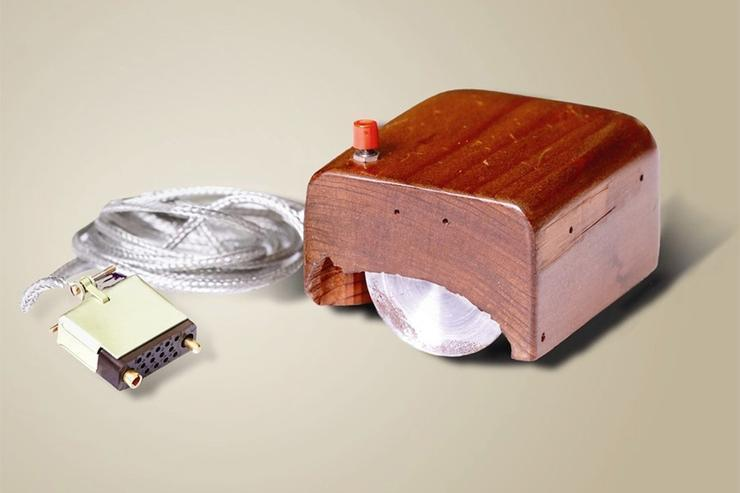
\includegraphics[width=0.5\textwidth]{./Imagenes/Bitmap/Primer_raton.jpg}
     }
     \hfill
\subfloat[Rat\'on del Xerox Alto de los a\~nos 70\label{Fig:xerox}]{%
       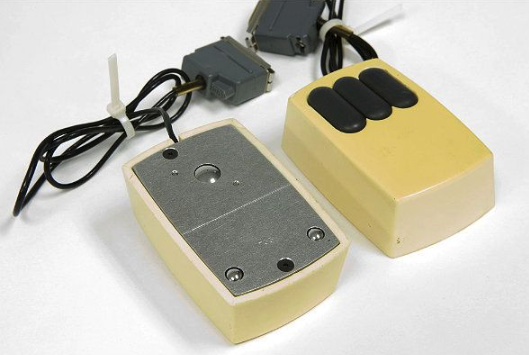
\includegraphics[width=0.5\textwidth]{./Imagenes/Bitmap/xeroxmouse.png}
}
     \caption{Evoluci\'on de los ratones}
     \label{fig:primera}
   \end{figure}


El siguiente avance del dispositivo fue cambiar su carcasa de madera por una de pl\'astico y a\~nadir m\'as botones. Tal y como describi\'o \cite{xerox}, este avance suele ser atribuido a Microsoft o a Apple. Lejos de ser as\'i, fue la empresa \textbf{Xerox} la que realiz\'o el nuevo dise\~no del rat\'on (figura~\ref{Fig:xerox})\footnote{Im'agen extraida de \url{https://rb.gy/dkdej9}} y del que es considerado el primer ordenador personal de la historia junto al Altair 8080. Este nuevo dispositivo sustitu\'ia las 2 ruedas que marcaban la posici\'on del cursor por una \'unica bola de metal. El movimiento de esta bola era la que determinaba la posici\'on del cursor en la pantalla. \\

En el a\~no 1992 Microsoft decidi\'o vender en un mismo paquete su \'ultima versi\'on de MS-DOS y Windows 3.1, lo que hizo que el rat\'on pasase a ser un perif\'erico fundamental. Se dejaba atr\'as el mundo del texto y se abr\'ian a todos los p\'ublicos las interfaces gr\'aficas del PC. Este cambio hizo que el rat\'on siguiera evolucionando y durante la d\'ecada de los 90 e inicios del 2000 los ratones sufrieron algunas mejoras. Algunas de estas mejoras son: una rueda central o lateral para el desplazamiento, el sensor de movimiento \'optico por diodo LED o un sensor basado en un l\'aser no visible. Un sector que aprovech\'o mucho esta estandarizaci\'on del rat\'on y de las interfaces gr\'aficas fue el de los videojuegos. El rat\'on se ha convertido en una parte esencial del mundo de los videojuegos de PC, sirviendo no solo para seleccionar y accionar objetos en pantalla en juegos de estrategia, sino para controlar la c\'amara o cambiar la direcci\'on del personaje en juegos de primera y tercera persona.\\


%%%%%%%%%%%%%%%%%%%%%%%%%%%%%%%%%%%%%%%%%%%%%%%%%%%%%%%%%%%%%%%%%%
\section{Evoluci\'on de los gamepads a trav\'es de las generaciones de consolas}

\begin{figure}[t]
\centering
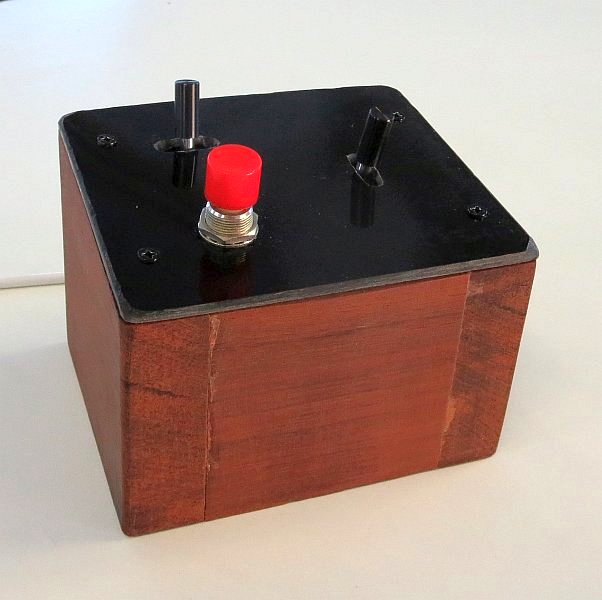
\includegraphics[width=0.4\textwidth]{./Imagenes/Bitmap/spacewar-controller.jpg}
\caption{Joystick utilizado para jugar a Spacewar!}
\label{Fig:spacewar}
\end{figure}
Se dice que el primer intento de videojuego es una patente de 1947 sobre la simulaci\'on del lanzamiento de misiles pero no fue hasta 1958 y el lanzamiento del famoso \textbf{Tenis para Dos} creado por William Higginbotham que se puede comenzar a hablar de videojuegos \citep{tenispara2}. En este juego se recreaba una pista de tenis en la que la pelota iba de un lado a otro de la pista. Poco despu\'es, en 1962 vio la luz \textbf{Spacewar!}. Este t\'itulo fue desarrollado por Steve Russell y posteriormente modificado por sus estudiantes. En este juego lo que se quer\'ia era simular una pelea entre 2 naves en el espacio, fue el primer paso de los juegos multijugador en un mismo dispositivo. El dispositivo de entrada de este juego consist\'ia en 2 ejes de rotaci\'on que se usaban para controlar la rotaci\'on y el empuje de la nave. Adem\'as de esto, el mando dispon\'ia de un bot\'on para disparar misiles (figura~\ref{Fig:spacewar}).\footnote{Im\'agen extraida de \url{https://rb.gy/iaij8s}}\\




Ser\'a en la d\'ecada de los 70 cuando las m\'aquinas recreativas comiencen a tener repercusi\'on con la salida de \textbf{Pong} en 1972 y \textbf{Space Invaders} en 1978. Muchos t\'itulos y sagas tienen su inicio en esta \'epoca en la que las salas de recreativas estaban abarrotadas de j\'ovenes dispuestos a pasar all\'i todas las horas posibles jugando y compitiendo con otros jugadores. Con la salida de las consolas en los a\~nos y d\'ecadas posteriores, las r\'apidas mejoras del hardware y el avance la tecnolog\'ia hizo que las m\'aquinas recreativas se quedasen obsoletas en poco tiempo. Adem\'as de esto la proliferaci\'on de los cibercaf\'es y los juegos en l\'inea hicieron que el consumo de m\'aquinas arcade se estancara. \\

%%%%%%%%%%%%%%%%%%%%%%%%%%%%%%%%%%%%%%%%%%%%%%%%%%%%%%%%%%%%%%%%%%
\subsection{Primera generaci\'on (1972-1976)}

\begin{figure}[t]
     \subfloat[Magnavox Odyssey joystick\label{primera1}]{%
       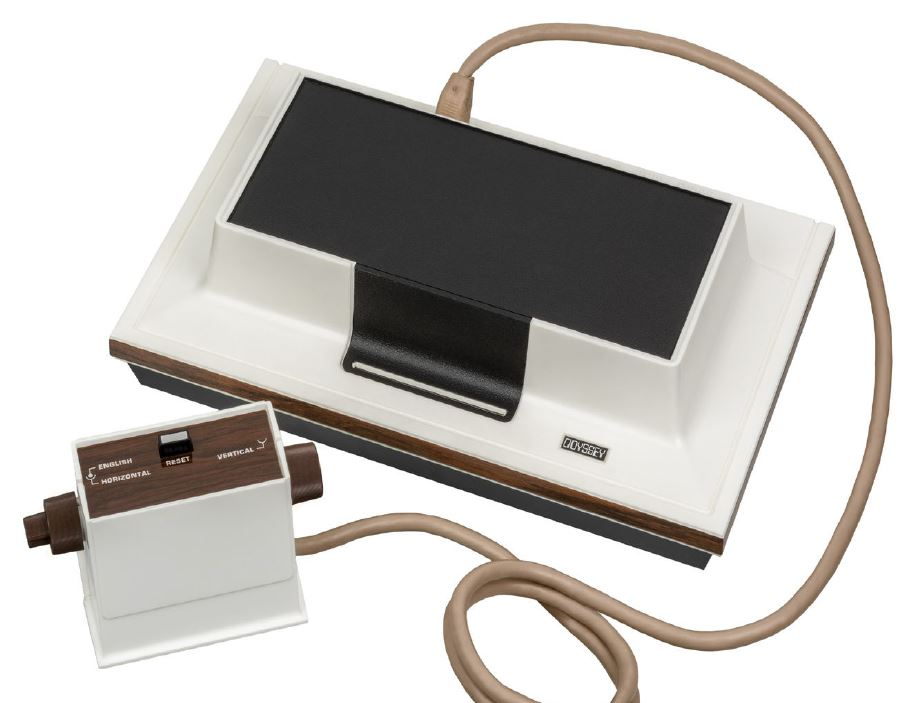
\includegraphics[width=0.4\textwidth]{./Imagenes/Bitmap/Magnavox-Odyssey-Controller.jpg}
     }
     \hfill
     \subfloat[Rifle de luz Magnavox Odyssey Shooting Gallery\label{primera2}]{%
       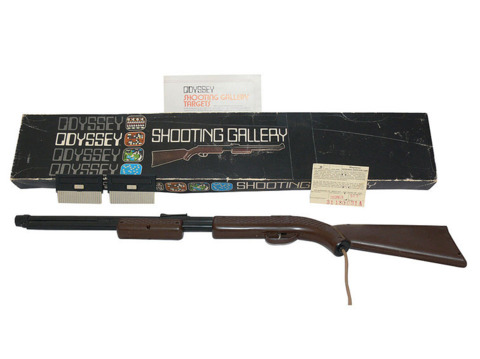
\includegraphics[width=0.4\textwidth]{./Imagenes/Bitmap/pistolaluz.jpg}
     }
     \caption{Dispositivos de entrada relevantes en la 1"a  generaci\'on de consolas}
     \label{fig:primera}
   \end{figure}

En 1972 fue lanzada de manera oficial la \textbf{Magnavox Odyssey}, considerada la primera videoconsola. El dispositivo de entrada para poder jugar consist\'ia de 2 diales que se utilizaban para el movimiento horizontal y vertical del personaje como puede verse en la figura~\ref{primera1}. Durante ese mismo a\~no, la misma Magnavox sac\'o su juego de disparos conocido como \textit{Magnavox Odyssey Shooting Gallery}. Este juego ten\'ia la particularidad de que ten\'ia que ser jugado con un mando diferente al original de la consola. Este accesorio nuevo era una pistola de luz (figura~\ref{primera2}).\footnote{Im\'agen extraida de \url{https://rb.gy/5tfxml}} El funcionamiento de este nuevo mando era que los disparos se registraban siempre y cuando la pistola apuntase a una luz intensa por lo que si el jugador apuntaba hacia una bombilla, el juego marcaba como ``alcanzado'' el primer objetivo de la pantalla. La primera soluci\'on de este problema fue dibujar la pantalla en negro una vez el objetivo es alcanzado para as\'i comprobar que se est\'a apuntando a la pantalla, esto se desarrolar\'ia en posteriores juegos. \\




%%%%%%%%%%%%%%%%%%%%%%%%%%%%%%%%%%%%%%%%%%%%%%%%%%%%%%%%%%%%%%%%%%
\subsection{Segunda generaci\'on (1976-1983)}


En 1976 la empresa Fairchild Semiconductor sac\'o al mercado la \textbf{Fairchild Channel F} cuya caracter\'istica principal a nivel de entrada de usuario fue la incorporaci\'on de un joystick de 8 direcciones.  Adem\'as, la parte de arriba de este mando pod\'ia girarse para ser compatible con juegos como \textit{Pong} y tambi\'en pod\'ia ser pulsado y usarse normalmente como bot\'on de disparo, tal y como puede verse en la figura~\ref{segunda1}.\\

En 1977 sali\'o al mercado uno de los joysticks m\'as famosos. Este joystick es el que se utilizaba en la consola \textbf{Atari VCS} que posteriormente ser\'ia conocida como \textbf{Atari 2600}. Este joystick se conoc\'ia como el \textbf{Atari CX40} y consist\'ia de una palanca que permit\'ia un movimiento en 8 direcciones y un bot\'on (figura~\ref{segunda2}). Junto con este modelo, Atari sac\'o al mercado un tipo de conexi\'on que se convertir\'ia en el est\'andar de facto. Los sistemas posteriores eran compatibles con estos joysticks ya que lo tomaron como referencia. Unos pocos a\~nos despu\'es, en 1982, Atari lanz\'o su nueva consola Atari 5200. El sistema combinaba un dise\~no mec\'anico demasiado complejo con un sistema de circuito flexible interno de muy bajo coste. Este controlador incluy\'o un bot\'on de pausa, una caracter\'istica \'unica en ese momento (figura~\ref{segunda3}).\\


\begin{figure}[t]
     \subfloat[Fairchild Channel F joystick\label{segunda1}]{%
       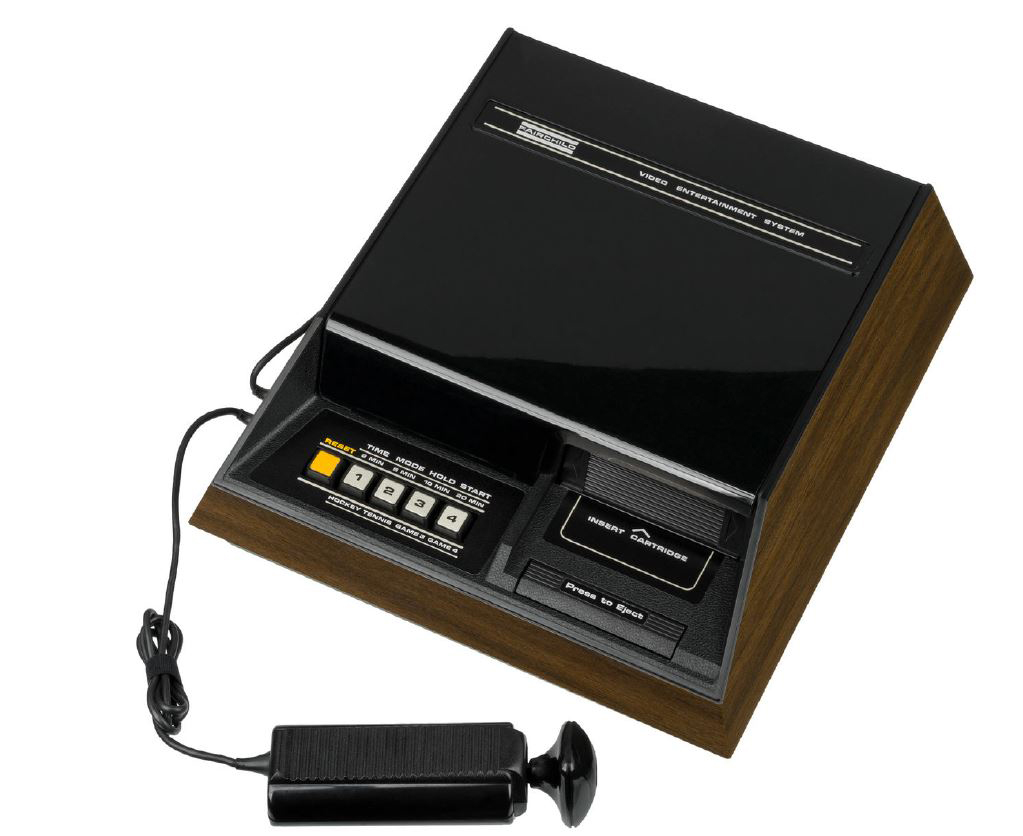
\includegraphics[width=0.3\textwidth]{./Imagenes/Bitmap/Fairchild.jpg}
     }
     \hfill
     \subfloat[AtariCX40\label{segunda2}]{%
       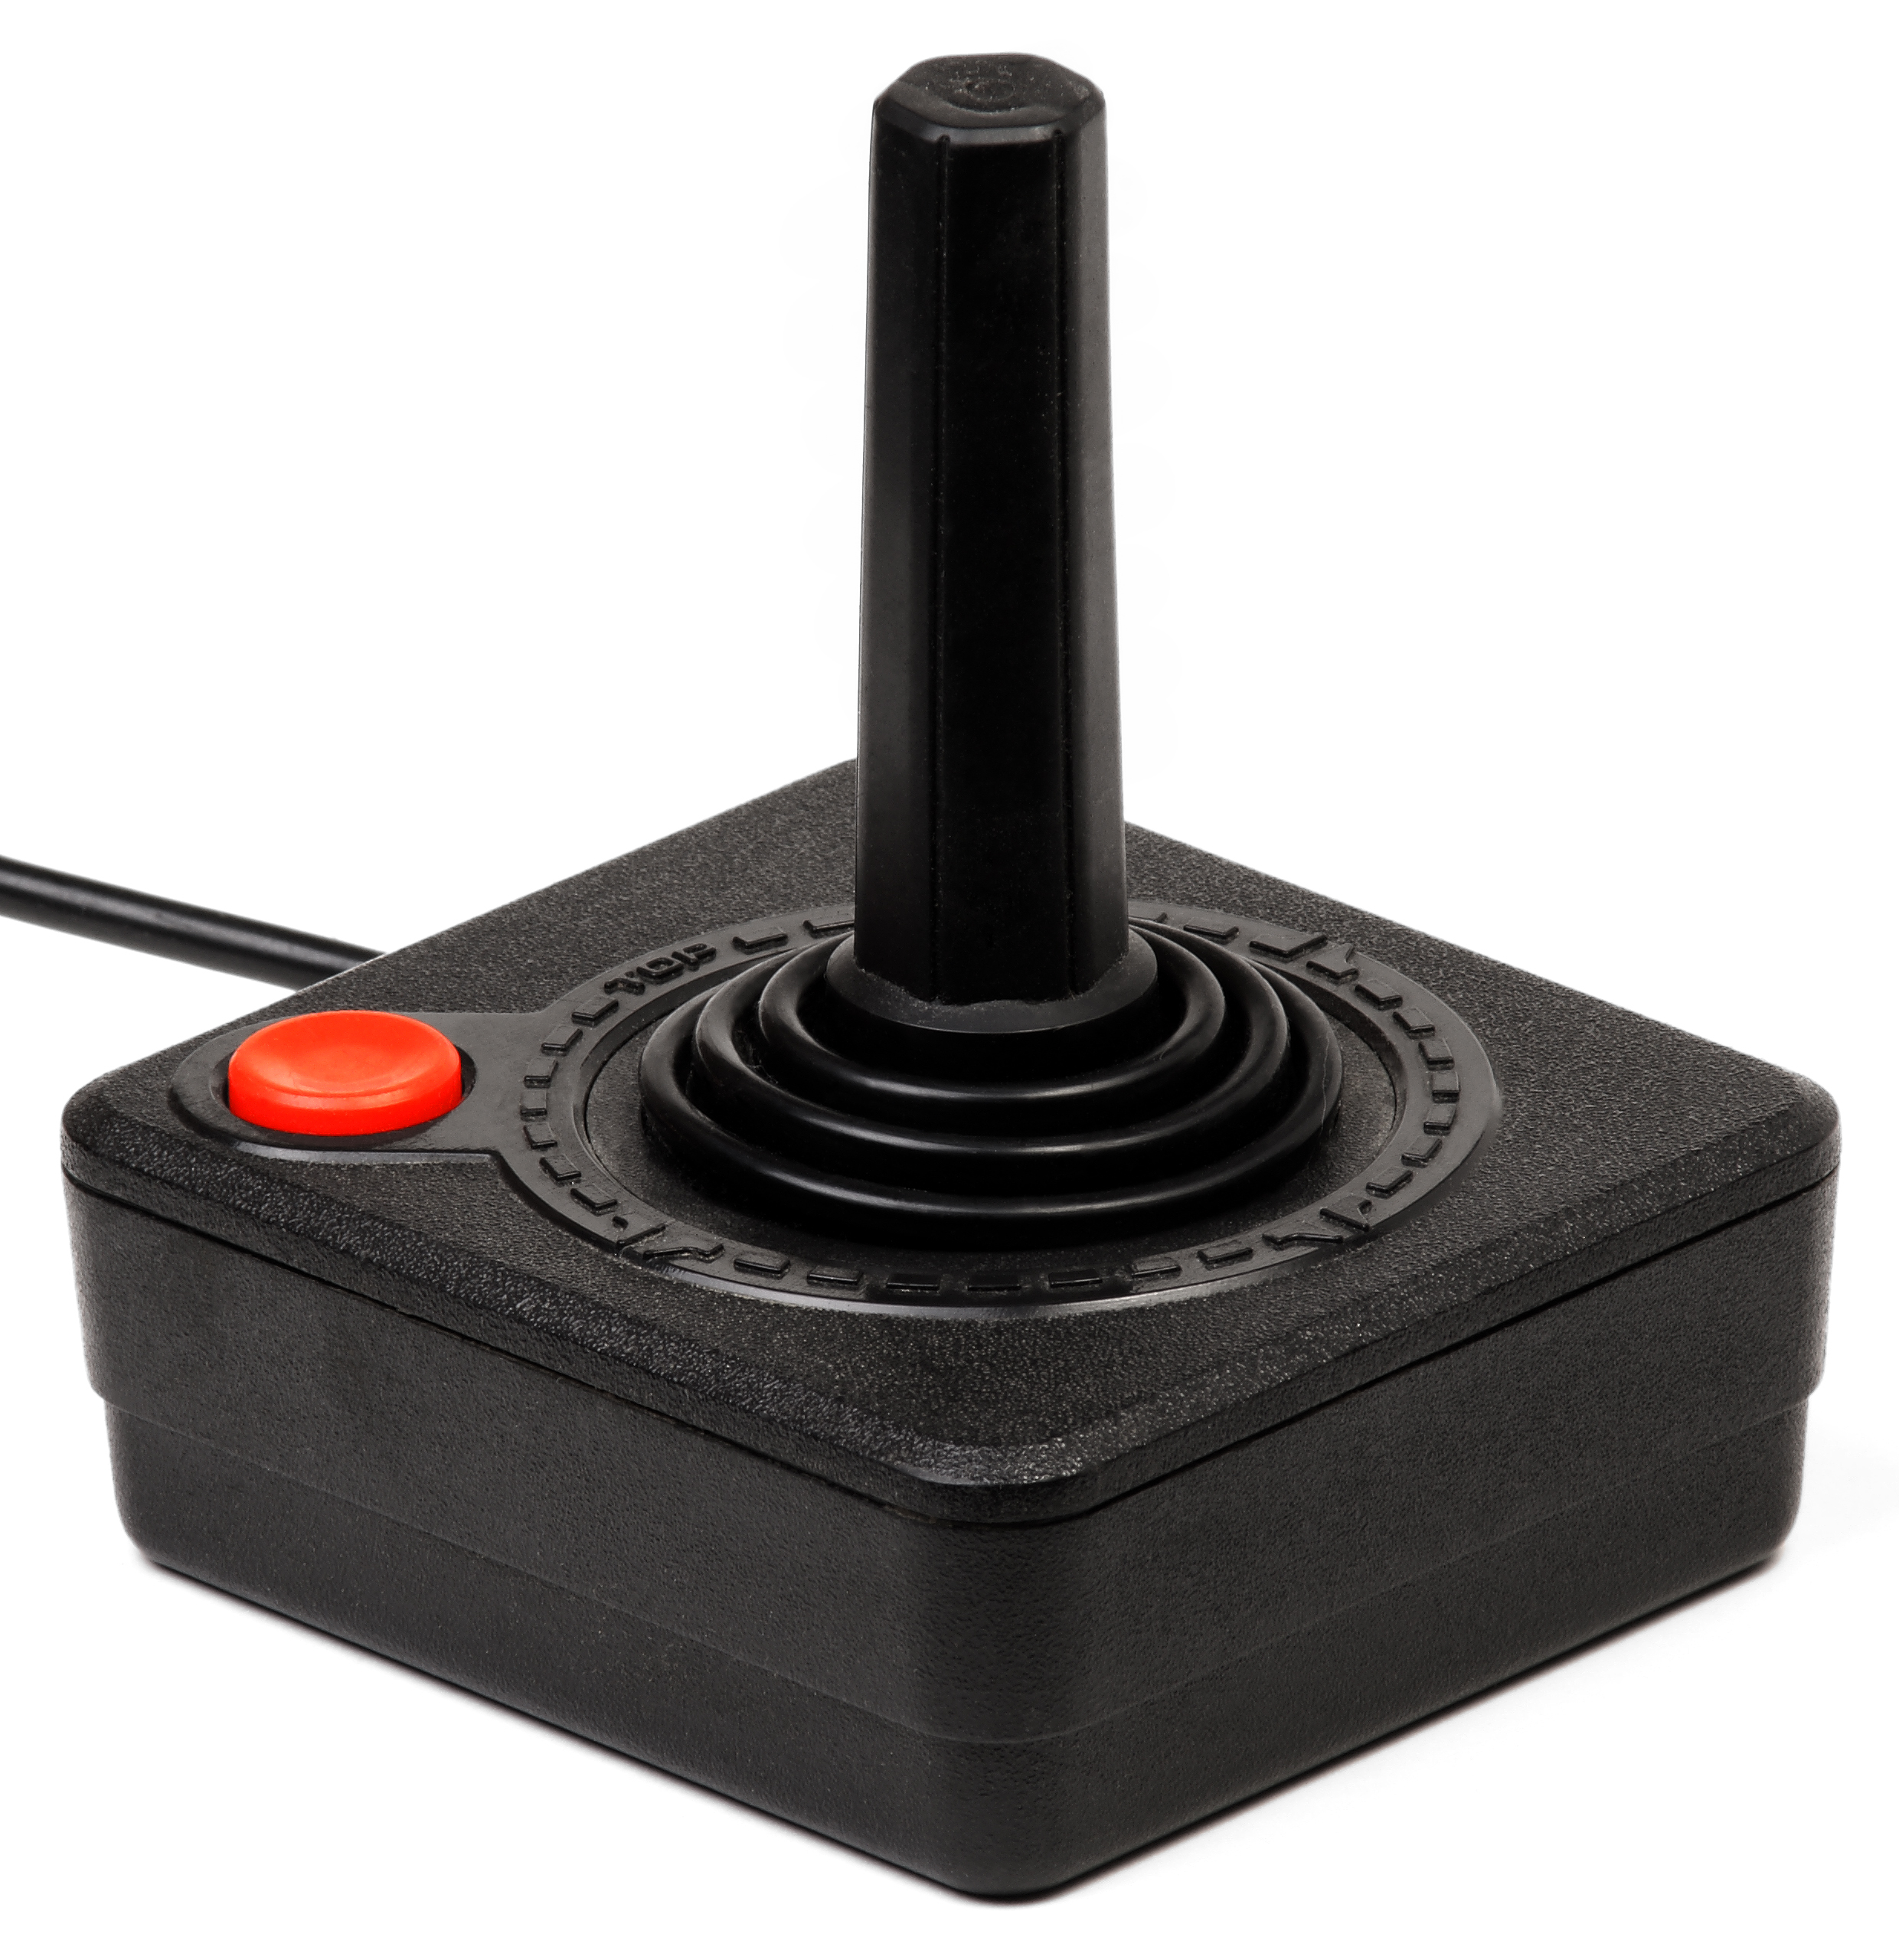
\includegraphics[width=0.3\textwidth]{./Imagenes/Bitmap/Atari-2600-Joystick.jpg}
     }
\hfill
     \subfloat[Atari 5200 joystick\label{segunda3}]{%
       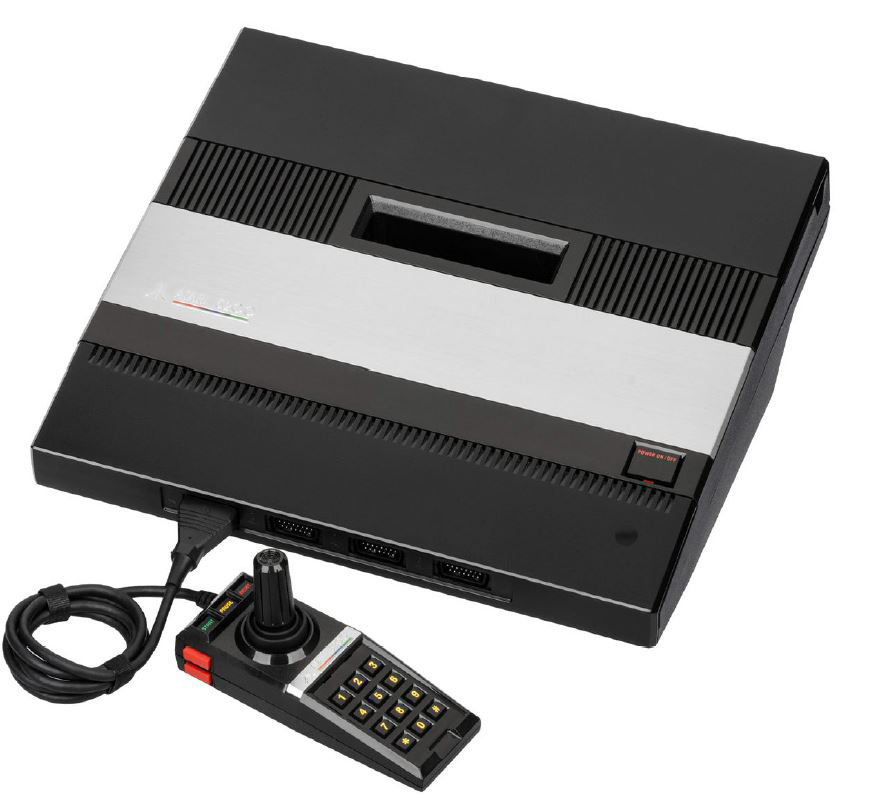
\includegraphics[width=0.3\textwidth]{./Imagenes/Bitmap/1200px-Atari-5200-Controller.jpg}
     }
     \caption{Dispositivos de entrada relevantes en la 2"a  generaci\'on de consolas}
     \label{fig:segunda}
   \end{figure}

%%%%%%%%%%%%%%%%%%%%%%%%%%%%%%%%%%%%%%%%%%%%%%%%%%%%%%%%%%%%%%%%%%
\subsection{Tercera generaci\'on (1983-1987)}


En 1983 Nintendo sac\'o al mercado \textbf{Nintendo Entertainment System (NES)}. El controlador de esta consola no fue el primer dispositivo donde se utiliz\'o pero el \'exito de la consola lo populariz\'o. Esta cruceta permit\'ia un movimiento en 4 direcciones y que pretend\'ia reemplazar a las voluminosas palancas de mando de los controladores. Adem\'as de la cruceta, el mando dispon\'ia de 2 botones redondos (A y B) y otros 2 botones rectangulares (START y SELECT) tal y como puede verse en la figura~\ref{tercera1}. Posteriormente, se lanzaron varios dispositivos especiales dise\~nados precisamente para usarse con juegos espec\'ificos, aunque muy pocos de estos se volvieron populares. Uno de estos dispositivos era el \textbf{Power Glove} (figura~\ref{tercera2}),\footnote{Im'agen extraida de \url{https://rb.gy/jnxtil}} el que ser\'ia considerado como uno de los primeros perif\'ericos de interfaz en recrear los movimientos en tiempo real de la mano en una pantalla de televisi\'on o de un ordenador. \\

En 1985 Sega entr\'o en el mundo de las consolas con el lanzamiento de la \textbf{Sega Master System}, figura~\ref{tercera3}. El controlador de la Master System tiene 2 versiones, una de ellas tiene un una cruceta y otra tiene una palanca para el movimiento. Esta nueva cruceta fue un intento de mejora de la cruceta que usaba Nintendo en la NES. 

\begin{figure}[t]
     \subfloat[Mando NES\label{tercera1}]{%
       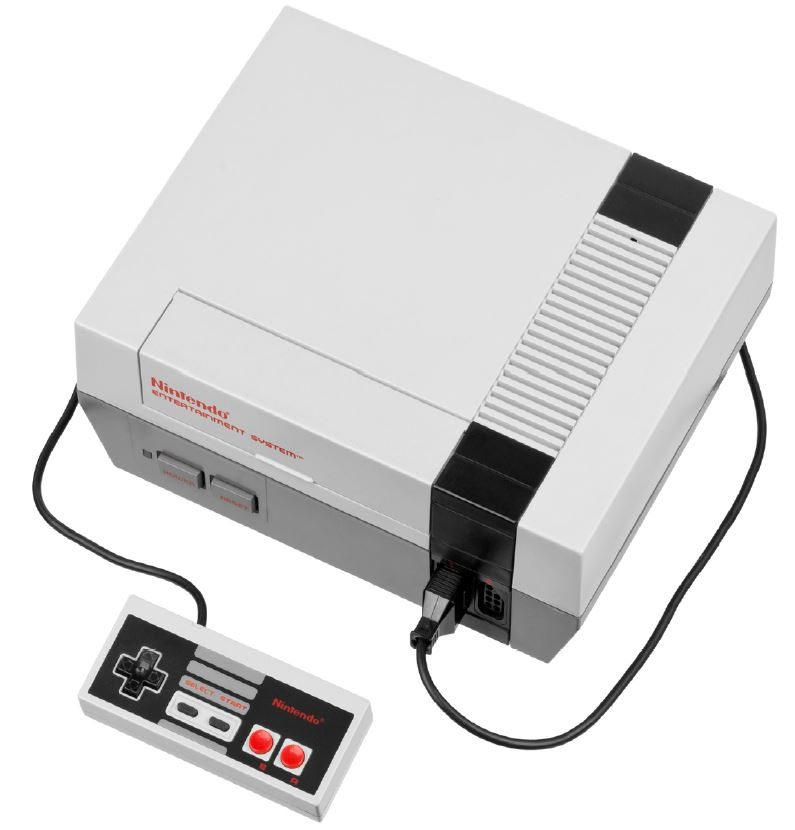
\includegraphics[width=0.3\textwidth]{./Imagenes/Bitmap/NESgamepad.jpg}
     }
     \hfill
     \subfloat[Power Glove NES\label{tercera2}]{%
       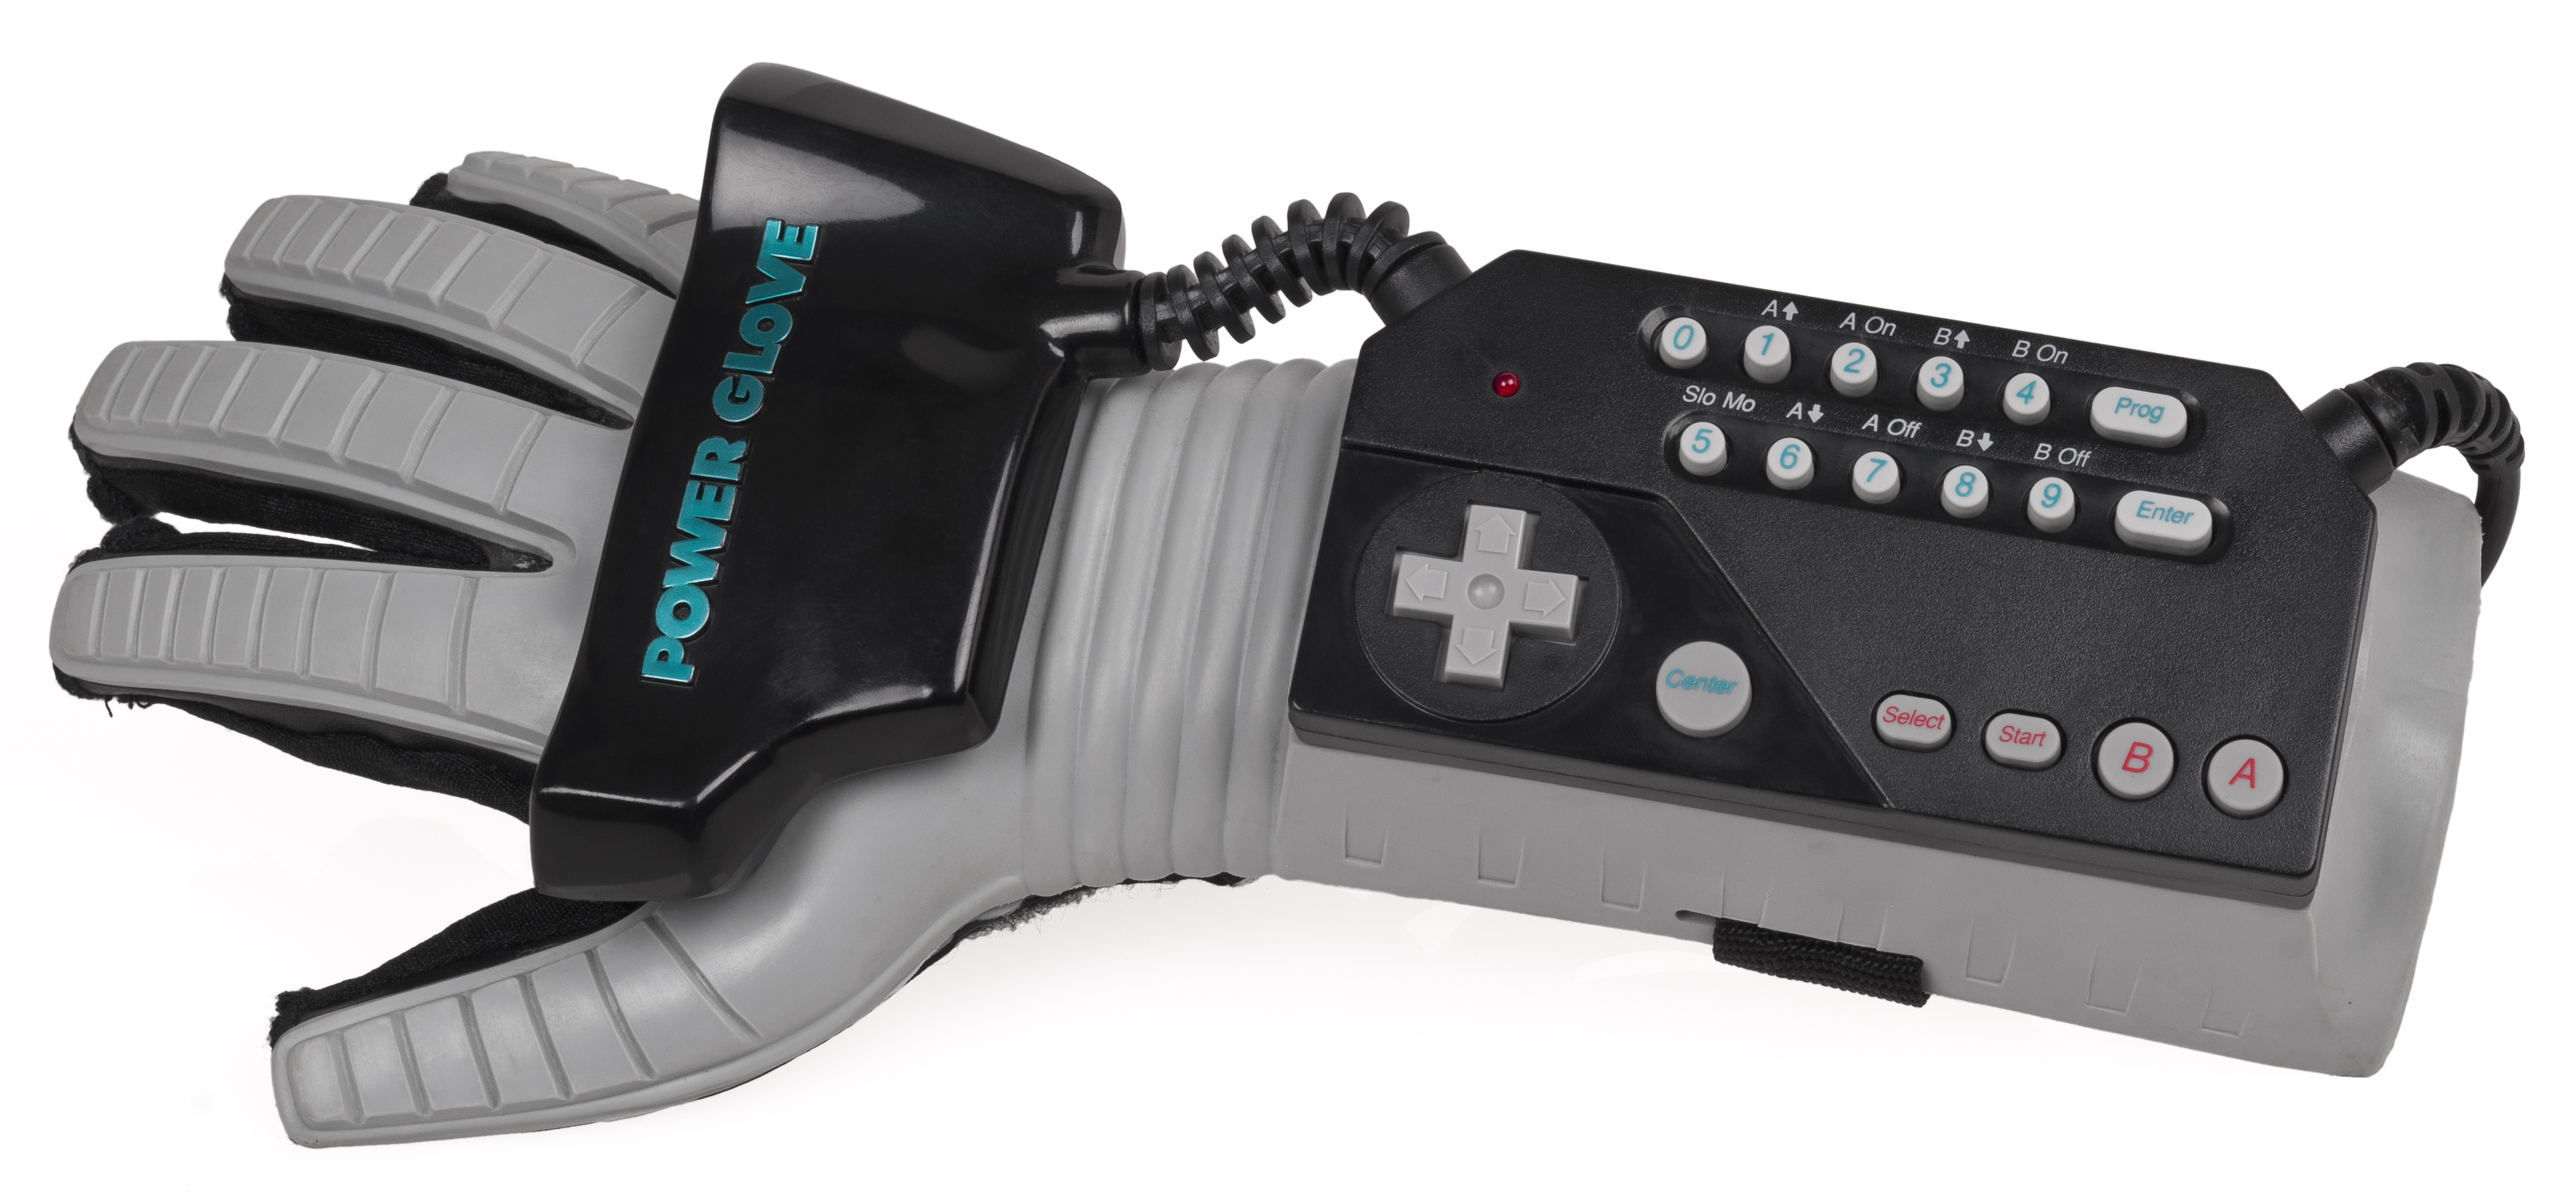
\includegraphics[width=0.3\textwidth]{./Imagenes/Bitmap/NES-Power-Glove.jpg}
     }
 \hfill
     \subfloat[Sega Master System\label{tercera3}]{%
       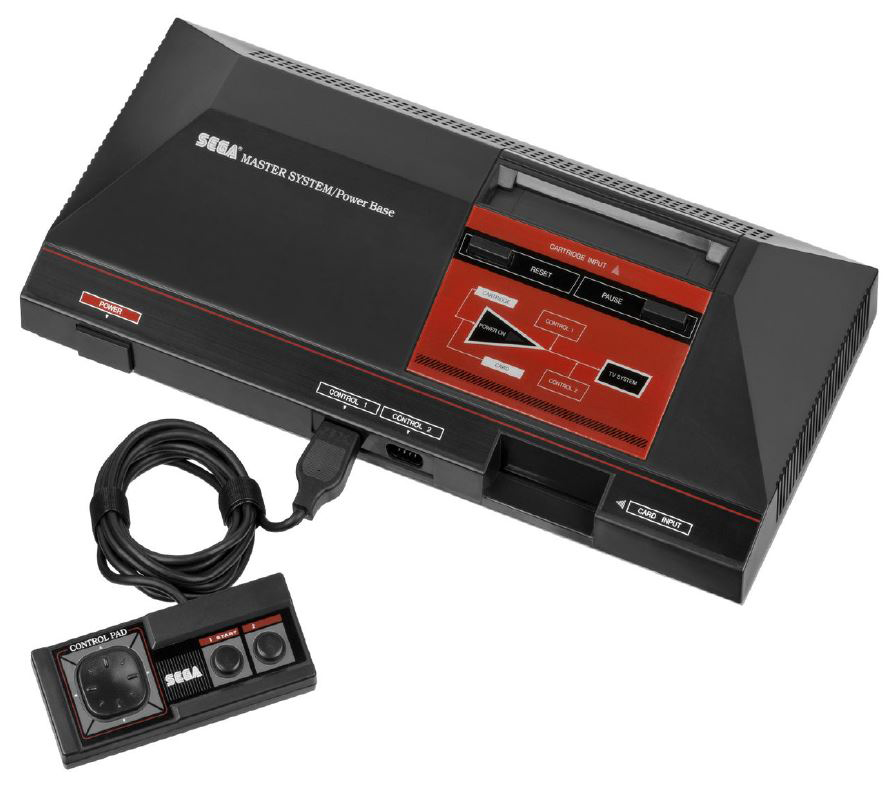
\includegraphics[width=0.3\textwidth]{./Imagenes/Bitmap/Sega Master System.JPG}
     }
     \caption{Dispositivos de entrada relevantes en la 3"a  generaci\'on de consolas}
     \label{fig:tercera}
   \end{figure}

%%%%%%%%%%%%%%%%%%%%%%%%%%%%%%%%%%%%%%%%%%%%%%%%%%%%%%%%%%%%%%%%%%

\subsection{Cuarta generaci\'on (1987-1993)}

En 1988 la compa\~nia Sega lanz\'o al mercado su nueva consola, la \textbf{Sega Mega Drive}, figura~\ref{cuarta3}. El controlador de esta consola abandon\'o el dise\~no cuadrado y pas\'o a darle m\'as importancia a la ergonom\'ia. El controlador dispon\'ia de una cruceta, un bot\'on central de START y 3 botones en su lado derecho. Posteriormente se hicieron versiones del mando que inclu\'ian 6 botones en la parte derecha del mando en lugar de 3.\\


En 1990 Nintendo hizo evolucionar a la Nintendo NES y lanz\'o la \textbf{Super Nintendo Entertainment System (SNES)} (figura~\ref{cuarta2}), la cual dej\'o atr\'as un dise\~no cuadrado del controlador y se inclin\'o por un dise\~no m\'as ergon\'omico, se mejor\'o la cruceta y se a\~nadieron otros 2 botones (X e Y). \\

Dentro de la evoluci\'on de los controladores, en 1993 la compa\~n\'ia SEGA sorprendi\'o con el lanzamiento de un nuevo accesorio para su consola \textbf{Sega Mega Drive}. Este accesorio consist\'ia en un aro octogonal que se colocaba en el suelo y se conectaba directamente al puerto de controlador de la consola. Lo llamaron \textbf{Sega Activator} (figura~\ref{cuarta1})\footnote{Im'agen extraida de \url{https://rb.gy/jzltmg}} y fue el primer controlador en el que se utilizaba el cuerpo completo para jugar. El jugador se ten\'ia que situar en el centro del aro, el cual emit\'ia rayos infrarrojos hacia arriba para detectar los movimientos del jugador. Los juegos destinados al Sega Activator eran juegos que involucraban el movimiento de brazos y piernas para que el jugador cruzase los rayos infrarrojos y as\'i se detectase el movimiento. Al tratarse de 8 segmentos, cada uno de estos segmentos estaba mapeado como si fuera un bot\'on en el mando tradicional, el cual se ``pulsar\'ia'' cada vez que el jugador cruzase un segmento de los rayos infrarrojos. \\


\begin{figure}[t]
\subfloat[Sega Mega Drive\label{cuarta3}]{%
       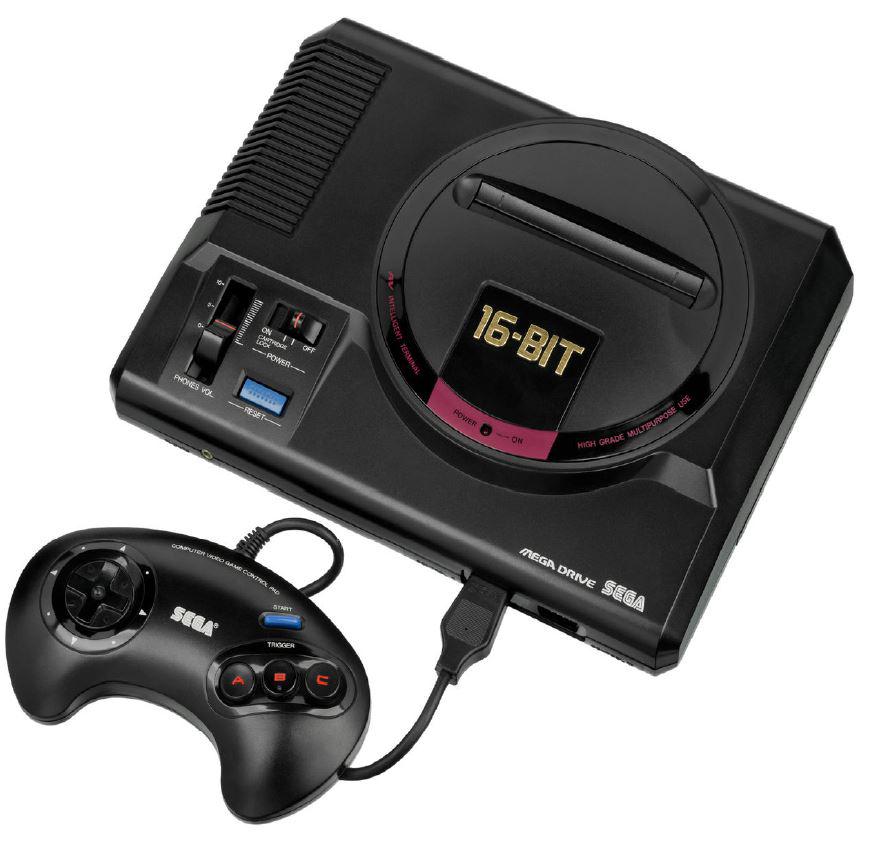
\includegraphics[width=0.3\textwidth]{./Imagenes/Bitmap/MegaDrive.JPG}
     }
     \hfill
\subfloat[Super Nintendo joystick\label{cuarta2}]{%
       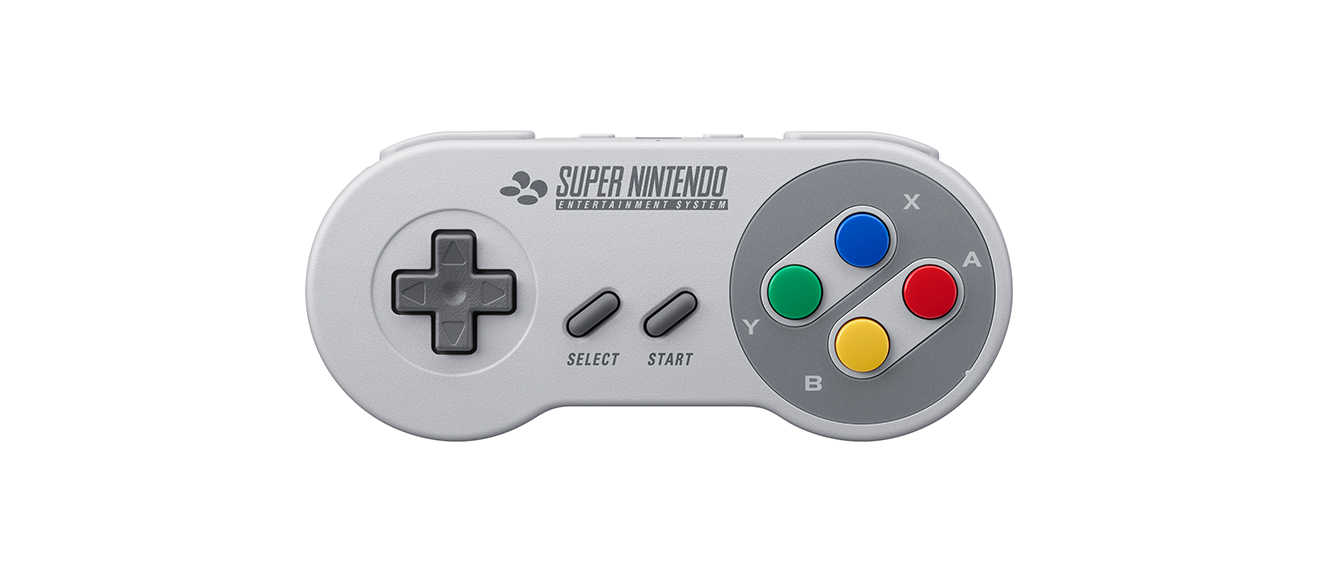
\includegraphics[width=0.3\textwidth]{./Imagenes/Bitmap/SNES.jpg}
     }
     \hfill
     \subfloat[Sega Activator\label{cuarta1}]{%
       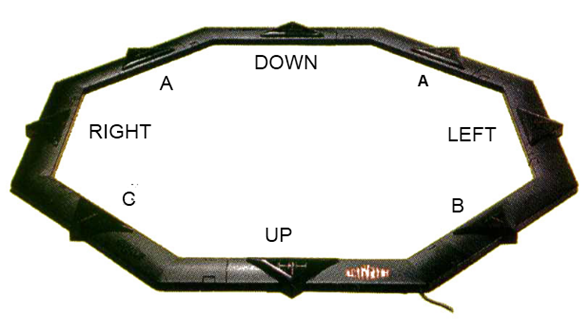
\includegraphics[width=0.3\textwidth]{./Imagenes/Bitmap/SEGAActivator.png}
     }
     \caption{Dispositivos de entrada relevantes en la 4"a  generaci\'on de consolas}
     \label{fig:cuarta}
   \end{figure}
%%%%%%%%%%%%%%%%%%%%%%%%%%%%%%%%%%%%%%%%%%%%%%%%%%%%%%%%%%%%%%%%%%

\subsection{Quinta generaci\'on (1993-1998)}



Durante los a\~nos 90 \textbf{Sony} entr\'o al terreno del desarrollo de consolas y por consecuencia, de modelos diferentes de controladores de videojuegos. Con su primera consola, la \textbf{Sony PlayStation}, incluyeron un nuevo dise\~no de mando que recog\'ia muchos de los dise\~nos vistos hasta el momento. A diferencia de Nintendo, este controlador cambi\'o la nomenclatura de los botones A, B, Y y X por las figuras $\triangle$, $\textbigcircle$, $\times$ y $\Box$, manten\'ia la cruceta y los botones START y SELECT y adem\'as a\~nadi\'o 4 botones m\'as en la parte lateral del mando para los dedos \'indice y coraz\'on. 3 a\~nos m\'as tarde Sony sacar\'ia una re-edici\'on del mando al que le incorporaron 2 sticks anal\'ogicos junto con un bot\'on con un LED para cambiar entre los diferentes modos usados para el control del personaje (figura~\ref{quinta3}). \'Unicamente la versi\'on japonesa presentaba una funci\'on de retroalimentaci\'on de vibraci\'on. \\

Por el lado de Nintendo, la consola sucesora de la Super Nintendo fue la \textbf{Nintendo 64} que fue acompa\~nada por un nuevo dise\~no de mando que no pas\'o desapercibido (figura~\ref{quinta1}). Dispon\'ia de una cruceta en la parte izquierda del mando, un stick de 360 grados y un bot\'on START en el centro del mando y 6 botones en su parte derecha. Complementario a esto, en la parte trasera del mando hab\'ia 2 botones m\'as y tambi\'en en la parte trasera se daba la opci\'on de introducir un dispositivo extra\'ible que proporcionaba retroalimentaci\'on de vibraci\'on (figura~\ref{quinta2}).\footnote{Im'agen extraida de \url{https://rb.gy/9totoz}} Este accesorio se activaba en ocasiones concretas como al disparar un arma y serv\'ia para sumergir al jugador en el videojuego.\\

\begin{figure}[t]
 \subfloat[Dualshock con sticks anal\'ogicos\label{quinta3}]{%
       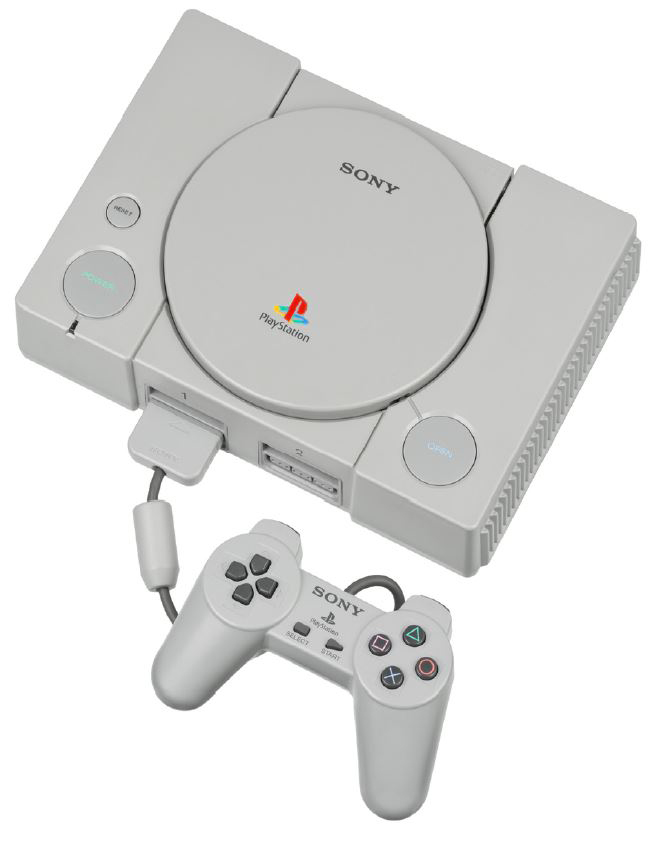
\includegraphics[width=0.3\textwidth]{./Imagenes/Bitmap/Dualshock.jpg}
     }
\hfill
     \subfloat[Mando Nintendo 64\label{quinta1}]{%
       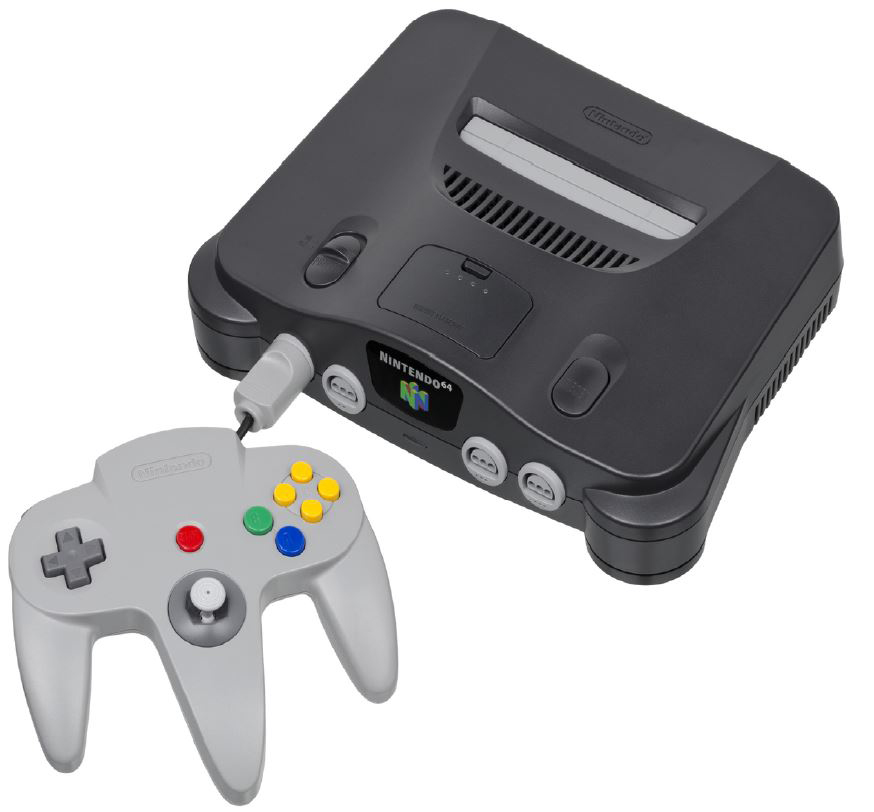
\includegraphics[width=0.3\textwidth]{./Imagenes/Bitmap/N64-Console-Set.jpg}
     }
     \hfill
 \subfloat[Rumble Pack Nintendo 64\label{quinta2}]{%
       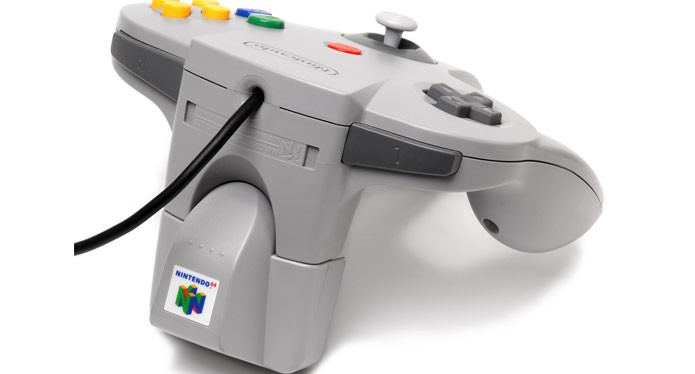
\includegraphics[width=0.3\textwidth]{./Imagenes/Bitmap/rumble-pack-64.jpg}
     }
     \caption{Dispositivos de entrada relevantes en la 5"a  generaci\'on de consolas}
     \label{fig:quinta}
   \end{figure}

%%%%%%%%%%%%%%%%%%%%%%%%%%%%%%%%%%%%%%%%%%%%%%%%%%%%%%%%%%%%%%%%%%

\subsection{Sexta generaci\'on (1998-2005)}

En los a\~nos posteriores las compa\~n\'ias siguieron sacando diferentes mandos que modificaban tama\~no y posiciones de los botones pero no salieron cambios significativos hasta que en 2002 Nintendo lanz\'o al mercado un nuevo mando alternativo para su consola \textbf{GameCube}, este controlador ten\'ia la peculiaridad de ser inal\'ambrico. Lo llamaron \textbf{WaveBird Wireless Controller} (figura~\ref{sexta1})\footnote{Im'agen extraida de \url{https://rb.gy/wns7qv}} y sent\'o las bases para los pr\'oximos mandos inal\'ambricos. Contaba con una cruceta, 6 botones digitales, 2 botones h\'ibridos ya que hac\'ian la funci\'on de gatillos y 2 palancas anal\'ogicas para el movimiento del personaje y la c\'amara normalmente. Como alimentaci\'on usaba 2 pilas AA y para comunicarse con la consola usaba radiofrecuencia, lo que permit\'ia al jugador alejarse hasta 6 metros de la consola. Poco tiempo despu\'es tanto Sony con su PlayStation 3 como Microsoft con su Xbox 360 a\~nadir\'ian las bater\'ias a sus mandos para convertirlos en inal\'ambricos. \\

En el a\~no 2001 Microsoft lanz\'o al mercado su primera consola que adem\'as fue fruto de una colaboraci\'on con Intel. Su principal caracter\'istica es su procesador central basado en el procesador Pentium III de Intel, adem\'as incorporaba un lector de DVD, un puerto ethernet y la posibilidad de conectar 4 mandos.

\begin{figure}[t]
     \subfloat[WaveBird Wireless Controller\label{sexta1}]{%
       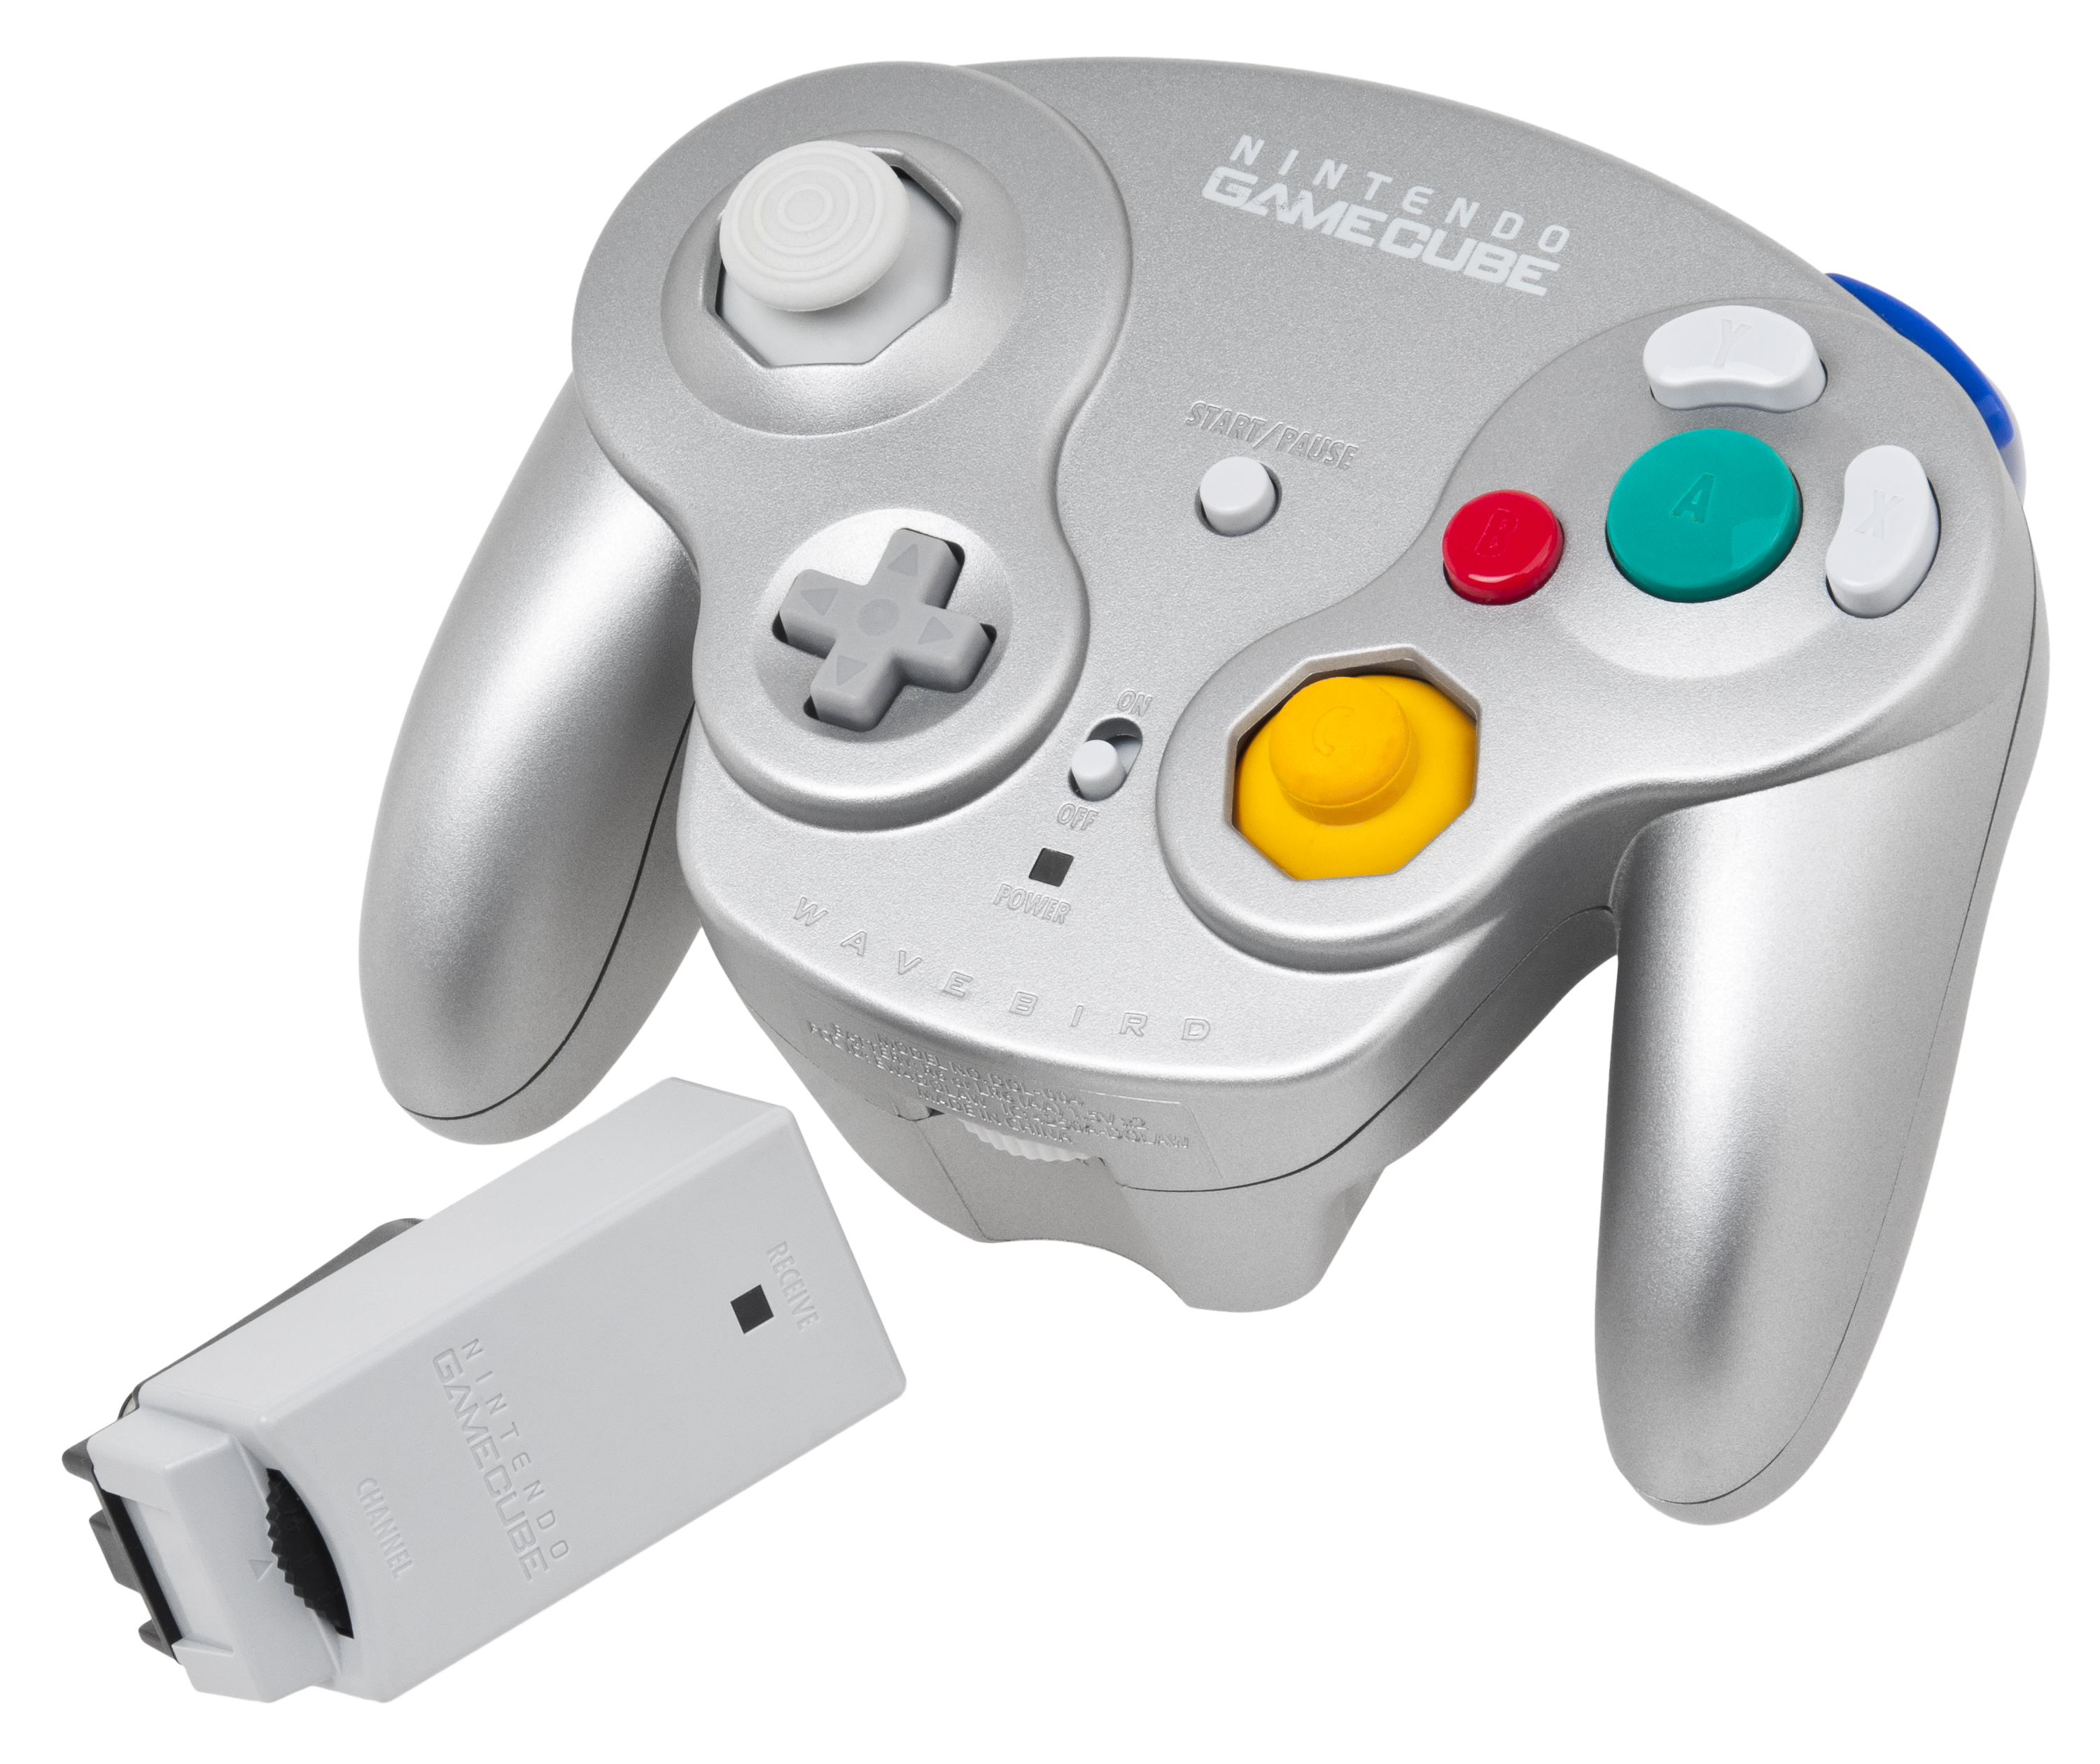
\includegraphics[width=0.4\textwidth]{./Imagenes/Bitmap/Nintendo-GameCube-Wavebird-Silver.jpg}
     }
     \hfill
\subfloat[Joystick original GameCube\label{sexta2}]{%
       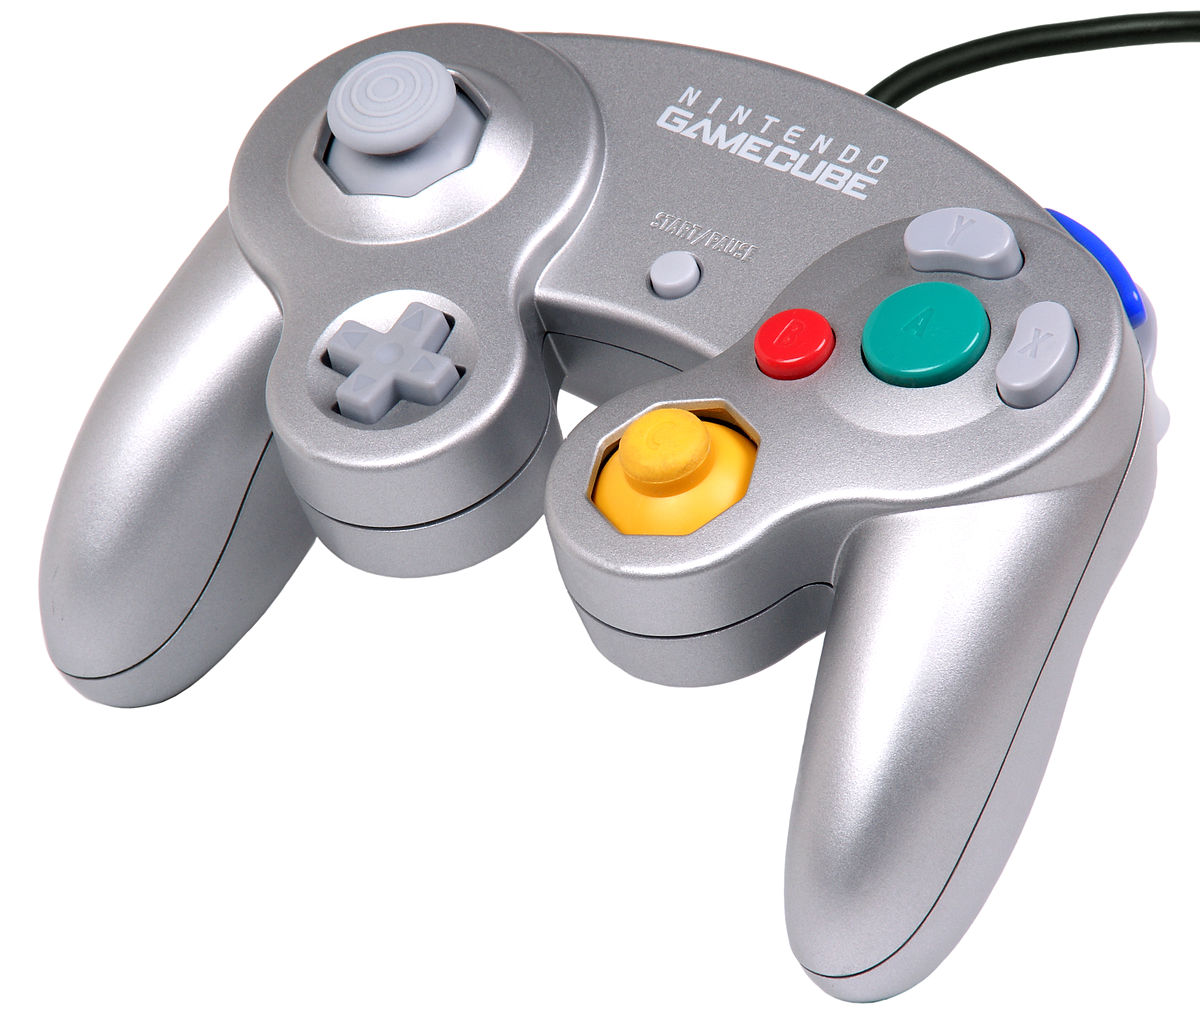
\includegraphics[width=0.4\textwidth]{./Imagenes/Bitmap/1200px-Gamecube-controller.jpg}
     }
     \caption{Dispositivos de entrada relevantes en la 6"a  generaci\'on de consolas}
     \label{fig:sexta}
   \end{figure}

%%%%%%%%%%%%%%%%%%%%%%%%%%%%%%%%%%%%%%%%%%%%%%%%%%%%%%%%%%%%%%%%%%

\subsection{S\'eptima generaci\'on (2005-2012)}

\begin{figure}[t]
     \subfloat[Barra de sensores infrarrojos Wii\label{septa1}]{%
       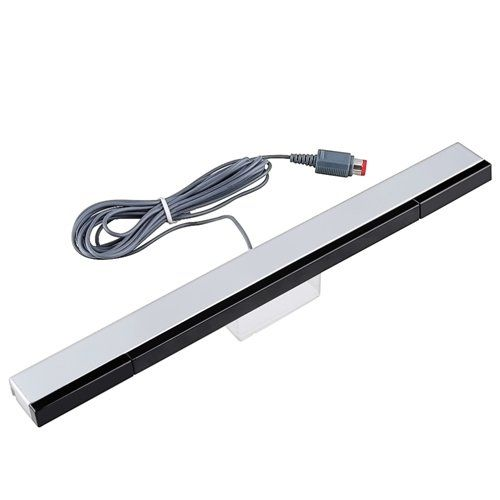
\includegraphics[width=0.5\textwidth]{./Imagenes/Bitmap/barra-sensor-infrarrojos-para-nintendo-wii-con-cable_3.jpg}
     }
     \hfill
\subfloat[Wiimote y Nunchuck\label{septa2}]{%
       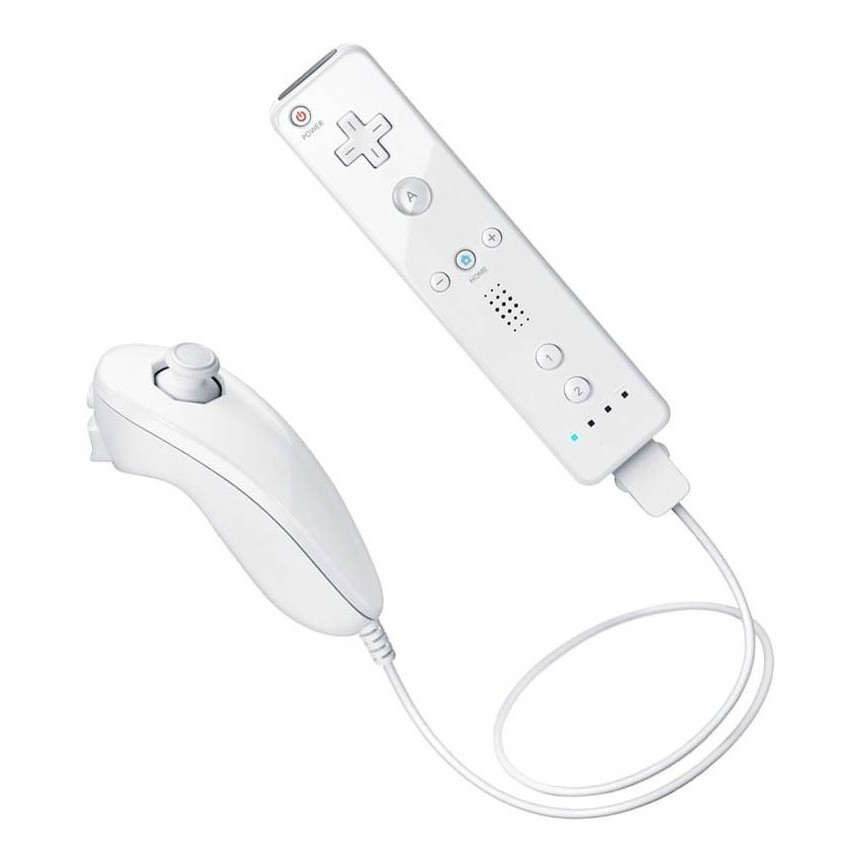
\includegraphics[width=0.5\textwidth]{./Imagenes/Bitmap/wiimote_nunchuck.jpg}
     }
     \caption{Dispositivos de entrada relevantes de Nintendo en la 7"a  generaci\'on}
     \label{fig:septima}
   \end{figure}

En 2006 Nintendo lanz\'o al mercado una consola cuyo objetivo principal era ser usada por todos los miembros de la casa. Esta consola fue \textbf{Wii} y trajo consigo la caracter\'istica m\'as importante de esta consola, una nueva versi\'on de mando. El \textbf{Wiimote} o \textbf{Wii Remote} tiene la capacidad de detectar movimiento en los 3 ejes mediante el uso de aceler\'ometros y la de apuntar. A diferencia de lo que ocurr\'ia con las pistolas de luz, la detecci\'on de la direcci\'on del apuntado ven\'ia dado por una barra de sensores con LED infrarrojos (figura~\ref{septa1}).\footnote{Im'agen extraida de \url{https://rb.gy/kemiaw}} Para lograr detectar la direcci\'on a la que el Wiimote apunta, el dispositivo incorpora en su parte superior un sensor \'optico \textit{PixArt}. Este dispositivo incluido en una barra de 10 sensores LED infrarrojos, permit\'ian al jugador apuntar de manera precisa hasta 5 metros de distancia de la barra. Para que el apuntado fuese m\'as preciso la barra deb\'ia colocarse encima o debajo de la televisi\'on.\\

El dise\~no del controlador es similar a los control remoto de televisi\'on para as\'i hacer que sea lo m\'as intuitivo posible. En su parte frontal, el Wiimote dispone de los botones A, 1, 2, +, -, HOME, POWER y una cruceta. Adem\'as de estos botones el mando incorpora un bot\'on trasero en forma de gatillo y un altavoz en su parte frontal. El mando necesitaba 2 pilas para ser utilizado e inclu\'ia 4 luces numeradas que serv\'ian para ver la carga del mando y el n\'umero del jugador que utilizaba ese mando. El accesorio principal del mando era el \textbf{Nunchuck} que adem\'as ven\'ia incluido con la consola (figura~\ref{septa2}).\footnote{Im'agen extraida de \url{https://rb.gy/5pqjqw}} Nunchuck daba 2 botones adicionales en su parte trasera y un joystick anal\'ogico. Estos accesorios al mando pod\'ian conectarse por un puerto de expansi\'on del que dispon\'ia el mando en la parte inferior. Tambi\'en en la parte inferior ven\'ia incluida una correa con la que poder asegurar el mando a la mu\~neca y evitar que durante una sesi\'on de juego el mando se resbalase de la mano.\\

\begin{figure}[t]
     \subfloat[Kinect\label{septa3}]{%
       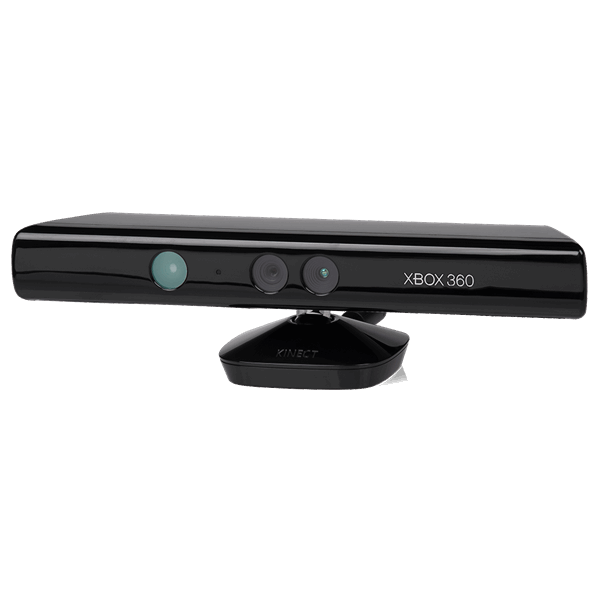
\includegraphics[width=0.3\textwidth]{./Imagenes/Bitmap/Kinect.png}
     }
     \hfill
\subfloat[PlayStation Move con Navigation Controller\label{septa4}]{%
       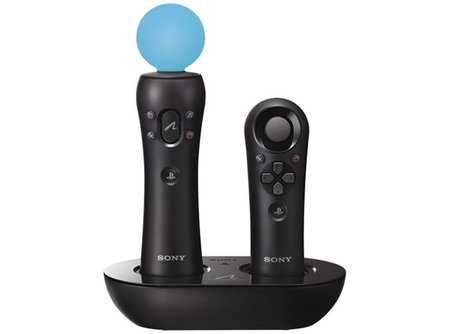
\includegraphics[width=0.3\textwidth]{./Imagenes/Bitmap/PSMove.jpg}
     }
\hfill
\subfloat[PlayStation Eye\label{septa5}]{%
       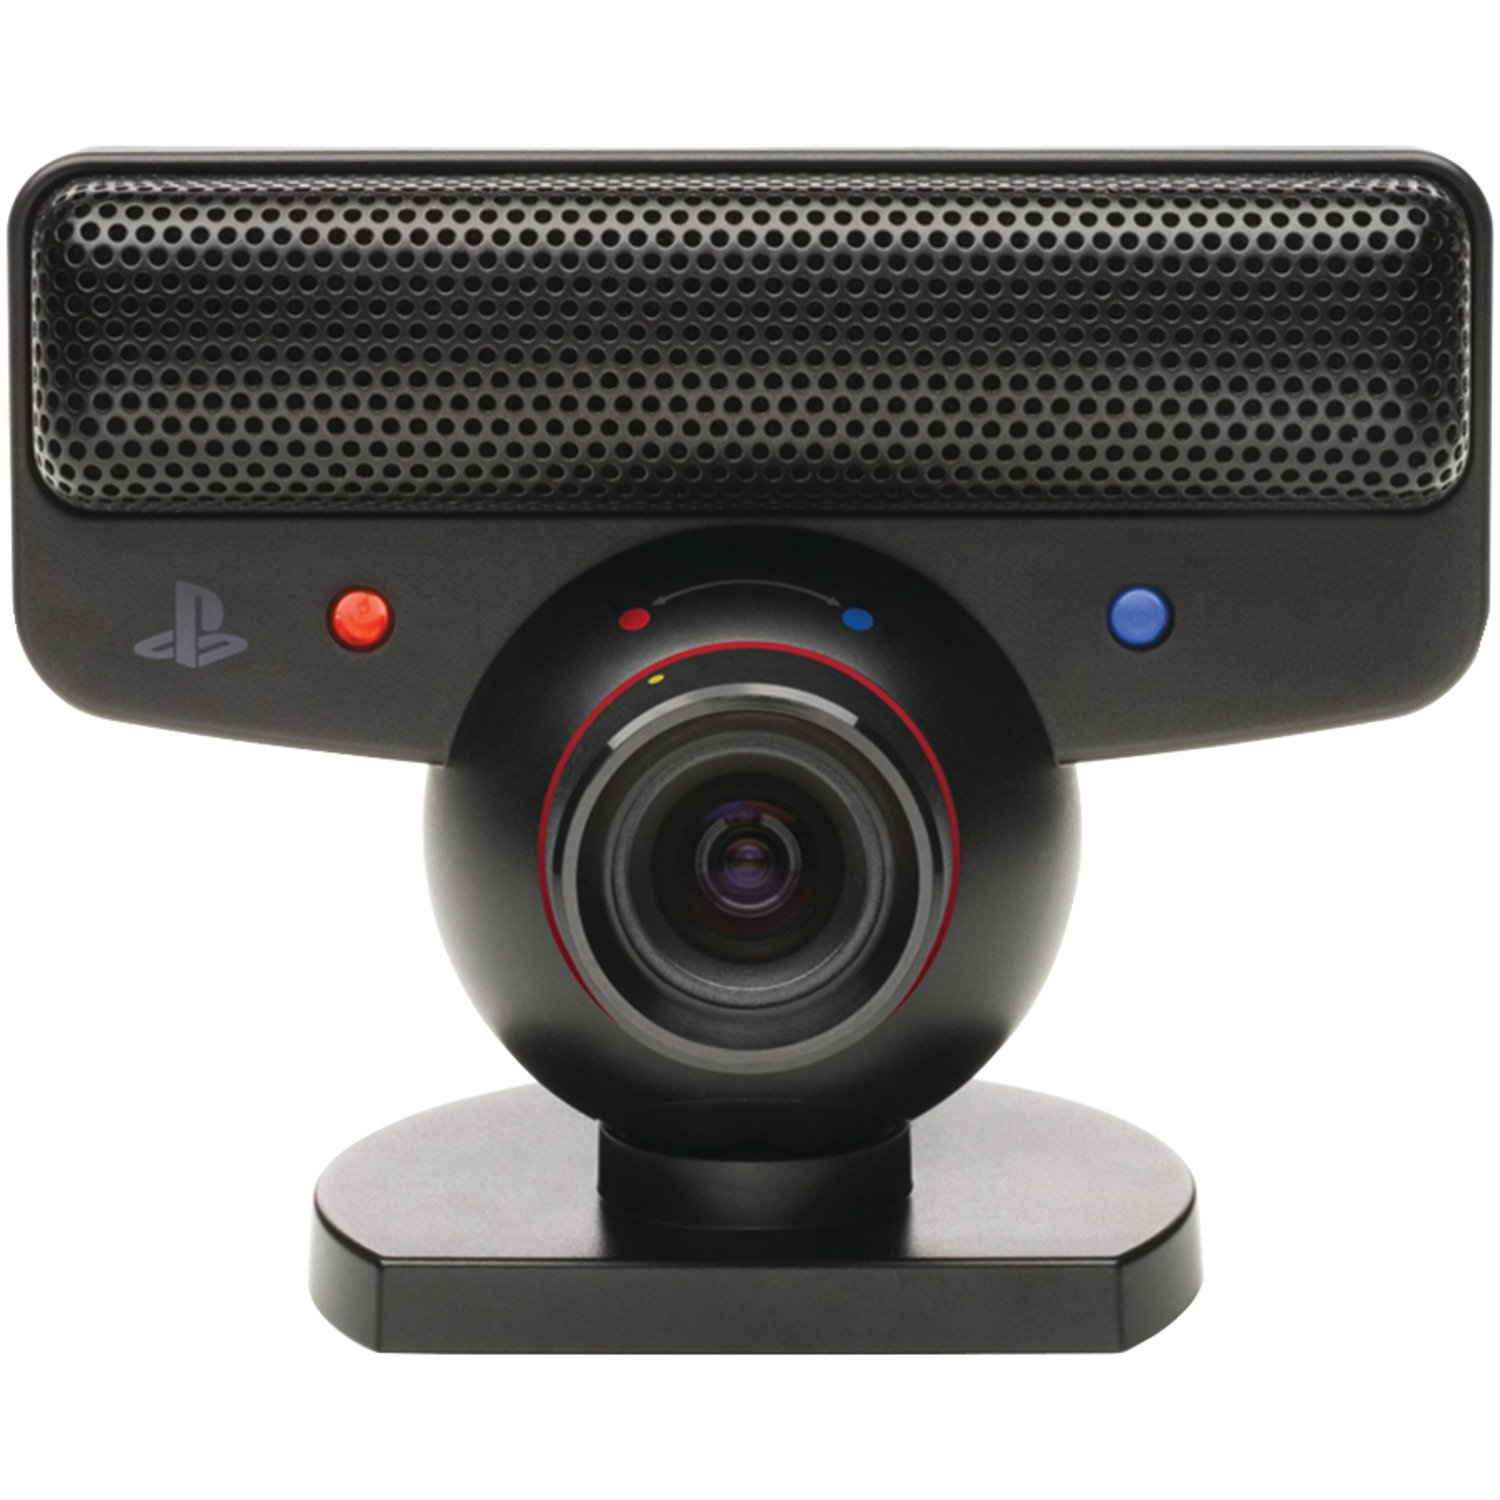
\includegraphics[width=0.3\textwidth]{./Imagenes/Bitmap/PSEye.jpg}
     }
     \caption{Dispositivos de entrada relevantes de Xbox y PlayStation en la 7"a  generaci\'on}
     \label{fig:septima2}
   \end{figure}

En 2010 Microsoft dio el salto a un nuevo controlador de videojuegos para su consola Xbox 360. Este nuevo perif\'erico es conocido con el nombre de \textbf{Kinect} (figura~\ref{septa3})\footnote{Im'agen extraida de \url{https://rb.gy/eoc6xq}} y permite a los usuarios controlar e interactuar con la consola sin necesidad de tener contacto f\'isico con un mando tradicional. Este control se realiza por gestos y reconocimiento de voz. El sensor Kinect es una barra horizontal de unas 9 pulgadas conectada a una peque\~na base circular con un eje que permite que esta rote. Adem\'as, est\'a dise\~nado para ser colocado por encima o por debajo de la televisi\'on. El dispositivo cuenta con una c\'amara RGB, un sensor de profundidad, un micr\'ofono de m\'ultiples matrices y un procesador personalizado que ejecuta el software patentado. Esto proporciona captura de movimiento de todo el cuerpo en 3D, reconocimiento facial y capacidades de reconocimiento de voz. El micr\'ofono de matrices del sensor de Kinect permite a la Xbox 360 llevar a cabo la localizaci\'on de la fuente ac\'ustica y la supresi\'on del ruido ambiente, permitiendo participar en el chat de Xbox Live sin utilizar auriculares. El sensor de profundidad es un proyector de infrarrojos combinado con un sensor CMOS monocromo que permite a Kinect ver la habitaci\'on en 3D en cualquier condici\'on de luz ambiental. El rango de detecci\'on de la profundidad del sensor es ajustable gracias al software de Kinect capaz de calibrar autom\'aticamente el sensor, basado en la jugabilidad y en el ambiente f\'isico del jugador, tal como la presencia de sof\'as, mesas y otro tipo de muebles.\\

PlayStation tambi\'en lanz\'o al mercado su sistema de control de videojuegos por movimiento, \textbf{PlayStation Move} (figura~\ref{septa4})\footnote{Im'agen extraida de \url{https://rb.gy/qvujth}}, y es compatible con los sistemas PS3 y PS4. PlayStation Move compiti\'o tanto con el Kinect de Xbox como con el WiiMote de Nintendo. Para poder utilizar PlayStation Move se necesitan 3 componentes: \textit{Motion Controller, Navigation Controller y PlayStation Eye} (figuras~\ref{septa4} y \ref{septa5}).\footnote{Im'agen extraida de \url{https://rb.gy/ls8cx6}} Motion Controller es el mando principal y tiene una forma alarga con una esfera luminosa en su parte superior. Esta esfera es utilizada para que PlayStation Eye detecte el mando. Esta c\'amara lee los movimientos del mando para posteriormente ser interpretados por el juego. Como complemento al Motion Controller, existe el Navigation Controller. Este controlador cumple la misma funci\'on que el Nunchuck de Wii. \\

%%%%%%%%%%%%%%%%%%%%%%%%%%%%%%%%%%%%%%%%%%%%%%%%%%%%%%%%%%%%%%%%%%

\subsection{Octava generaci\'on (2012-2020)}

Coincidiendo con la salida al mercado del PlayStation Move, Nintendo lanz\'o su nueva consola en 2012; la \textbf{Wii U} y con ella un controlador de videojuegos h\'ibrido. Este controlador h\'ibrido es el \textbf{Wii U GamePad} y es el mando principal de la consola. La principal distinci\'on con respecto a los mandos tradicionales es la incorporaci\'on de una pantalla t\'actil (figura~\ref{octava1}),\footnote{Im'agen extraida de \url{https://es.wikipedia.org/wiki/Wii_U}} la cual se utiliza para mostrar informaci\'on adicional durante una partida y adem\'as puede usarse como pantalla principal en caso de no disponer de un televisor mientras se juega. Adem\'as de como controlador de videojuegos, el Wii U GamePad es utilizado como control remoto independiente para controlar la pantalla de la televisi\'on u otro aparato v\'ia infrarrojos sin necesidad de tener la consola encendida. El mando contaba con altavoces y micr\'ofono e incorporaba una c\'amara frontal de 1.3 megapixeles. Los sensores que incorporaba eran: aceler\'ometro, giroscopio, geomagn\'etico e infrarrojo e incorporaba vibraci\'on. La conexi\'on a la consola se hac\'ia mediante bluetooth  y dispon\'ia de NFC para futuros accesorios que incorporaron a los diferentes videojuegos.\\

\begin{figure}[t]
     \subfloat[Wii U Gamepad\label{octava1}]{%
       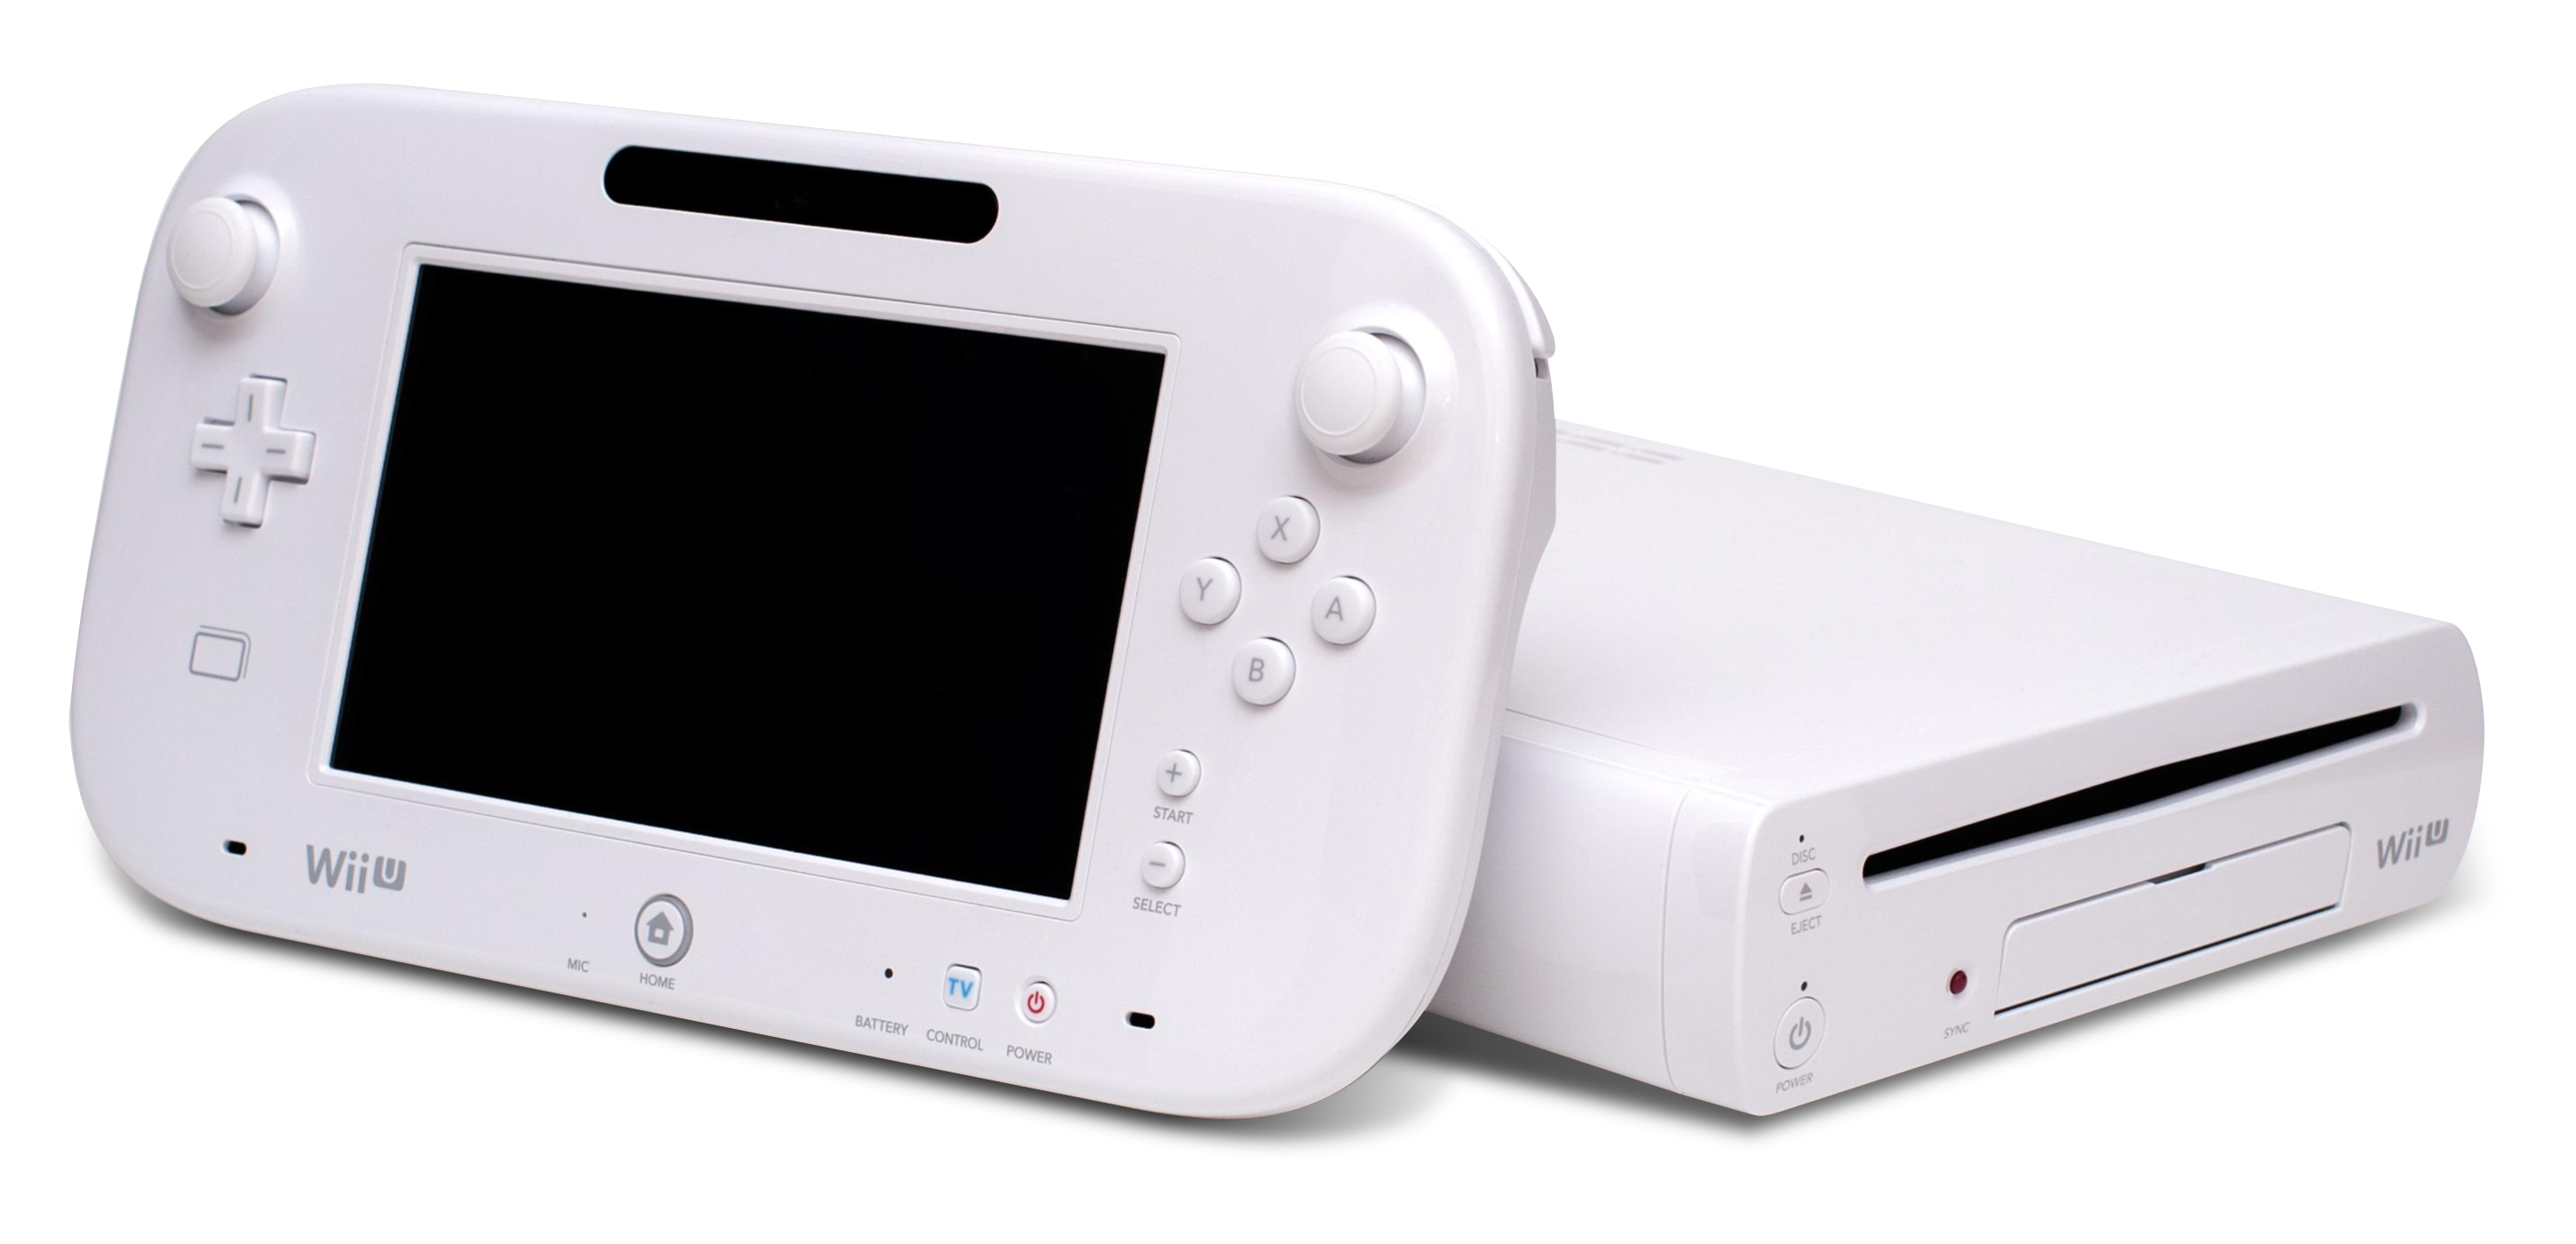
\includegraphics[width=0.3\textwidth]{./Imagenes/Bitmap/Wii_U_Console_and_Gamepad.png}
     }
     \hfill
\subfloat[Dualshock 4\label{octava2}]{%
       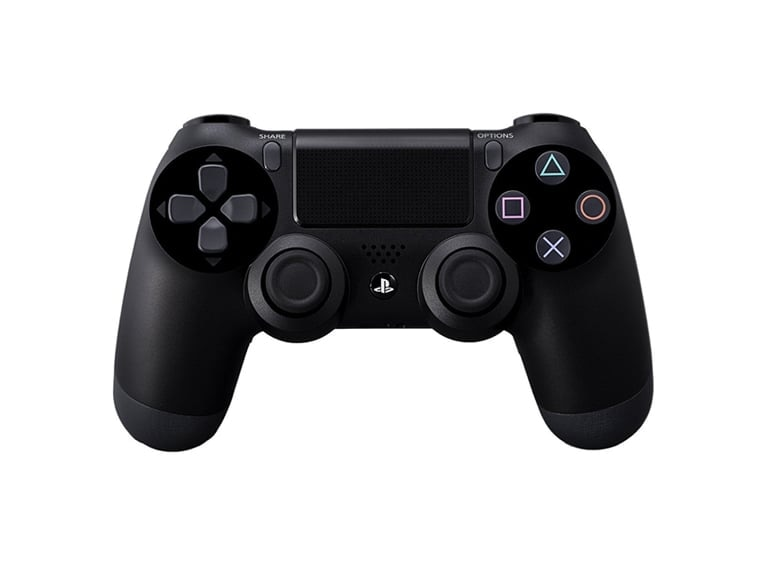
\includegraphics[width=0.3\textwidth]{./Imagenes/Bitmap/Dualshock4.jpg}
     }
\hfill
\subfloat[Xbox One Elite Controller\label{octava3}]{%
       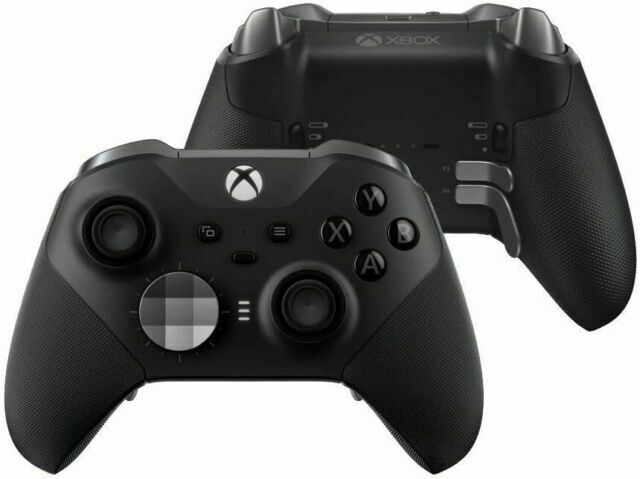
\includegraphics[width=0.3\textwidth]{./Imagenes/Bitmap/Xbox One Elite Controller.jpg}
     }
     \caption{Dispositivos de entrada relevantes en la 8"a  generaci\'on}
     \label{fig:octava}
   \end{figure}

En 2013 Sony hizo una revisi\'on de su DualShock y como mando de la consola PlayStation 4 lanz\'o el \textbf{DualShock 4} (figura~\ref{octava2}).\footnote{Im'agen extraida de \url{https://rb.gy/fuqos5}} Este mando a\~nadi\'o al dise\~no anterior un panel t\'actil en la parte frontal, lo que hizo que la distribuci\'on de los botones que antes eran centrales cambiasen. En la parte trasera se a\~nadi\'o una barra LED que se ilumina en varios colores para diferenciar e identificar a los diferentes jugadores. Microsoft por su parte en 2015 puso a la venta su nuevo \textbf{Xbox One Elite Controller}. Una de las principales caracter\'isticas es que tiene un dise\~no modular por lo que cada pieza es intercambiable para que cada jugador pueda adaptarlo a su medida. La personalizaci\'on es el principal aliciente en este mando ya que permite reprogramar tanto los cuatro botones tradicionales de la parte frontal como los gatillos. Tambi\'en se da la posibilidad de establecer curvas de sensibilidad en las palancas anal\'ogicas. Gracias a la posibilidad de a\~nadir piezas, este mando incluye 4 palancas m\'as en la parte trasera como puede verse en la figura~ \ref{octava3}.\footnote{Im'agen extraida de \url{https://rb.gy/5pyfl7}}\\

\begin{figure}[t]

\subfloat[Nintendo Switch\label{octava5}]{%
       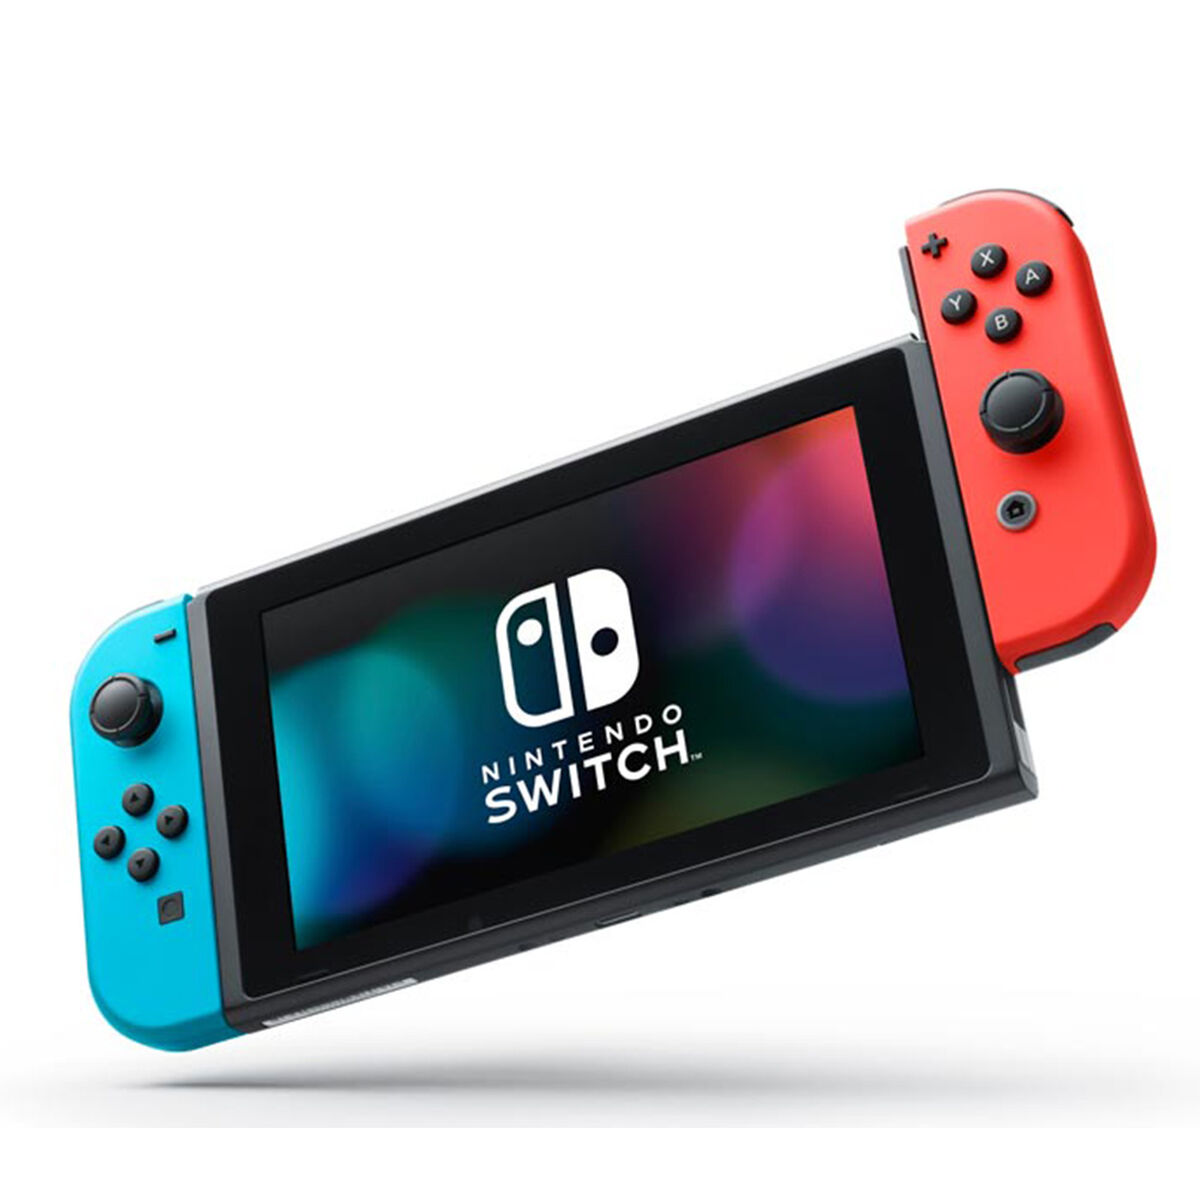
\includegraphics[width=0.4\textwidth]{./Imagenes/Bitmap/switch.jpg}
     }
 \hfill
     \subfloat[Par de Joy-Cons desacoplados\label{octava4}]{%
       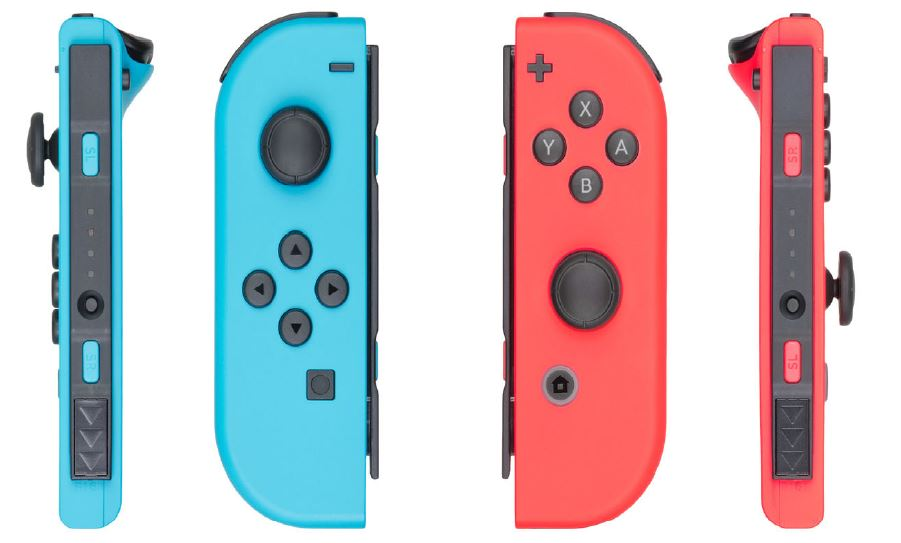
\includegraphics[width=0.5\textwidth]{./Imagenes/Bitmap/Joy-Con.jpg}
     }
    
     \caption{Nintendo Switch}
     \label{fig:octava2}
   \end{figure}

En 2016 Nintendo present\'o su nueva consola h\'ibrida que que tiene como base Wii U. La consola es \textbf{Nintendo Switch} (figura~\ref{octava5})\footnote{Im'agen extraida de \url{https://rb.gy/dpwawq}} y es una consola que puede ser jugada tanto de manera port\'atil como en formato sobremesa con una televisi\'on o un monitor. Los mandos dise\~nados para esta consola son los \textbf{Joy Con} y consisten en 2 unidades, cada uno de ellos contiene una palanca anal\'ogica y una matriz de botones. Estos mandos tienen la peculiaridad de que pueden usarse tanto acoplados a la consola o por separado. Cada uno de los Joy-Con puede ser utilizado como mando individual y se distribuyen en pares, designados como Joy-Con L y Joy-Con R. Una misma Nintendo Switch puede tener conectados hasta un total de 8 Joy-Con para juegos multijugador.\\

La comunicaci\'on que tienen los mandos con la consola se realiza por bluetooth gracias a una bater\'ia no extra\'ible de 525 mAh en cada mando. Ambos controladores contienen una palanca anal\'ogica, cuatro botones en su parte frontal, dos botones superiores, dos botones laterales accesibles cuando se desacoplan de la consola, un bot\'on - para el Joy-Con L y un bot\'on + para el Joy-Con R y un indicador de jugador luces LED (figura~\ref{octava4}). Cada uno de los Joy-Con contiene un aceler\'ometro y un giroscopio, que pueden ser utilizados para los juegos que incluyen movimiento. Adem\'as, el Joy-Con R contiene un sensor de seguimiento de profundidad infrarroja, que puede leer objetos y movimientos sostenidos delante de \'el. Junto con estas funcionalidades, el Joy-Con R dispone de un lector NFC. Cada uno de los Joy-Con incorpora un motor para hacer vibrar el mando durante las sesiones de juego.\\

Tambi\'en durante 2017, Sony anunci\'o una serie de juegos nuevos que se jugar\'ian de una forma totalmente diferente ya que el mando utilizado ser\'ia cada uno de los tel\'efonos m\'oviles de los usuarios. A esta serie de juegos se la conoce como \textbf{PlayLink}. La idea detr\'as de PlayLink es que todos los usuarios de la consola PlayStation 4 y sus familiares y amigos disponen de un dispositivo m\'ovil pero no todos disponen de varios mandos para poder jugar con m\'as personas en juegos cooperativos. PlayLink es una aplicaci\'on m\'ovil que cada usuario se descarga en su Android o iOS y as\'i puede usar su tel\'efono como un mando m\'as de PlayStation 4. El requisito para que la conexi\'on sea efectiva es que tanto la consola PS4 como los dispositivos m\'oviles que se vayan a usar est\'en conectados a la misma red WIFI.\\

%%%%%%%%%%%%%%%%%%%%%%%%%%%%%%%%%%%%%%%%%%%%%%%%%%%%%%%%%%%%%%%%%%

\subsection{Novena generaci\'on (2020-Actual)}

\begin{figure}[t]
\centering
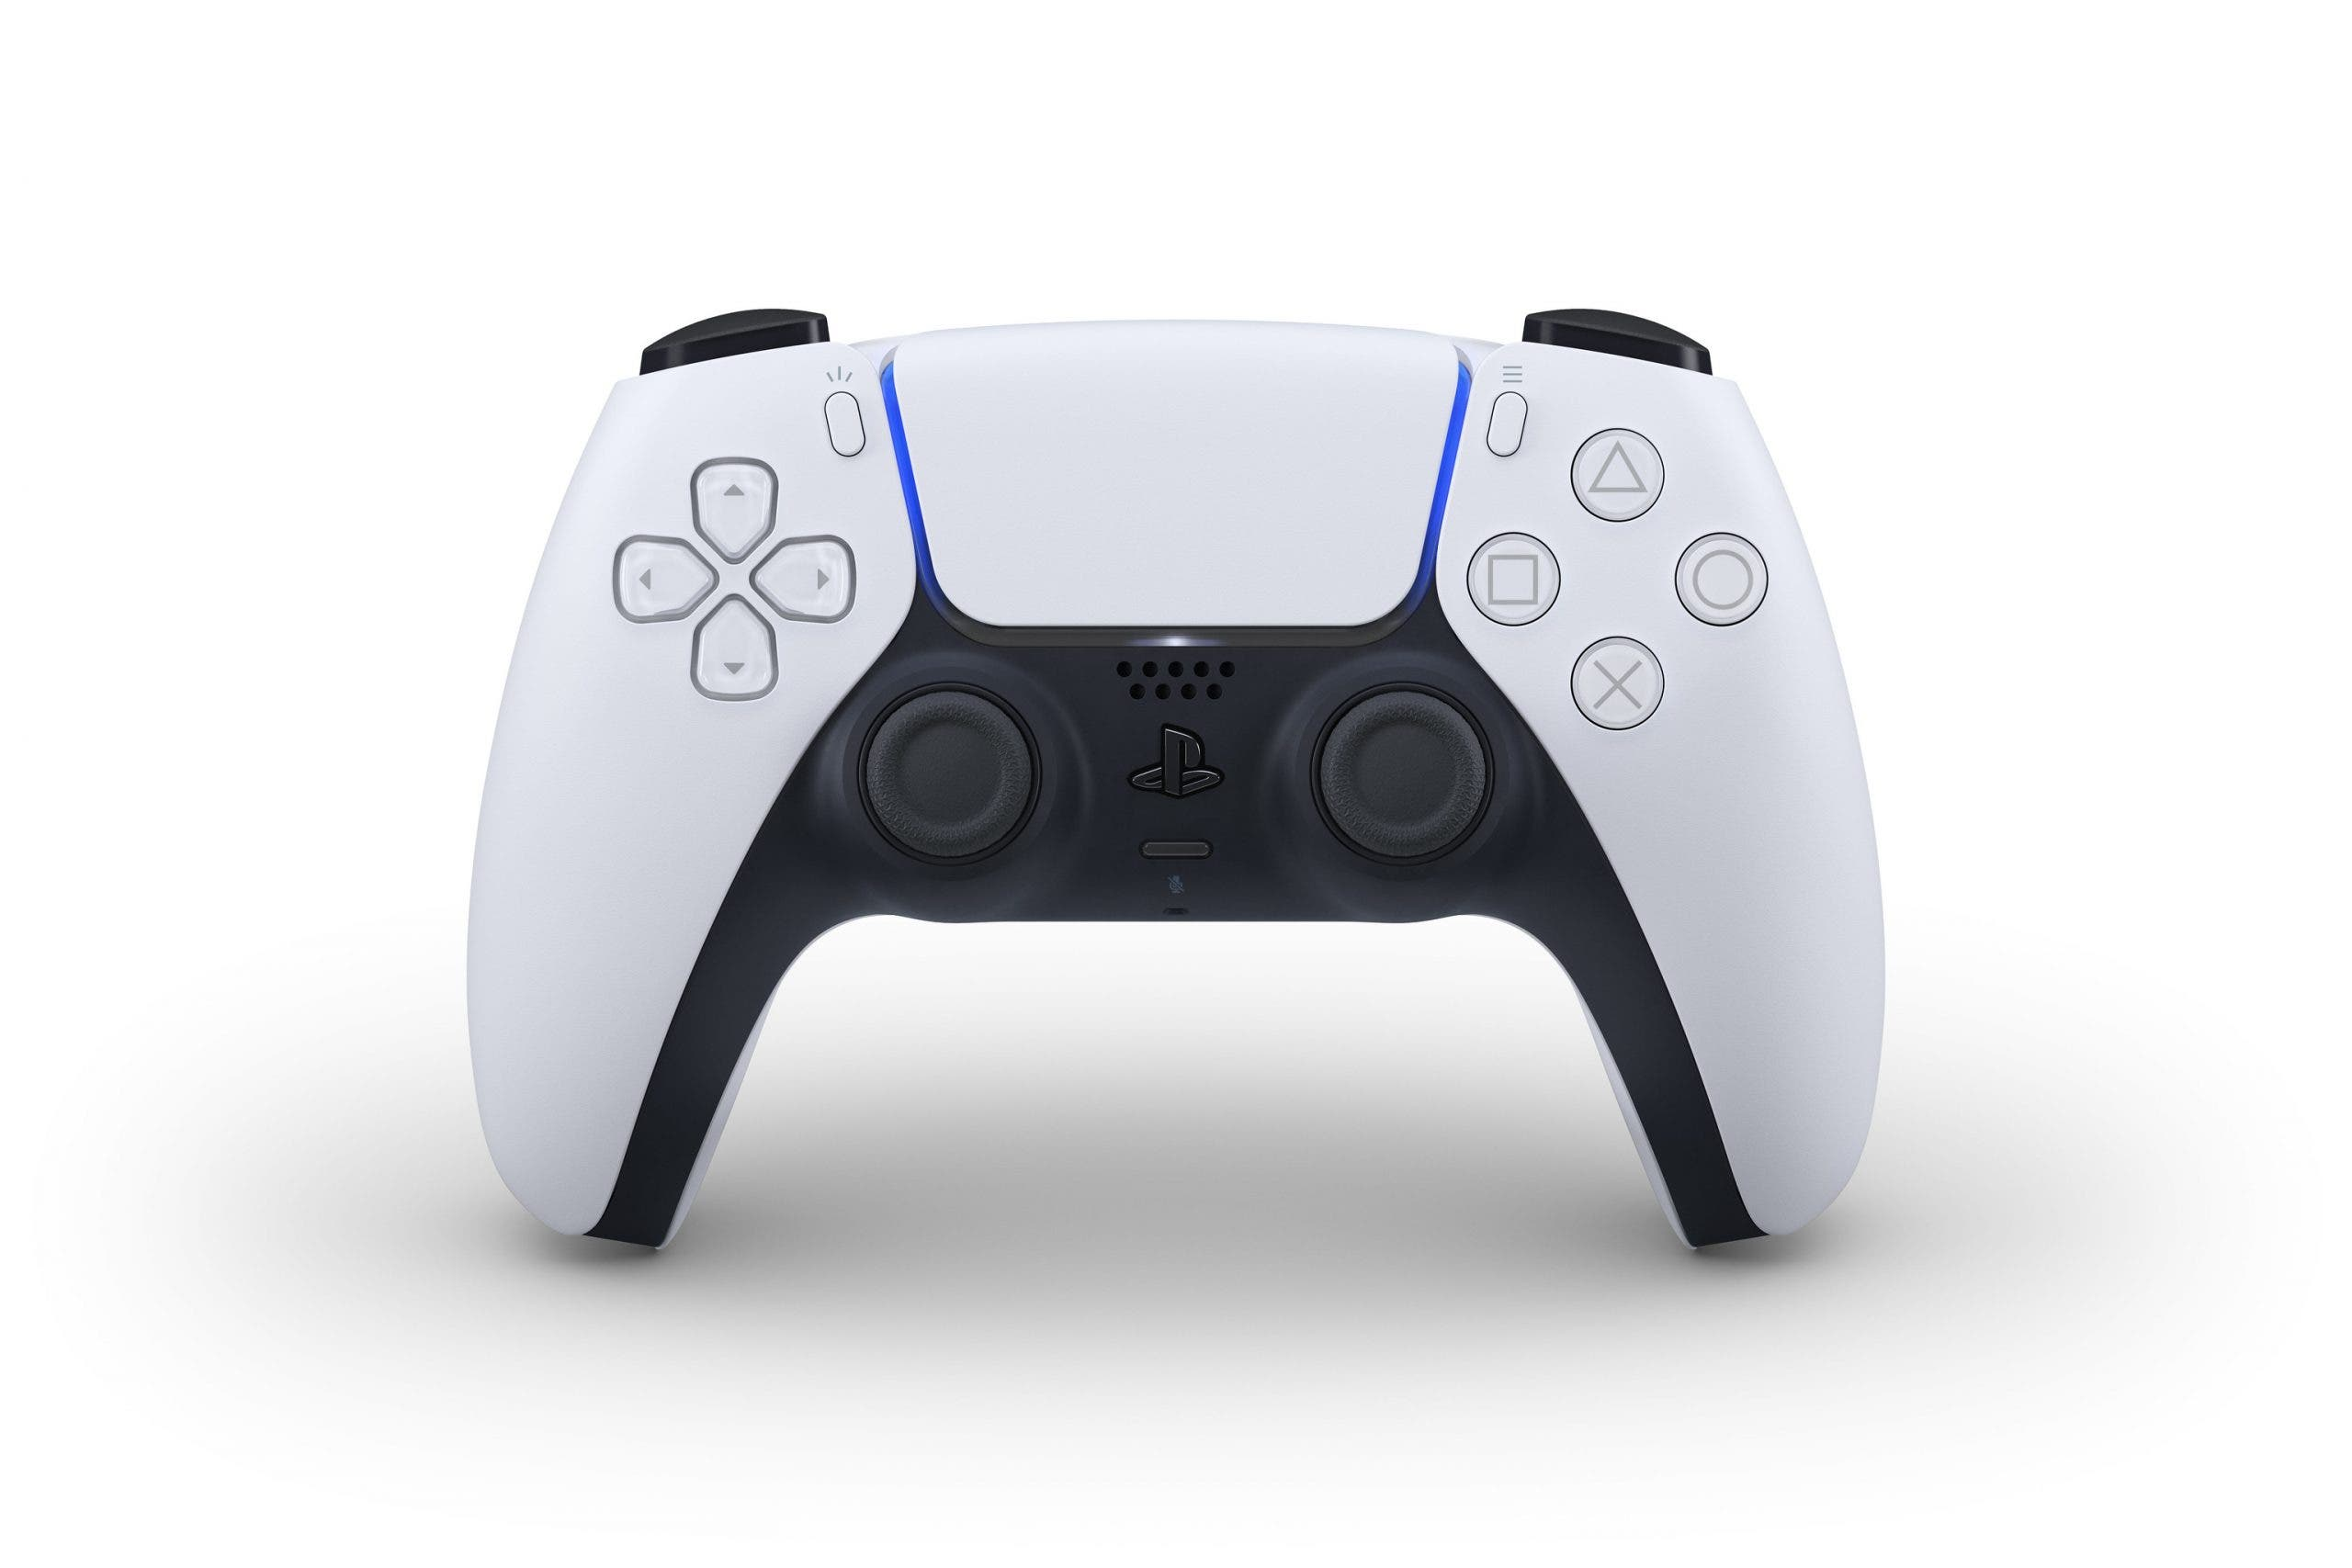
\includegraphics[width=0.4\textwidth]{./Imagenes/Bitmap/dualsense.jpg}
\caption{PS5 Dualsense Controller}
\label{Fig:dualsense}
\end{figure}

A finales del a\~no 2020 Sony lanz\'o al mercado su nueva consola, la PS5 y con ella un nuevo mando al que bautizaron como \textbf{DualSense} (figura~\ref{Fig:dualsense}).\footnote{Im'agen extraida de \url{https://rb.gy/36ofhk}} Como ya pasaba con el DualShock 4, este mando funciona con bater\'ia y lleva un altavoz integrado. La gran novedad que trae este mando es la retroalimentaci\'on h\'aptica. Se han sustituido los motores de vibraci\'on tradicionales por 2 activadores que emiten vibraciones din\'amicas capaces de simular todo tipo de sensaciones. Adem\'as de la nueva retroalimentaci\'on h\'aptica, el nuevo DualSense incorpora 2 gatillos adaptativos. Estos gatillos emiten diferente fuerza de resistencia contra el jugador dependiendo del arma que se est\'e utilizando. El ejemplo que pusieron los desarrolladores de Sony fue con la cuerda de un arco, inicialmente no tiene resistencia pero cuanto m\'as se tense la cuerda del arco m\'as fuerza es necesaria.

\section{\textit{Feedback} en los controladores}

En los inicios de los videojuegos y de las consolas el objetivo fue la creaci\'on de nuevos tipos de juegos con diferentes mec\'anicas y mejoras gr\'aficas. En la era actual de los videojuegos se ha ido mucho m\'as lejos de los primeros juegos como Pong y Tetris, la tendencia ha llevado a la creaci\'on de escenarios virtuales m\'as realistas y a que el jugador formase parte de ese entorno virtual. Particularmente la respuesta que se da al usuario del videojuego al realizar acciones es conocida como \textbf{tecnolog\'ia h\'aptica}. Este tipo de tecnolog\'ia se refiere al conjunto de interfaces tecnol\'ogicos que interaccionan con una persona mediante el sentido del tacto. La tecnolog\'ia h\'aptica tiene sus inicios en los dispositivos de los sistemas servo para controlar grandes aviones con la intenci\'on de poder hacerlo de manera remota. En estos sistemas se instal\'o un sistema de control que proporcionaba una resistencia a la palanca del piloto proporcional al \'angulo de ataque del avi\'on. Otro ejemplo destacable de esta tecnolog\'ia se encuentra en la pel\'icula \textbf{4-D Honey, I Shrunk the Audience!}\footnote{https://screencrush.com/honey-i-shrunk-the-audience-horror-film/} del a\~no 1994 que simulaba que los ratones se soltaban por el auditorio y corr\'ian por toda la sala. Para conseguir esta simulaci\'on se bombeaba aire a trav\'es de un peque\~no tubo de pl\'astico y al agitarse, imitaba la sensaci\'on de las colas de los ratones rozando las piernas de los espectadores. \\

En los videojuegos esta tecnolog\'ia fue introducida a trav\'es de los controladores. Al inicio estos sistemas de vibraci\'on se introdujeron en los controladores como dispositivos que se acoplaban al mando por separado como pasaba con el \textbf{Rumble Pack} de Nintendo 64. Con la salida del \textbf{Dualshock} en su versi\'on japonesa esto cambi\'o. Este mando incorporaba un sistema de vibraci\'on conocido como \textit{tabletas vibradoras (rumble packs)} que ten\'ian ese efecto de vibraci\'on al conducir veh\'iculos o disparar armas de fuego. Con la llegada de las pantallas t\'actiles tambi\'en aparecieron las pantallas h\'apticas. Estas pantallas son aquellas que transmiten una vibraci\'on al tocarla. El ejemplo m\'as actual de tecnolog\'ia h\'aptica puede encontrarse en la reciente consola de Nintendo, Nintendo Switch. Nintendo no ha denominado a la tecnolog\'ia que usan sus Joy-Cons como tecnolog\'ia h\'aptica sino como \textbf{Rumble HD}. \\

\begin{figure}[t]
     \subfloat[Force Feedback Pro\label{feedback1}]{%
       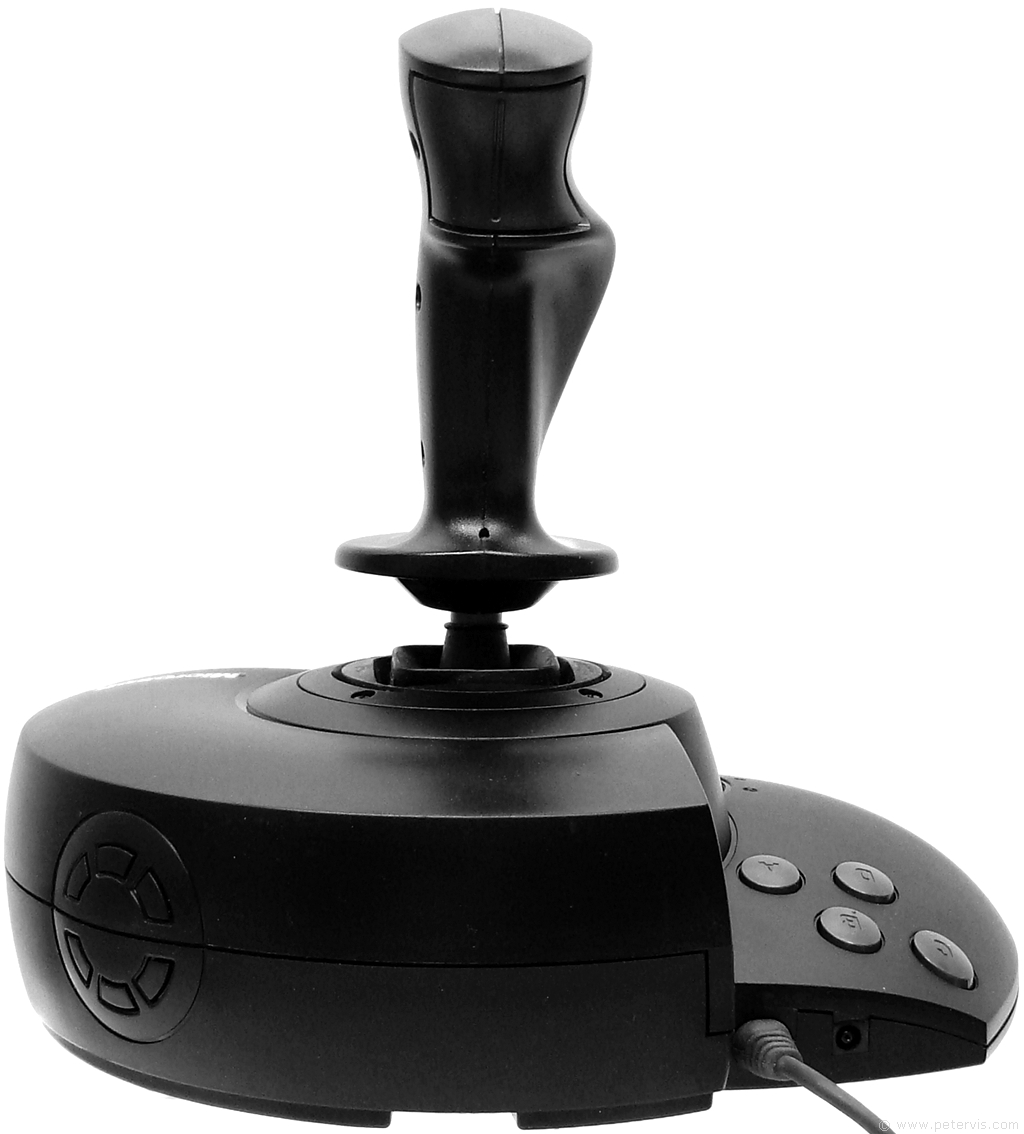
\includegraphics[width=0.4\textwidth]{./Imagenes/Bitmap/sidewinder-force-feedback-pro-back-view.jpg}
     }
     \hfill
\subfloat[Microsoft Sidewinder Force Feedback Wheel\label{feedback2}]{%
       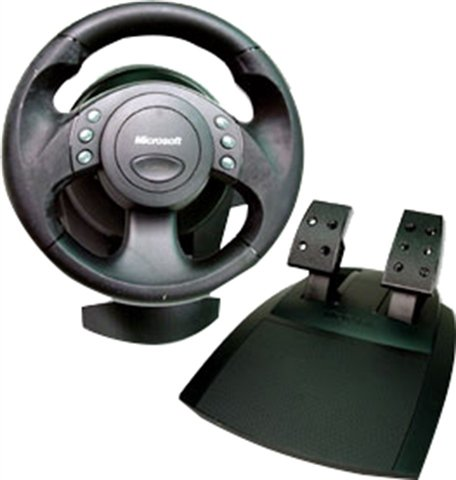
\includegraphics[width=0.4\textwidth]{./Imagenes/Bitmap/SACCMICFFW_l.jpg}
     }
     \caption{Primeros dispositivos con \textit{force feedback}}
     \label{fig:feedback}
   \end{figure}

El mundo de la simulaci\'on trata de intentar recrear el mundo real dentro de un videojuego. En este tipo de juegos de simulaci\'on la respuesta que recibe el usuario importa mucho debido al car\'acter inmersivo que puede llegar a ofrecer. Para lograr esto, en 1997 Microsoft sac\'o al mercado un producto que inclu\'ia \textit{force feedback}, Force Feedback Pro (figura~\ref{feedback1}).\footnote{Im'agen extraida de \url{https://rb.gy/9kgubs}} Para realizar la comunicaci\'on entre el PC y el dispositivo se utilizaba un puerto MIDI. Este puerto MIDI ven\'ia incluido en las tarjetas de sonido que los usuarios compraban para tener un mejor sonido a la hora de jugar a videojuegos. El feedback era mandado al dispositivo de la misma manera en la que se enviaban notas musicales a los instrumentos MIDI pero el dispositivo de \textit{feedback} reproduc\'ia vibraciones en lugar de notas. En ese mismo a\~no, Microsoft sac\'o al mercado el que ser\'ia el primer volante con retroalimentaci\'on (figura~\ref{feedback2}).\footnote{Im'agen extraida de \url{https://rb.gy/ajprge}} Este ser\'ia el primer volante para jugar fuera de las m\'aquinas recreativas arcade.\\



\section{Sistemas de \textit{streaming} en videojuegos}

Con la extensi\'on de los dispositivos m\'oviles en el mundo de los videojuegos y las mejoras en las conexiones a Internet, la industria de los videojuegos se mueve a pasos acelerados hacia el \textit{gaming} en la nube. Servicios de retransmisi\'on v\'ia streaming como \textit{Netflix} o \textit{Amazon Prime Video} ofrecen la posibilidad de disponer de un cat\'alogo de series y pel\'iculas a trav\'es de Internet. Con este precedente, empresas como Google\footnote{https://stadia.google.com/} y Nvidia\footnote{https://www.nvidia.com/es-es/geforce-now/} se han adentrado en el mundo de los juegos en la nube.\\

Esta nueva forma no solamente consiste en retransmitir al usuario final a la partida que est\'a jugando sino que el proceso va mucho m\'as all\'a. Esta diferencia tiene lugar a la hora de tratar la entrada del usuario. En un videojuego tradicional, ejecutado en la misma m\'aquina en la que se est\'a jugando, una vez el usuario realiza una entrada el videojuego lo procesa y genera una respuesta apropiada. En los videojuegos en la nube una vez que el usuario realiza una acci\'on, \'esta debe ser enviada al servidor donde el juego est\'a siendo ejecutado. Una vez en el servidor, la entrada que gener\'o el usuario es tratada y se realizan los cambios en el estado del juego que haya provocado el usuario con su entrada. Cuando el estado cambia en el servidor se prepara el frame, se codifica y es enviado de vuelta al usuario que tendr\'a que decodificar el frame una vez le llegue al dispositivo donde est\'e jugando \citep{cloudgaming}.

Los anchos de banda requeridos para estas dos tecnolog\'ias var\'ian con las resoluciones a las que se quiera jugar (tabla~\ref{stadiovsgeforce}). Ambos sistemas aconsejan una conexi\'on Ethernet o un router que disponga de una red de frecuencia 5 GHz.

\begin{table}[h]
\centering
    \begin{tabular}{lll}
        \toprule
         & \textbf{Google Stadia} & \textbf{Nvidia GeForce Now} \\
        \midrule
        \textbf{720p 60fps} & 10 Mbps & 15 Mbps\\
        \textbf{1080p 60fps} & 20 Mbps & 25 Mbps \\
		\textbf{4K 60fps} & 35Mbps & No Disponible \\
        \bottomrule
    \end{tabular}
\caption{Ancho de banda necesario para jugar a Stadia vs GeForce Now}
\label{stadiovsgeforce}
\end{table}


En los sistemas de streaming de video convencionales se utiliza la t\'ecnica conocida como \textit{buffering}. Esta t\'ecnica puede realizarse siempre y cuando la conexi\'on a Internet sea lo suficientemente r\'apida como para descargar un fragmento de los datos que van a usarse a continuaci\'on antes de necesitarlos. Con esto lo que se consigue es aprovechar los momentos en los que se dispone de un ancho de banda mayor para descargar parte del contenido que se va a visualizar a continuaci\'on. Esto permite al usuario no ser consciente de retrasos moment\'aneos en la red. En el mundo de los juegos en la nube este proceso se ve truncado por la interacci\'on del usuario. El juego no puede predecir lo que va a pasar por lo que no se puede hacer \textit{buffering} de los frames. Este hecho convierte a los sistemas de juegos en la nube en sistemas sensibles a los retrasos en la red.\\

\begin{figure}[h]

\centering
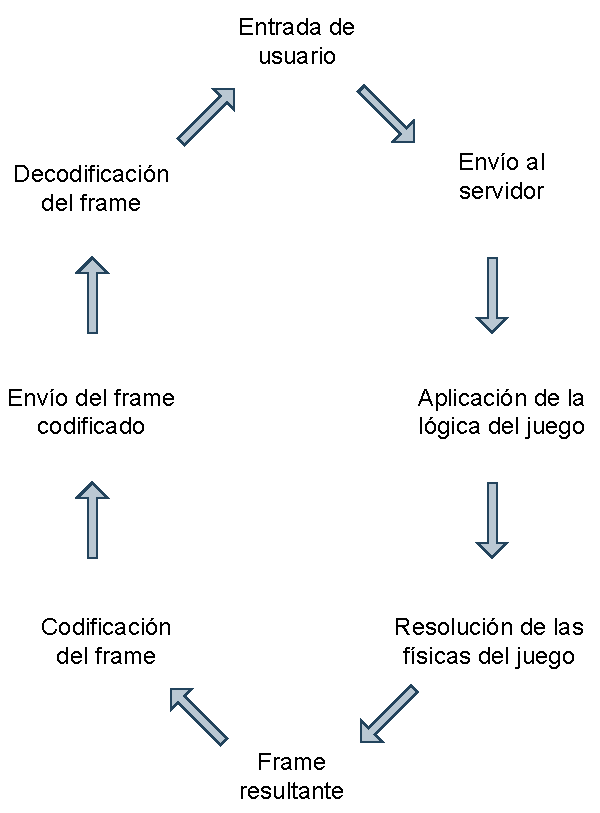
\includegraphics[width=0.6\textwidth]{./Imagenes/Vectorial/cloudgaming cycle.pdf}
\caption{Flujo de la entrada de usuario de juegos en la nube}
\label{cycle}
\end{figure}

En los juegos que se transmiten por red, una vez que el usuario ha realizado la pulsaci\'on, esta pulsaci\'on es transmitida al servidor de manera segura. Una vez que la entrada del usuario llega al servidor, debe ser desencriptada y los cambios deben aplicarse en el juego. Una vez aplicados los cambios, el frame debe ser codificado y transmitido de vuelta al usuario. El usuario decodifica el frame y lo muestra. Este ciclo se repite constantemente en el ciclo de los juegos en la nube (ver figura~\ref{cycle}).\\

El inter\'es de los jugadores por un producto depende de muchos aspectos. Uno de los principales es la experiencia que el usuario recibe al jugar. Esto hace que una ca\'ida del servicio mientras el jugador est\'a jugando puede crear una frustraci\'on en el usuario y hacer que este pierda el inter\'es. La latencia est\'a definida como el tiempo de respuesta entre el servidor donde se est\'a ejecutando el juego y el cliente que est\'a jugando. Existen diferentes tipos de latencias o retrasos en la red. El m\'as com\'un es el retraso en la renderizaci\'on del siguiente frame. \\

En este proyecto todos estos inconvenientes convergen. El uso de la red requiere de un m\'inimo ancho de banda y es por esto que tal y como se hablaba al principio del cap\'itulo, los sistemas como Stadia piden unas m\'inimas velocidades para poder asegurar la fluidez a la hora de jugar. Un juego que ejecute a 60 frames por segundo quiere decir que se disponen de 16 milisegundos aproximadamente para realizar el ciclo comentado en la figura~\ref{cycle}. En ocasiones para conseguir mantener estas tasas de frames se realiza una disminuci\'on de la calidad gr\'afica con la que llega el frame. Realizar estos cambios din\'amicos de manera puntual en picos donde el uso del ancho de banda es demasiado ayuda a que el jugador no tenga desconexiones o retrasos en la entrada que ha realizado.\\

\bigskip
\Large{\textbf{En el pr\'oximo cap\'itulo}}\\
\normalsize

Tal y como hemos podido ver en este cap\'itulo, a lo largo de la historia los controladores de videojuegos han ido agregando elementos h\'apticos, ergon\'omicos y sonoros para mejorar la experiencia de los usuarios. Con los nuevos sistemas de \textit{cloud gaming} se ha a\~nadido mucha m\'as versatilidad a la hora de jugar pero esta opci\'on tiene unos costes. En el pr\'oximo cap\'itulo se explicar\'an las diferentes alternativas y decisiones tomadas a la hora de realizar el protocolo de comunicaci\'on para el control de un videojuego con un dispositivo m\'ovil.


%-------------------------------------------------------------------


% Variable local para emacs, para  que encuentre el fichero maestro de
% compilaci�n y funcionen mejor algunas teclas r�pidas de AucTeX
%%%
%%% Local Variables:
%%% mode: latex
%%% TeX-master: "../ManualTeXiS.tex"
%%% End:

%---------------------------------------------------------------------
%
%                          Cap�tulo 3
%
%---------------------------------------------------------------------
%
% 03Edicion.tex
% Copyright 2009 Marco Antonio Gomez-Martin, Pedro Pablo Gomez-Martin
%
% This file belongs to the TeXiS manual, a LaTeX template for writting
% Thesis and other documents. The complete last TeXiS package can
% be obtained from http://gaia.fdi.ucm.es/projects/texis/
%
% Although the TeXiS template itself is distributed under the 
% conditions of the LaTeX Project Public License
% (http://www.latex-project.org/lppl.txt), the manual content
% uses the CC-BY-SA license that stays that you are free:
%
%    - to share & to copy, distribute and transmit the work
%    - to remix and to adapt the work+
%
% under the following conditions:
%
%    - Attribution: you must attribute the work in the manner
%      specified by the author or licensor (but not in any way that
%      suggests that they endorse you or your use of the work).
%    - Share Alike: if you alter, transform, or build upon this
%      work, you may distribute the resulting work only under the
%      same, similar or a compatible license.
%
% The complete license is available in
% http://creativecommons.org/licenses/by-sa/3.0/legalcode
%
%---------------------------------------------------------------------


\begin{FraseCelebre}
\begin{Frase}
%Si quieres ser le�do m�s de una vez, no vaciles en borrar a menudo.
%Rem tene, verba sequentur (Si dominas el tema, las palabras vendr�n solas)
\end{Frase}
\begin{Fuente}
%Horacio
%Cat�n el Viejo
\end{Fuente}
\end{FraseCelebre}


\chapter{Especificaci\'on de la herramienta}
\label{cap3}
\label{cap:especificacion}

%-------------------------------------------------------------------
\section{Introducci\'on}
%-------------------------------------------------------------------
\label{cap3:sec:intro}
En este cap\'itulo se exponen las diferentes tecnolog\'ias involucradas en el proyecto y ver las decisiones tomadas en base a las necesidades para la realizaci\'on de este proyecto. La finalidad del proyecto es la conexi\'on entre 2 dispositivos, uno de ellos ejecuta el juego y el otro funciona como un dispositivo de entrada / mando para controlar el videojuego. 
Para conseguir esta comunicaci\'on entre ambos dispositivos es necesario plasmar la funcionalidad que se quiere dar y la posterior creaci\'on e implementaci\'on de un protocolo de red.


%-------------------------------------------------------------------
\section{Funcionalidad}
%-------------------------------------------------------------------

En los \'ultimos a\~nos se ha visto un aumento en la incorporaci\'on de elementos t\'actiles en los controladores de videojuegos. Empresas como Sony a\~nadieron una pantalla t\'actil en el Dualshock4, Nintendo con las consolas port\'atiles lleva varias generaciones a\~nadiendo pantallas t\'actiles a sus consolas y los dispositivos m\'oviles cada vez son m\'as usados para jugar a videojuegos.
Es por esto que en este proyecto, la comunicaci\'on entre 2 dispositivos ser\'a m\'as espec\'ifica y ser\'a entre un dispositivo en el cual se ejecuta el juego y un dispositivo m\'ovil que servir\'a como mando. Una de las principales diferencias entre un mando tradicional y un dispositivo m\'ovil es la pulsaci\'on de botones. El feedback recibido en la pulsaci\'on de una pantalla t\'actil es inexistente a no ser que no se especifique en la funcionalidad de la aplicaci\'on y debe ser lo suficientemente sutil como para no ser molesto a la hora de jugar.

Otras de las caracter\'sticas que tiene un dispositivo m\'ovil frente a un mando tradicional es el uso de gestos espec\'ificos. Una gran parte de estos gestos son utilizados de manera natural ya que son asociados al uso de dispositivos m\'oviles. 

Al usar un dispositivo m\'ovil, tenemos a nuestra disposici\'on una pantalla que nos permite a\~nadir im\'agenes, videos o incluso gameplay como lo hac\'ia Nintendo con su consola WiiU.

Con estas caracter\'isticas contempladas, las principales funcionalidades que debe tener este proyecto son:

\begin {itemize}
\item Env\'io de pulsaciones y gestos admisibles en pantallas t\'actiles.
\item Env\'io de im\'agenes est\'aticas.
\item Env\'io de im\'agenes de manera constante, simulando un streaming de video.
\item El uso de vibraci\'on como feedback de la pulsaci\'on de la pantalla.
\end {itemize}

%-------------------------------------------------------------------
\section{Protocolo de comunicaci\'on}
%-------------------------------------------------------------------

Un protocolo de comunicaci\'on es un sistema de reglas que permiten a 2 o m\'as dispositivos comunicarse entre ellos. En inform\'atica estas reglas se establecen para permitir la transmisi\'on de datos y la forma en la que la informaci\'on debe ser procesada. Cada mensaje tiene un significado exacto destinado a obtener una respuesta de un rango de posibles respuestas predeterminadas para esa situaci\'on en particular. Una de las caracter\'isticas principales de un protocolo de comunicaci\'on es que ambas partes tienen que acordar los mensajes que se van a enviar y a recibir. 

En este proyecto ambos dispositivos envian y reciben mensajes por lo que no puede definirse un servidor y un cliente, sin embargo se puede hacer una distinci\'on entre qui\'en env\'ia los botones que se han pulsado y qui\'en ejecuta el juego. El criterio utilizado para este proyecto ha sido el de un sistema \textbf{\textit{little-endian}}. Al inicio de la comunicaci\'on, el dispositivo encargado de ejecutar el juego debe quedarse a la escucha en un puerto asignado a la espera de un primer mensaje. El tama\~no de este mensaje es de 8 bytes y su estructura es la siguiente:

\begin {itemize}
\item Los 4 primeros bytes son un n\'umero de tipo \textit{int} que simboliza el ancho del dispositivo m\'ovil.
\item Los 4 \'ultimos bytes son un n\'umero de tipo \textit{int} que simboliza el alto del dispositivo m\'ovil.
\end {itemize}

\begin{table}[h!]
\centering
\begin{tabular}{|l|l|l|} 
\hline
Bits                    & 0-31                   & 32-63                   \\
\hline
\multicolumn{1}{|c|}{0} & \multicolumn{1}{c|}{Ancho} & \multicolumn{1}{c|}{Alto}  \\
\hline
\end{tabular}
\caption{Primer mensaje del controlador al ejecutor de juego}
\label{table:2}
\end{table}


La comprobaci\'on que se realiza en este mensaje es si se reciben 8 bytes en el lado del dispositivo que ejecuta el juego.

Una vez la conexi\'on se ha establecido correctamente, el dispositivo que ejecuta el juego env\'ia al controlador la duraci\'on de la vibraci\'on que debe realizar para que el usuario reciba un feedback h\'aptico. Este mensaje contiene un \textit{int} de 4 bytes que representa el tiempo que debe durar la vibraci\'on en milisegundos.

\begin{table}[h!]
\centering
\begin{tabular}{|l|c|} 
\hline
Bits                    & 0-31                 \\
\hline
\multicolumn{1}{|c|}{0} & Tiempo de vibraci\'on  \\
\hline
\end{tabular}
\caption{Tiempo de vibraci\'on del dispositivo movil en milisegundos}
\label{table:2}
\end{table}

Tras el env\'io de este mensaje comienza un bucle de juego en el que ambos dispositivos intercambian mensajes de una manera no ordenada. El dispositivo que se encarga de ejecutar el juego env\'ia los siguientes mensajes:
\begin {itemize}
\item En caso de que se decida enviar im\'agen de manera constante, ya sea en forma de streaming de video o una im\'agen est\'atica, esta im\'agen es comprimida en formato \textbf{\textit{PNG}}.
\item Se env\'ia el flag de vibraci\'on al controlador. Este flag es un \textit{int} de 4 bytes cuyo valor tiene que ser 0 para que vibre.
\end {itemize}

Adem\'as de enviar estos mensajes, el dispositivo encargado de ejecutar el juego recibir\'a mensajes de 9 bytes cada uno cuya estructura ser\'a:
\begin {itemize}
\item El primer byte es el tipo de la pulsaci\'on. El valor 0 indica el comienzo de la pulsaci\'on y el valor 1 indica el fin de la pulsaci\'on.
\item Los siguentes 4 bytes representan un \textit{int} cuyo valor indica la posici\'on X de la pantalla del dispositivo m\'ovil donde se ha pulsado el bot\'on.
\item Los \'ultimos 4 bytes representan un \textit{int} cuyo valor indica la posici\'on Y de la pantalla del dispositivo m\'ovil donde se ha pulsado el bot\'on.
\end {itemize}

\begin{table}[h!]
\centering
\begin{tabular}{|l|c|c|c|} 
\hline
Bits                    & 0-7               & 8-39                            & 40-71                            \\ 
\hline
\multicolumn{1}{|c|}{0} & Tipo de pulsaci\'on & \multicolumn{1}{l|}{Posici\'on X} & \multicolumn{1}{l|}{Posici\'on Y}  \\
\hline
\end{tabular}
\caption{Pulsaci\'on enviada desde el dispositivo m\'ovil al ejecutor del juego}
\label{table:2}
\end{table}

Para el cierre ordenado de la comunicaci\'on desde el dispositivo m\'ovil se env\'ia un mensaje de tama\~no 1 byte que tiene el valor 2. La recepci\'on de este mensaje hace que el dispositivo que ejecuta el juego env\'ie 1 byte con el valor 1 al dispositivo m\'oviles y ambos cierran la conexi\'on. Estos mensajes puedes enviarse y recibirse en cualquier momento en caso de que sucediese cualquier error durante la comunicaci\'on. Para la detecci\'on de una p\'erdida de conexi\'on entre el dispositivo m\'ovil y el dispositivo que ejecuta el juego, este dispone de un tiempo m\'aximo en el que si no se reciben mensajes se finaliza la conexi\'on (Time Out).

\begin {itemize}
\item \textbf{TODO:}Diagrama del protocolo con explici\'on.
\end {itemize}



% Variable local para emacs, para  que encuentre el fichero maestro de
% compilaci�n y funcionen mejor algunas teclas r�pidas de AucTeX
%%%
%%% Local Variables:
%%% mode: latex
%%% TeX-master: "../ManualTeXiS.tex"
%%% End:

%%---------------------------------------------------------------------
%
%                          Parte 2
%
%---------------------------------------------------------------------
%
% Parte2.tex
% Copyright 2009 Marco Antonio Gomez-Martin, Pedro Pablo Gomez-Martin
%
% This file belongs to the TeXiS manual, a LaTeX template for writting
% Thesis and other documents. The complete last TeXiS package can
% be obtained from http://gaia.fdi.ucm.es/projects/texis/
%
% Although the TeXiS template itself is distributed under the 
% conditions of the LaTeX Project Public License
% (http://www.latex-project.org/lppl.txt), the manual content
% uses the CC-BY-SA license that stays that you are free:
%
%    - to share & to copy, distribute and transmit the work
%    - to remix and to adapt the work
%
% under the following conditions:
%
%    - Attribution: you must attribute the work in the manner
%      specified by the author or licensor (but not in any way that
%      suggests that they endorse you or your use of the work).
%    - Share Alike: if you alter, transform, or build upon this
%      work, you may distribute the resulting work only under the
%      same, similar or a compatible license.
%
% The complete license is available in
% http://creativecommons.org/licenses/by-sa/3.0/legalcode
%
%---------------------------------------------------------------------

% Definici�n de la segunda parte del manual

\partTitle{Conceptos avanzados}

\partDesc{Esta segunda parte del manual contiene cap�tulos que pueden
considerarse ``avanzados'', aunque cualquier documento a buen seguro
har� uso de los conceptos que en ellos se presentan.

Un primer cap�tulo explica la gesti�n de las im�genes que \texis\
espera que se utilice. El manual pasa despu�s a explicar c�mo a�adir
bibliograf�a y acr�nimos. Por �ltimo, se describe el fichero {\tt
Makefile} proporcionado, que ayuda en algunas de las tareas de
generaci�n de documentos.}

\makepart

%---------------------------------------------------------------------
%
%                          Cap�tulo 4
%
%---------------------------------------------------------------------
%
% 04Imagenes.tex
% Copyright 2009 Marco Antonio Gomez-Martin, Pedro Pablo Gomez-Martin
%
% This file belongs to the TeXiS manual, a LaTeX template for writting
% Thesis and other documents. The complete last TeXiS package can
% be obtained from http://gaia.fdi.ucm.es/projects/texis/
%
% Although the TeXiS template itself is distributed under the 
% conditions of the LaTeX Project Public License
% (http://www.latex-project.org/lppl.txt), the manual content
% uses the CC-BY-SA license that stays that you are free:
%
%    - to share & to copy, distribute and transmit the work
%    - to remix and to adapt the work
%
% under the following conditions:
%
%    - Attribution: you must attribute the work in the manner
%      specified by the author or licensor (but not in any way that
%      suggests that they endorse you or your use of the work).
%    - Share Alike: if you alter, transform, or build upon this
%      work, you may distribute the resulting work only under the
%      same, similar or a compatible license.
%
% The complete license is available in
% http://creativecommons.org/licenses/by-sa/3.0/legalcode
%
%---------------------------------------------------------------------

\chapter{Implementaci\'on de las aplicaciones}
\label{cap4}
\label{cap:impl}

En el cap\'itulo anterior se analizaron las diferentes opciones de dise\~no del proyecto y se detall\'o el protocolo de comunicaci\'on entre el juego y el dispositivo m\'ovil. Adem\'as de esto se expusieron las ventajas y desventajas de usar los diferentes conjuntos de caracter\'isticas expuestas. En este cap\'itulo se detallar\'a todo el proceso de creaci\'on y desarrollo de las diferentes aplicaciones que utilizan el protocolo de comunicaci\'on anteriormente expuesto.
Se ha divido este cap\'itulo en 2 secciones, una para cada aplicaci\'on desarrollada:

\begin {itemize}
\item Implementaci\'on de la aplicaci\'on de Android (secci\'on \ref{android})
\item Implementaci\'on de la aplicaci\'on de Unity (secci\'on \ref{unity})
\end {itemize}

%-------------------------------------------------------------------
\section{Implementaci\'on de la aplicaci\'on de Android}
\label{android}
%-------------------------------------------------------------------

Android Studio es el entorno de desarrollo integrado (IDE) oficial para la plataforma de Android. Hasta finales del 2014 para desarrollar en Android se utilizaba Eclipse como IDE oficial. Actualmente Android Studio est\'a disponible para las plataformas Microsoft Windows, macOS y GNU/Linux. Android Studio incluye una gran variedad de herramientas para facilitar el desarrollo en Android entre las que se incluyen:

\begin {itemize}
\item Plantillas para crear dise\~nos comunes de Android y otros componentes.
\item Un editor de dise\~no enriquecido que permite a los usuarios arrastrar y soltar componentes de la interfaz de usuario.
\item Soporte para construcci\'on basada en Gradle.
\item Dispositivos virtuales de Android que se utiliza para ejecutar y probar aplicaciones.
\item Consola de desarrollador: consejos de optimizaci\'on, ayuda para la traducci\'on y estad\'isticas de uso.
\item Integraci\'on de ProGuard y funciones de firma de aplicaciones.
\end {itemize}
 
Los lenguajes de programaci\'on aceptados por Android Studio son Kotlin, Java y C++. En concreto para este proyecto se ha usado Java como lenguaje de programaci\'on.

%-------------------------------------------------------------------
\subsection {Conceptos b\'asicos de Android}
%-------------------------------------------------------------------

Las aplicaciones en Android se rigen por una serie de componentes que se llaman \textbf{\textit{Activity}}. Estos componentes son claves a la hora de manejar los estados de una aplicaci\'on en Android. A diferencia de otros paradigmas de programaci\'on que comienzan sus aplicaciones con un m\'etodo \textbf{\textit{main()}}, la instancia de una Actividad invoca m\'etodos de devoluci\'on de llamada que se corresponden con etapas espec\'ificas de su ciclo de vida. La experiencia de una aplicaci\'on para un dispositivo m\'ovil difiere mucho de la versi\'on de escritorio de esa misma aplicaci\'on ya que la interacci\'on del usuario con la aplicaci\'on no siempre comienza en el mismo lugar. Un claro ejemplo de esto sucede con las aplicaciones de mensajer\'ia instantanea. Un usuario puede estar navegando por cualquier red social y encontrarse una publicaci\'on interesante y compartirla por correo electr\'onico o por una aplicaci\'on de mensajer\'ia instantanea. La aplicaci\'on de correo electr\'onico no se abre en el mismo estado si se abre desde la opci\'on de compartir de la red social o si se abre desde el men\'u de aplicaciones instaladas en el dispositivo. Las Actividades est\'an dise\~nadas para facilitar este paradigma.

\begin{figure}[!htb]
    \centering
    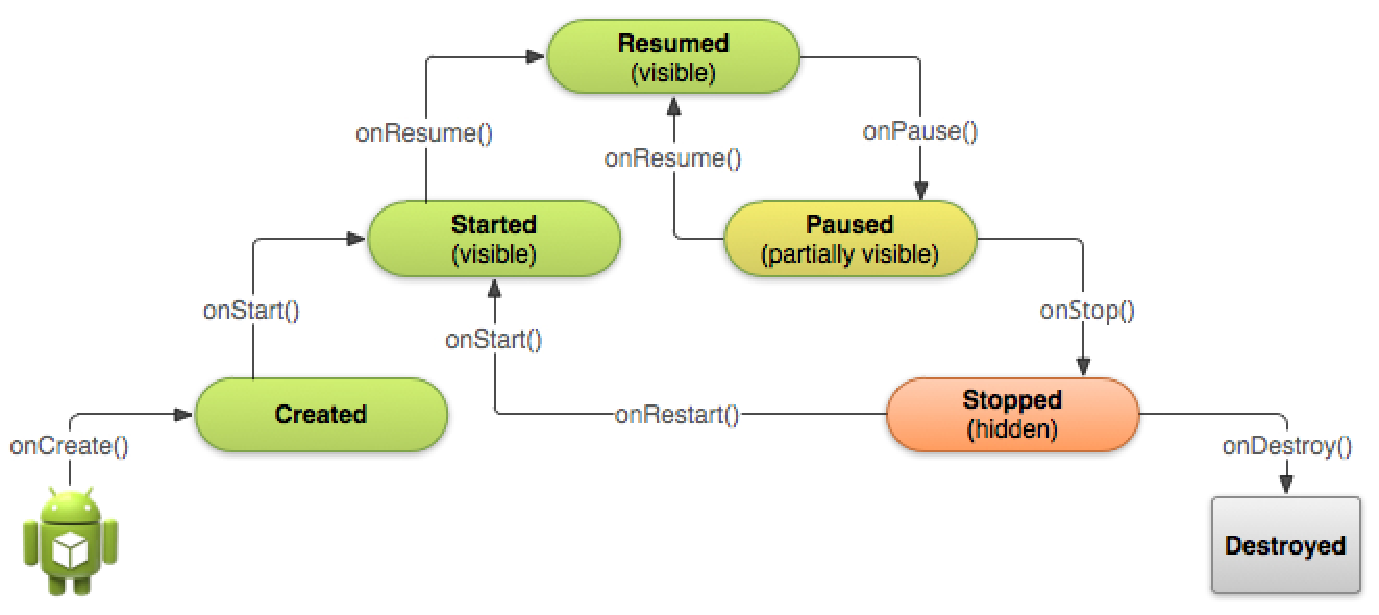
\includegraphics[width=0.90\textwidth]{./Imagenes/Vectorial/lifecycle-states.pdf}
    \caption{Estados de las aplicaciones Android}
\label{Fig:estados}
\end{figure}

La mayor\'ia de las aplicaciones contienen varias pantallas, lo cual significa que contienen varias actividades. Este concepto se pondr\'a posteriormente de manifiesto ya que para el desarrollo de la aplicaci\'on han sido necesarias 2 Actividades.
Cuando un usuario navega por una aplicaci\'on, la cierra, la vuelve a abrir o la minimiza, las instancias de las Actividades de la aplicaci\'on pasan por una serie de estados de su ciclo de vida (figura \ref{Fig:estados}). Estos estados pueden tener comportamientos definidos por los desarrolladores de la aplicaci\'on. Esto permite tener un control sobre lo que ocurre en cada uno de los estados de la aplicaci\'on. Para navegar por las transiciones entre las etapas del ciclo de vida de una actividad, la clase Activity proporciona un conjunto b\'asico de seis devoluciones de llamadas: \textbf{onCreate(), onStart(), onResume(), onPause(), onStop() y onDestroy().} El sistema invoca cada una de estas devoluciones de llamada cuando una actividad entra en un nuevo estado.


\begin{figure}[h]

\centering
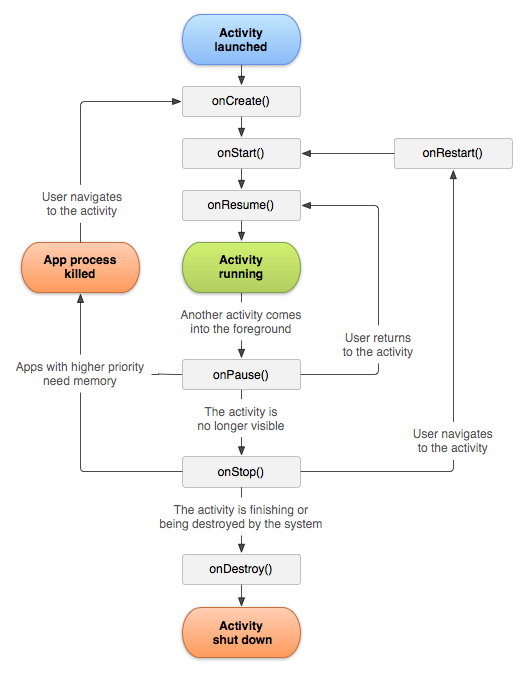
\includegraphics[width=0.7\textwidth]{./Imagenes/Bitmap/Ciclo_de_vida_Android}
\caption{Ciclo de vida de una Actividad de un sistema Android}
\end{figure}


Cada uno de los estados que tiene la actividad es llamado en un momento concreto de la ejecuci\'on de la Actividad. Las caracter\'isticas de cada uno de estos estados son las siguientes:

\begin {itemize}
\item \textbf{onCreate()} $\rightarrow$ Este m\'etodo es el primero que llama cuando se crea la Actividad. Este estado es utilizado para ejecutar la l\'ogica de la aplicaci\'on que debe ocurrir \'unicamente una vez en todo el ciclo de vida. Este m\'etodo recibe el par\'ametro \textit{\textbf{savedInstanceState}}, que es un objeto de tipo \textbf{\textit{Bundle}} que contiene el estado ya guardado de la actividad. Si la actividad nunca existi\'o, el valor del objeto \textit{Bundle} es nulo.
\item \textbf{onStart()} $\rightarrow$ Cuando la actividad entra en el estado Started, el sistema invoca esta devoluci\'on de llamada. La llamada \textit{onStart()} hace que el usuario pueda ver la actividad mientras la app se prepara para que esta entre en primer plano y se convierta en interactiva.
\item \textbf{onResume()} $\rightarrow$  La aplicaci\'on permanece en el estado \textit{} hasta que ocurre alg\'un evento que la quita de foco. Tal evento podr\'ia ser, por ejemplo, recibir una llamada telef\'onica, que el usuario navegue a otra actividad o que se apague la pantalla del dispositivo.
\item \textbf{onPause()} $\rightarrow$ Este estado se utiliza cuando se ha perdido el foco de una aplicaci\'on. Sin embargo una actividad con el estado Paused puede ser completamente visible si est\'a en el modo multiventana. En este estado no deben guardarse datos de la aplicaci\'on ya que es un estado que dura poco tiempo.
\item \textbf{onStop()} $\rightarrow$ En este estado es donde los componentes del ciclo de vida pueden detener cualquier funcionalidad que no necesite ejecutarse mientras el componente no sea visible en la pantalla. Este estado debe usarse para liberar o ajustar recursos que no son necesarios mientras no sea visible para el usuario.
\item \textbf{onDestroy()} $\rightarrow$ Se llama a este m\'etodo antes de que se finalice la actividad. El sistema invoca esta devoluci\'on de llamada cuando la aplicaci\'on se cierra. En este estado es donde los componentes del ciclo de vida pueden recuperar cualquier elemento que se necesite antes de que finalice la Actividad.
\end {itemize}

En el siguiente apartado se explicar\'a el uso de estas llamadas del sistema Android dentro del proyecto y la utilizaci\'on de diferentes actividades. Adem\'as se expondra la arquitectura de la aplicaci\'on desarrollada para Android.


%-------------------------------------------------------------------
\subsection {Desarrollo de la aplicaci\'on Android}
%-------------------------------------------------------------------

Una vez se tienen claras las diferentes llamadas que realiza el sistema Android y cu\'ando las realiza, es el momento de ver la aplicaci\'on que tienen en el desarrollo de este proyecto. Tal y como se plante\'o en la descripci\'on del protocolo de comunicaci\'on, la aplicaci\'on de Android necesita saber la IP y el puerto al que debe conectarse para enviar las pulsaciones. Para este primer paso se decidi\'o utilizar un c\'odigo QR que al leerlo con el m\'ovil, este contenga la direcci\'on IP y el puerto al que la aplicaci\'on se debe conectar. La lectura del c\'odigo QR y el env\'io de las puslaciones en pantalla son 2 procesos muy distintos e independientes, por esta raz\'on se implementaron 2 actividades diferentes.\\

La primera de estas actividades tiene como funci\'on activar la c\'amara del dispositivo Android para leer un c\'odigo QR. El contenido de este c\'odigo QR viene dado con el formato IP:Puerto (por ejemplo 192.168.1.1:5000). Una vez el c\'odigo QR es correcto, Android ofrece la posibilidad de lanzar una actividad nueva con una serie de par\'ametros. Para este proyecto uno de estos par\'ametros ser\'a el contenido del c\'odigo QR para que sea la actividad hija la que realice la conexi\'on y el intercambio de datos con el videojuego. \\

En esta segunda actividad se realiza la conexi\'on con el videojuego, lo que implica el env\'io de pulsaciones y la recepci\'on de im\'agenes y mensajes de vibraci\'on. Para que estos procesos se realicen de manera independiente y as\'incrona se han implementado 2 hilos de ejecuci\'on diferentes. Uno de ellos se encarga de gestionar la recepci\'on de datos y otro del env\'io de pulsaciones. Como esto debe realizarse al inicio de la ejecuci\'on de la activididad, el proceso de inicializaci\'on de estos hilos junto con los \textit{listeners} de las pulsaciones de la pantalla se realizan en el m\'etodo \textit{onCreate()}. \\

La actividad llamar\'a a la funci\'on \textit{onPause()} en caso de que se pierda el foco de la aplicaci\'on, es por eso que para parar por completo el consumo de la aplicaci\'on se cierran los hilos y se manda el mensaje de cierre de conexi\'on al juego. Esto ocurre para que no sea el sistema Android el que cierre los hilos de una manera inesperada.\\

Para que la aplicaci\'on Android cumpla los requisitos expuestos en el apartado de especificaci\'on del proyecto, se han implementado 4 clases:

\begin {itemize}
\item \textbf{MainActivity} $\rightarrow$ Esta primera clase corresponde a la primera actividad. En esta primera actividad se utiliza la c\'amara para leer un c\'odigo QR y guardar como par\'ametro el contenido del c\'odigo. Este contenido es la IP del equipo donde se est\'a ejecutando el juego y el puerto al que deben ser enviadas las pulsaciones del usuario. Estos datos son pasados a la actividad hija para comenzar a usar el m\'ovil como dispositivo de entrada.
\item \textbf{Controller} $\rightarrow$ Esta es la actividad principal. Desde esta actividad se recogen los datos de IP y puerto al que debe conectarse el dispositivo Android gracias a la lectura de un c\'odigo QR realizada con la actividad padre. Al crearse la actividad se lanza la ejecuci\'on de una hebra que se encargar\'a de recibir, leer e interpretar las im\'agenes que lleguen por red una vez la aplicaci\'on se conecte al juego. Desde esta clase se controla la pulsaci\'on del usuario en la pantalla. De esta pulsaci\'on se guardan 3 datos: posici\'on (x,y) donde se ha realizado la pulsaci\'on y el tipo de pulsaci\'on (presionar, levantar o arrastrar). Este dato permite soportar el \textit{multitouch} en la aplicaci\'on. El comportamiento de este hilo viene dado en la clase \textbf{UdpClientThread} que se encarga de preparar el datagrama de la pulsaci\'on y enviarlo. La \'ultima funci\'on de esta clase es la de cambiar la imagen que se muestra en la aplicaci\'on. 

\item \textbf{UdpClientThread} $\rightarrow$ Esta clase tiene como funci\'on el env\'io de datos a la aplicaci\'on donde se ejecuta el juego.Esta hebra se encarga del env\'io de paquetes que incluyen el tipo de pulsaci\'on que se ha realizado, la coordenada \textit{x} y la coordenada \textit{y} de la pantalla del dispositivo donde se ha realizado la pulsaci\'on. Una vez que la aplicaci\'on se cierre, el datagrama de cierre de conexi\'on se env\'ia desde esta hebra.

\item \textbf{Receive\_Image} $\rightarrow$ Esta clase se ejecuta desde una hebra distinta a la de la Actividad principal y la funci\'on que desempe\~na es la de recibir informaci\'on que mande el juego.En este hilo se espera la llegada del \textit{streaming} de im\'agenes desde el juevo. Estas im\'agenes se esperan en formato PNG ya que se realiza la descompresi\'on de este formato. El tiempo de vibraci\'on puede ser modificado en cualquier momento por el desarrollador por lo que ese mensaje tambi\'en es tratado en este hilo.
\end {itemize}


\begin{figure}[h]

\centering
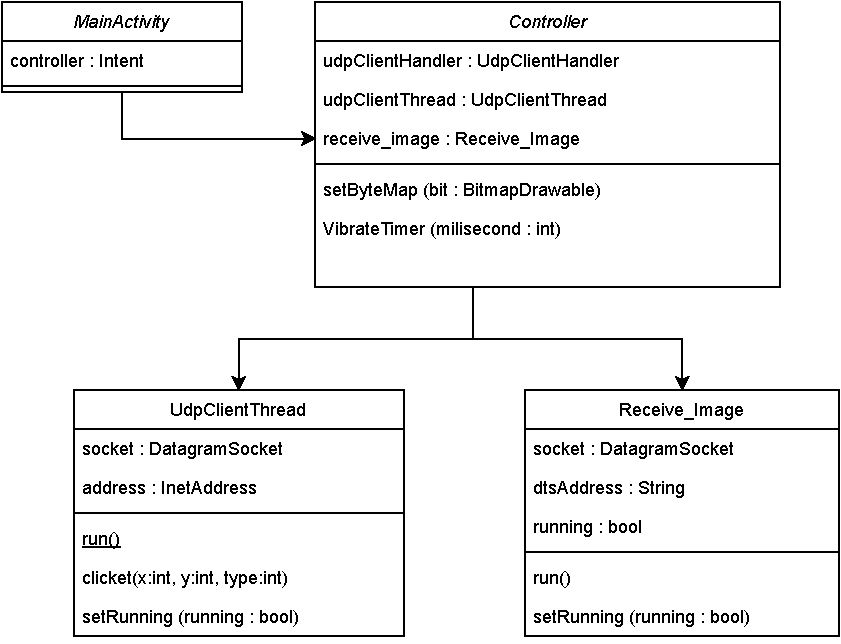
\includegraphics[width=0.9\textwidth]{./Imagenes/Vectorial/Arquitectura_App_Android.pdf}
\caption{Diagrama de clases de la aplicaci\'on Android}
\end{figure}

Se ha optado por una aplicaci\'on cerrada para que el desarrollador no tenga que implementar nueva funcionalidad en Android. El coste computacional de la aplicaci\'on es bajo, lo que permite ser utilizado en una gran cantidad de dispositivos. La divisi\'on en 2 actividades es debido a que el flujo de Android se basa en ir cambiando entre actividades para que cada una tenga un uso espec\'ifico. La primera actividad de usa para capturar un QR con la c\'amara y la segunda es utilizada para simular un mando.

%-------------------------------------------------------------------
\section{Implementaci\'on de la aplicaci\'on de Unity}
\label{unity}
%-------------------------------------------------------------------

Como se coment\'o al principio de este cap\'itulo, el motor de videojuegos elegido para la realizaci\'on de este proyecto ha sido Unity. Unity es un motor de videojuegos multiplataforma creado por \textit{Unity Technologies} en 2005. Unity est\'a disponible como plataforma de desarrollo para Microsoft, Mac OS y Linux y tiene soporte de compilaci\'on con m\'ultiples plataformas:

\begin {itemize}
\item \textbf{Web} $\rightarrow$ WebGL.
\item \textbf{PC} $\rightarrow$ Windows, SteamOS, Linux, OS X y Windows Store Apps.
\item \textbf{Dispositivos m\'oviles} $\rightarrow$ iOS, Android, Windows Phone.
\item \textbf{Smart TV} $\rightarrow$ tvOS, Samsung Smart TV, Android TV.
\item \textbf{Consolas} $\rightarrow$ PlayStation Vita, PlayStation 4, Xbox 360, Xbox One, Wii U, Nintendo 3DS, Nintendo Switch.
\item \textbf{Dispositivos de realidad virtual} $\rightarrow$ Oculus Rift, Google Cardboard, HTC Vive, PlayStation VR, Samsung Gear VR
\end {itemize}

Actualmente en la versi\'on 2021.1 de la documentaci\'on de Unity, no existe soporte para la nueva generaci\'on de consolas.\\


%-------------------------------------------------------------------
\subsection {Funcionamiento de Unity}
%-------------------------------------------------------------------

Unity es un motor de videojuegos que aglutina una gran variedad de herramientas para el desarrollo. Estas herramientas van desde inclusiones de \textbf{Scripts} para dar comportamientos espec\'ificos a cada una de las \textbf{Entidades} del juego hasta elementos m\'as visuales como diagramas de estado para el control de las animaciones de un modelo. Para que todos estos sistemas tan diferentes puedan convivir, hay una serie de funciones que se ejecutan en un orden determinado. Unity a su vez se compone de varios elementos clave:

\begin {itemize}
\item \textbf{Escena} $\rightarrow$  Las escenas contienen los objetos del juego. Pueden usarse para crear niveles, men\'us o cualquier estado del juego.
\item \textbf{GameObjects / Entidades} $\rightarrow$ Cada una de las escenas contiene objetos. Estos objetos se llaman GameObjects. Cualquier elemento es considerado un GameObject, no tiene por qu\'e tener una representaci\'on visual (m\'usica, c\'amara, etc).
\item \textbf{Componentes} $\rightarrow$ Los componentes son los diferentes atributos que se le dan a los GameObjects para que tengan funcionalidad (movimiento, posici\'on, animaci\'on, colisi\'on f\'isica, etc).
\end {itemize}

Unity ofrece una serie de componentes que dan una funcionalidad ya definida a un objeto, esta funcionalidad va desde tener una posici\'on definida en el mundo hasta emitir un sonido y realizar una animaci\'on. Los desarrolladores pueden desarrollar sus propios componentes usando Scipts. Estos scripts indican a las diferentes entidades c\'omo comportarse. El lenguaje seleccionado para este sistema de \textit{scripting} es C\# y un script debe estar vinculado a una entidad para que este se ejecute. \\

%-------------------------------------------------------------------
\subsection {Desarrollo de la API en Unity}
%-------------------------------------------------------------------

Las caracter\'isticas espec\'ificas de Unity deben tenerse en cuenta para la integraci\'on de la librer\'ia dentro del motor pero la librer\'ia est\'a desarrollada en .NET. El inicio de la comunicaci\'on entre en juego y  el m\'ovil se realiza con la lectura de un QR que lleva los datos de IP del PC donde se est\'a ejecutando el juego y el puerto donde el juego va a estar escuchando y por donde llegar\'an los datos del m\'ovil. Para conseguir que el m\'ovil disponga de estos datos se ha decidido utilizar un c\'odigo QR. Este c\'odigo se genera utilizando la librer\'ia \textbf{ZXing}\footnote{https://archive.codeplex.com/?p=zxingnet} en su versi\'on de .NET. \\

Para que la aplicaci\'on desarrollada en Unity cumpla los requisitos expuestos en el apartado de especificaci\'on del proyecto, se han realizado 2 clases:

\begin {itemize}
\item \textbf{UDPSocket} $\rightarrow$ Esta clase se utiliza para la creaci\'on de todo lo necesario para hacer funcionar esta herramienta. Con el m\'etodo \textbf{init()} se inician 2 hebras de ejecuci\'on diferentes. Una de ellas se encarga de enviar los datos necesarios al m\'ovil. Estos datos son tanto la vibraci\'on como la imagen a renderizar en el dispositivo o los mensajes de tipo \textit{keepalive} en caso de que el usuario no interactue con el juego en un tiempo determinado. La otra se encarga de recibir los datos de entrada del dispositivo y avisar a los diferentes \textit{listeners}. Estos listeners utilizan esa informaci\'on para los prop\'ositos desigandos por el desarrollador del juego (mover al personaje, pausar el juego, salir, etc). Esta clase tambi\'en se encarga de cerrar la conexi\'on.

\item \textbf{InputMobileInterface} $\rightarrow$ Esta interfaz permite al desarrollador del juego recibir los eventos que llegan desde el m\'ovil. Estos eventos son las coordenadas de las pulsaciones, las dimensiones del m\'ovil y el aviso del cierre de la conexi\'on por parte del m\'ovil. El m\'etodo \textbf{EndOfConnection()} comunica la p\'erdida de conexi\'on al \textit{listener} para que el usuario de la librer\'ia realice una acci\'on, por ejemplo pausar el juego hasta que la conexi\'on vuelva a iniciarse.
\end {itemize}

\begin{figure}[h]

\centering
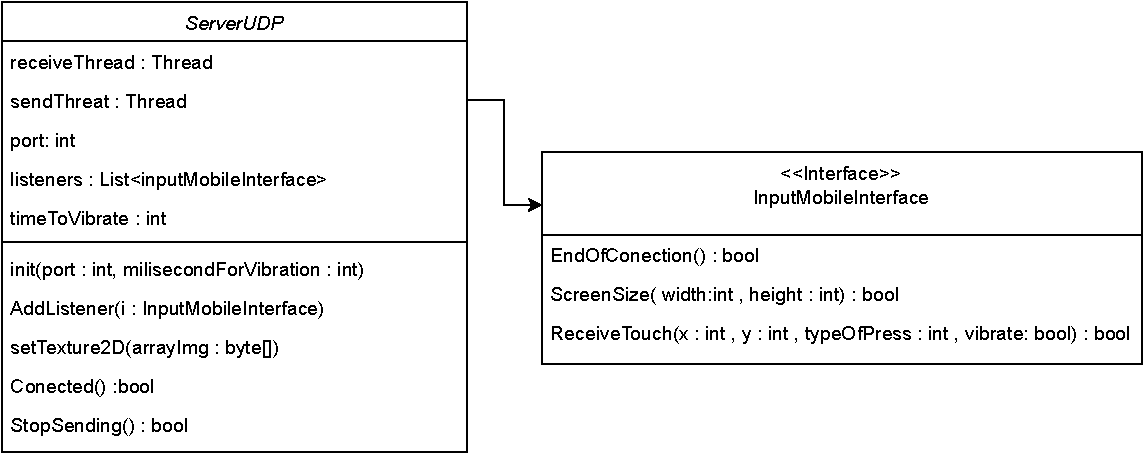
\includegraphics[width=0.9\textwidth]{./Imagenes/Vectorial/Arquitectura Unity.pdf}
\caption{Diagrama de clases de la aplicaci\'on de Unity}
\end{figure}

En este cap\'itulo se ha expuesto el desarrollo de las aplicaciones de Android y Unity. Adem\'as se han explicado algunos de los conocimientos b\'asicos para usar ambas herramientas. En el pr\'oximo cap\'itulo se explicar\'a la integraci\'on de la librer\'ia en un juego ya terminado con el que se realizar\'an una serie de pruebas con usuarios. Estas pruebas servir\'an para obtener datos del rendimiento del proyecto. Aplicando una serie de baremos se determinar\'a si el uso de la librer\'ia desarrollada cumple con las espectativas.\\

% Variable local para emacs, para  que encuentre el fichero maestro de
% compilaci�n y funcionen mejor algunas teclas r�pidas de AucTeX
%%%
%%% Local Variables:
%%% mode: latex
%%% TeX-master: "../ManualTeXiS.tex"
%%% End:


%---------------------------------------------------------------------
%
%                          Cap�tulo 5
%
%---------------------------------------------------------------------
%
% 05Bibliografia.tex
% Copyright 2009 Marco Antonio Gomez-Martin, Pedro Pablo Gomez-Martin
%
% This file belongs to the TeXiS manual, a LaTeX template for writting
% Thesis and other documents. The complete last TeXiS package can
% be obtained from http://gaia.fdi.ucm.es/projects/texis/
%
% Although the TeXiS template itself is distributed under the 
% conditions of the LaTeX Project Public License
% (http://www.latex-project.org/lppl.txt), the manual content
% uses the CC-BY-SA license that stays that you are free:
%
%    - to share & to copy, distribute and transmit the work
%    - to remix and to adapt the work
%
% under the following conditions:
%
%    - Attribution: you must attribute the work in the manner
%      specified by the author or licensor (but not in any way that
%      suggests that they endorse you or your use of the work).
%    - Share Alike: if you alter, transform, or build upon this
%      work, you may distribute the resulting work only under the
%      same, similar or a compatible license.
%
% The complete license is available in
% http://creativecommons.org/licenses/by-sa/3.0/legalcode
%
%---------------------------------------------------------------------

\chapter{Pruebas con usuarios}
\label{cap5}
\label{cap:pruebas}




% Variable local para emacs, para  que encuentre el fichero maestro de
% compilaci�n y funcionen mejor algunas teclas r�pidas de AucTeX
%%%
%%% Local Variables:
%%% mode: latex
%%% TeX-master: "../ManualTeXiS.tex"
%%% End:


\chapter{Conclusiones y trabajo futuro}
\label{cap7}
\label{cap:conclusiones}


El objetivo de este proyecto era el de utilizar un dispositivo m\'ovil como dispositivo de entrada para videojuegos. Para conseguir esto, se ha realizado una librer\'ia aplicable en el motor de videojuegos Unity con el objetivo de poder utilizar un dispositivo m\'ovil como dispositivo de entrada durante una sesi\'on de juego. Posterior al desarrollo de la librer\'ia, se ha ralizado una implementaci\'on en un juego con la que realizar pruebas de rendimiento de la herramienta.\\

El resultado de estas pruebas mostraron que la librer\'ia se comporta como se esperaba y que alcanza la tasa de fotogramas por segundo m\'inima aceptable en diferentes dispositivos. Estos resultados dejaron claro que el rendimiento de la librer\'ia est\'a ligado al \textit{hardware} donde se est\'a ejecutando. Adem\'as, las pruebas demuestran que las ejecuciones en los dispositivos Android en los que se han realizado las pruebas mantienen una estabilidad en el n\'umero de fotogramas por segundo a los que se ejecuta la aplicaci\'on.\\

En la parte de Unity se ha podido apreciar una velocidad de compresi\'on de im\'agenes baja, lo que lastra el rendimiento de la herramienta en sistemas con bajos recursos. En los sistemas en los que se ha probado a ejecutar la herramienta se ha podido ver que la tasa de fotogramas por segundo alcanza los l\'imites aceptados por la industria, 30 fotogramas por segundo. Optar por un modelo de librer\'ia vers\'atil para el desarrollador hace que recaiga toda la responsabilidad de optimizaci\'on del juego y de compresi\'on de im\'agenes en el desarrollador del juego.\\

\section{Trabajo futuro}

A pesar de alcanzar los m\'inimos aceptados por la industria en las ejecuciones realizadas, la herramienta muestra sus debilidades en sistemas con pocos recursos. Ya que estas mejoras no han podido entrar en el tiempo dedicado a la elaboraci\'on de este TFG, se van a proponer como trabajo futuro.\\

Existen diferentes algoritmos de compresi\'on de im\'agenes y en este proyecto se ha utilizado PNG debido a que se encuentra integrado en las dos plataformas utilizadas durante el desarrollo de la librer\'ia. Este formato de compresi\'on de im\'agenes es m\'as r\'apido cuanto menor sea la variedad de colores que contenga la im\'agen. En el videojuego utilizado para la prueba con usuarios, la im\'agen que se enviaba al dispositivo m\'ovil ten\'ia siempre los mismos colores, es por esto que el uso del formato PNG era suficiente. Para conseguir que los resultados sean mejores con im\'agenes m\'as complejas, se propone la b\'usqueda de un m\'etodo de compresi\'on de im\'agenes alternativo. En caso de decidir que el formato PNG es suficiente, se propone indagar m\'as sobre las posibilidades que ofrece este formato para ser comprimido. Alterar los par\'ametros de compresi\'on ayudar\'ia a que la herramienta fuese a una velocidad mayor y no se perdiese tanto tiempo en realizar la compresi\'on por defecto que ofrece Unity.\\

El uso de un m\'ovil como dispositivo de entrada no solo aporta una pantalla t\'actil en la que poder tener un mando, adem\'as de esto pueden utilizarse los diferentes sensores con los que cuentan estos dispositivos. Los sensores a los que se quiere dar m\'as importancia en este proyecto son el aceler\'ometro y el giroscopio. Estos sensores no se encuentran \'unicamente en los m\'oviles sino que tambi\'en se encuentran en otros dispositivos de entrada de algunas consolas. Por falta de tiempo, no se pudo implementar la monitorizaci\'on de estos sensores para ser utilizados en la librer\'ia pero su inclusi\'on dar\'ia m\'as versatilidad al desarrollador.\\

Por falta de tiempo durante el desarrollo de este trabajo, se abandon\'o la idea de permitir el uso de m\'ultiples m\'oviles durante una misma ejecuci\'on. Los juegos multijugador locales permitir\'ian exprimir al m\'aximo el uso de varios dispositivos m\'oviles, tal y como se hace en la saga de juegos PlayLink. Para conseguir esto es necesario la modificaci\'on del servidor de Unity para soportar m\'as de un cliente. \\

Adem\'as de lo relacionado con el apartado t\'ecnico del proyecto, un punto destacable a mejorar es el n\'umero de usuarios utilizado para las pruebas. Debido a la situaci\'on actual, las pruebas han tenido que realizarse en remoto, lo que hace que se necesite mucho m\'as tiempo para cada una de las pruebas. Con un cuestionario m\'as extenso y un n\'umero de usuarios mayor se podr\'ian dar valores estad\'isticos m\'as precisos. Con ello podr\'ian sacarse conclusiones con un peso estad\'istico mayor y tener una visi\'on m\'as global del rendimiento de la librer\'ia.

\chapter{Conclusions}
\label{cap7}
\label{cap:conclusions}


\section{Future Work}


\chapter{Trabajo Individual}
\label{cap7}
\label{cap:individual}

En esta secci\'on se exponen cu\'ales han sido las contribuciones de cada uno de los miembros del equipo al proyecto.\\



%-------------------------------------------------------------------
\section{Pablo G\'omez Calvo}
%-------------------------------------------------------------------

Al tratarse de un proyecto grande, la colaboraci\'on que hemos tenido que tener ambos integrantes del grupo ha sido muy relevante para el desarrollo del proyecto. Desde que comenz\'o el proyecto hemos realizado reuniones pr\'acticamente diarias para mantenernos informados sobre la tarea que estaba realizando cada uno. \\

En los primeros momentos del desarrollo del trabajo se decidi\'o que la metodolog\'ia que se iba a utilizar era SCRUM. El uso de esta metodolog\'ia \'agil hizo que durante los primeros pasos, un integrante del grupo se ocupase de la gesti\'on. Esa tarea fue llevada a cabo por mi. Esta tarea inclu\'ia la creaci\'on y gesti\'on del software de administraci\'on de proyectos, \textit{Pivotal Tracker}.\\

En los primeros momentos del desarrollo del trabajo asum\'i la parte de gesti\'on de reuniones, creaci\'on de los repositorios, b\'usqueda de plantillas de LaTeX y  b\'usqueda de documentaci\'on que se iba necesitando en los primeros prototipos. Tambi\'en la creaci\'on de una secci\'on donde se iban almacenando enlaces de libros interesantes, revistas, \textit{papers} y todo tipo de material relacionado con el TFG.\\

Una vez que ya se ten\'ian decididos los objetivos del proyecto, realiz\'abamos sesiones de trabajo conjunto en las que se realizaron varias pruebas de concepto para mostrar a los directores del TFG. Estas pruebas de concepto formaban parte de los hitos marcados y ten\'ian como prop\'osito tener siempre una versi\'on minimamente funcional del proyecto, tal y como plasman los fundamentos de SCRUM.\\

Los prototipos en los que particip\'e fueron los siguientes:

\begin{itemize}
  \item  Implementaci\'on de la librer\'ia ZXing en Unity.
  \item Cambio de actividades en Android.
\item Lectura de un c\'odigo QR.
\item Creaci\'on de un c\'odigo QR en Unity.
\item Creaci\'on de un servidor en Unity.
\item Comunicaci\'on entre un videojuego en Unity y una aplicaci\'on Android.
\end{itemize}

A la vez que se realizaban los prototipos se utilizaban las reuniones con los directores para debatir si las funcionalidades del proyecto eran las deseadas, o si por el contrario se necesitaba hacer una revisi\'on de las funcionalidades que se le quer\'ia dar al usuario de la librer\'ia. Estas diferentes versiones del proyecto fueron, en su mayor\'ia, desarrolladas en conjunto.\\

Una vez se decidieron las funcionalidades finales que deb\'ia de tener la librer\'ia, Sergio fue el encargado de realizar la implementaci\'on final de la herramienta mientras yo me dedicaba a la redacci\'on de la memoria. Mientras la parte de redacci\'on se iba desarrollando, ambos integrantes del grupo manten\'iamos las reuniones diarias junto con un abundante n\'umero de sesiones de trabajo conjunto. En estas sesiones se pon\'ian de manifiesto los avances en la implementaci\'on de la librer\'ia para poder plasmarlos en la memoria.\\

Con el desarrollo de la librer\'ia terminado, se realizaron sesiones conjuntas para revisar las partes ya escritas y realizar las correcciones aportadas por los profesores. En paralelo a esto, se repartieron de manera equitativa las pruebas con usuarios a realizar. En sesiones conjuntas posteriores se juntaron los datos, se analizaron y fueron plasmados en la memoria.\\

Al terminar todo lo relacionado con el c\'odigo y con el proyecto, las siguientes sesiones de trabajo conjunto se dedicaron a la correci\'on de bugs y a la revisi\'on de la memoria en busca de erratas. Mientras se realizaba esta \'ultima parte, tambi\'en se mantuvieron varias sesiones con los directores del proyecto en las que se corrigieron los errores encontrados en la estructura y redacci\'on de la memoria.


%-------------------------------------------------------------------
\section{Sergio Juan Higuera Velasco}
%-------------------------------------------------------------------

Trat\'andose de un proyecto grande realizado entre dos personas y conociendo las din\'amicas de grupo gracias a proyectos anteriores, se decidi\'o que gran parte del tiempo dedicado a este proyecto iba a ser en sesiones conjuntas de trabajo. Al inicio del proyecto se realizaron sesiones conjuntas en las que buscar informaci\'on, buscar repositorios y decidir las herramientas que se iban a utilizar. Las tareas a realizar se iban almacenando en el \textit{dashboard} de tareas pendientes y se iban realizando por orden de prioridad.\\

Durante las primeras fases del proyecto se buscar\'o todo tipo de informaci\'on relacionada con el tema tratado en el TFG, con esto se pretend\'ia crear una peque\~na bibliograf\'ia con la que poder desarrollar el trabajo. Una de las primeras labores que tuvimos que desempe\~nar fue la de la b\'usqueda de libros, conferencias, art\'iculos y \textit{papers} de los temas tratados en este TFG.\\

Junto con la b\'usqueda de informaci\'on, las primeras fases del desarrollo se utilizaron para desarrollar muchos prototipos con los que experimentar las diferentes funcionalidades que se quer\'ian a\~nadir al proyecto final. Estos prototipos se realizaron en su mayor\'ia en sesiones de trabajo conjuntas. En estas sesiones conjuntas se aprovechaba para intercambiar ideas y proponer el uso de las diferentes herramientas disponibles. \\

Los prototipos en los que particip\'e fueron los siguientes:

\begin{itemize}
  \item  Cambio de actividades en Android.
  \item Comunicaci\'on entre ambos dispositivos.
\item Defininici\'on he implementaci\'on de los diferentes datagramas del protocolo de comunicaci\'on.
\item Creaci\'on de un c\'odigo QR en Unity.
\item Creaci\'on de un servidor en Unity.
\item Manejo de varios hilos concurrentes en Unity.
\item Manejo de varios hilos concurrentes en Android.
\end{itemize}

Mientras mi compa\~nero se orientaba m\'as a la b\'usqueda de informaci\'on, at\'iculos y libros relacionados con el proyecto, la labor que asum\'i fue la de investigaci\'on y aprendizaje de las diferentes herramientas que se han utilizado en la realizaci\'on de este TFG. Entre estas tareas se encuentra la de la realizaci\'on de una parte de las pruebas de concepto que se fueron realizando a lo largo del tiempo que ha durado este proyecto. Al ser conocedor de las herramientas, la parte de documentaci\'on sobre estas herramientas como Unity o Android fueron responsabilidad mia.\\

En la parte de redacci\'on la memoria, los cap\'itulos en los que m\'as he estado involucrado han sido el 3, 4 y 5. Esto se debe a que en estos cap\'itulos se explicaba todo el trabajo de desarrollo de prototipos, la posterior creaci\'on del protocolo y la implementaci\'on de la librer\'ia.

Una vez se decidieron los objetivos finales del trabajo, Pablo y yo nos dividimos un poco m\'as para poder avanzar en paralelo. Durante las sesiones de trabajo conjunto se explicaban los avances en la implementaci\'on de la librer\'ia para que mi compa\~nero pudiera plasmarlos en esta memoria. Esta fue la din\'amica que se sigui\'o hasta la realizaci\'on de las pruebas con usuarios.\\

Para las pruebas con usuarios era necesario buscar un proyecto en el que incluir la librer\'ia. Mi labor en esta parte fue la de incluir la librer\'ia en un proyecto y prepararlo para realizar una prueba de rendimiento con usuarios. Para conseguir esto implement\'e un \textit{tracker} con el que medir el rendimiento de los procesos principales de la librer\'ia. La realziaci\'on de las pruebas se repartieron a partes iguales y en sesiones posteriores se realiz\'o el an\'alisis. \\

Para el an\'alisis de los datos de las pruebas y poder sacar las gr\'aficas que se encuentran en el cap\'itulo 5, implement\'e en \textit{python} un \textit{script} con el que poder realizar el tratamiento de los datos obtenidos.\\

Como aportaci\'on final, realic\'e los siguientes  puntos de la memoria:
\begin{itemize}
  \item  Redacci\'on del ``Abstract''.
  \item Redacci\'on del cap\'itulo 1 en ingl\'es.
\item Redacci\'on de la secci\'on 6.1 ``Trabajo futuro''.
\item Redacci\'on del cap\'itulo 7.
\item B\'usqueda de im\'agenes y referencias para el cap\'itulo 2.
\end{itemize}


% Ap�ndices
%\appendix
%%---------------------------------------------------------------------
%
%                          Parte 3
%
%---------------------------------------------------------------------
%
% Parte3.tex
% Copyright 2009 Marco Antonio Gomez-Martin, Pedro Pablo Gomez-Martin
%
% This file belongs to the TeXiS manual, a LaTeX template for writting
% Thesis and other documents. The complete last TeXiS package can
% be obtained from http://gaia.fdi.ucm.es/projects/texis/
%
% Although the TeXiS template itself is distributed under the 
% conditions of the LaTeX Project Public License
% (http://www.latex-project.org/lppl.txt), the manual content
% uses the CC-BY-SA license that stays that you are free:
%
%    - to share & to copy, distribute and transmit the work
%    - to remix and to adapt the work
%
% under the following conditions:
%
%    - Attribution: you must attribute the work in the manner
%      specified by the author or licensor (but not in any way that
%      suggests that they endorse you or your use of the work).
%    - Share Alike: if you alter, transform, or build upon this
%      work, you may distribute the resulting work only under the
%      same, similar or a compatible license.
%
% The complete license is available in
% http://creativecommons.org/licenses/by-sa/3.0/legalcode
%
%---------------------------------------------------------------------

% Definici�n de la �ltima parte del manual, los ap�ndices

\partTitle{Ap�ndices}

\makepart

%%---------------------------------------------------------------------
%
%                          Ap�ndice 1
%
%---------------------------------------------------------------------
%
% 01AsiSeHizo.tex
% Copyright 2009 Marco Antonio Gomez-Martin, Pedro Pablo Gomez-Martin
%
% This file belongs to the TeXiS manual, a LaTeX template for writting
% Thesis and other documents. The complete last TeXiS package can
% be obtained from http://gaia.fdi.ucm.es/projects/texis/
%
% Although the TeXiS template itself is distributed under the 
% conditions of the LaTeX Project Public License
% (http://www.latex-project.org/lppl.txt), the manual content
% uses the CC-BY-SA license that stays that you are free:
%
%    - to share & to copy, distribute and transmit the work
%    - to remix and to adapt the work
%
% under the following conditions:
%
%    - Attribution: you must attribute the work in the manner
%      specified by the author or licensor (but not in any way that
%      suggests that they endorse you or your use of the work).
%    - Share Alike: if you alter, transform, or build upon this
%      work, you may distribute the resulting work only under the
%      same, similar or a compatible license.
%
% The complete license is available in
% http://creativecommons.org/licenses/by-sa/3.0/legalcode
%
%---------------------------------------------------------------------

\chapter{As� se hizo...}
\label{ap1:AsiSeHizo}

\begin{FraseCelebre}
\begin{Frase}
Pones tu pie en el camino y si no cuidas tus pasos, nunca sabes a donde te pueden llevar.
\end{Frase}
\begin{Fuente}
John Ronald Reuel Tolkien, El Se�or de los Anillos
\end{Fuente}
\end{FraseCelebre}

\begin{resumen}
Este ap�ndice cuenta algunos aspectos pr�cticos que nos planteamos en
su momento durante la redacci�n de la tesis (a modo de ``as� se hizo
nuestra tesis''). En realidad no es m�s que una excusa para que �ste
manual tenga un ap�ndice que sirva de ejemplo en la plantilla.
\end{resumen}

%-------------------------------------------------------------------
\section{Edici�n}
%-------------------------------------------------------------------
\label{ap1:edicion}

Ya indicamos en la secci�n~\ref{cap3:sec:editores} (p�gina
\pageref{cap3:sec:editores}) que \texis\ est� preparada para
integrarse bien con emacs, en particular con el modo Auc\TeX.

Eso era en realidad un s�ntoma indicativo de que en nuestro trabajo
cotidiano utilizamos emacs para editar ficheros \LaTeX. Es cierto que
inicialmente utilizamos otros editores creados expresamente para la
edici�n de ficheros en \LaTeX, pero descubrimos emacs y ha llegado
para quedarse (la figura~\ref{cap3:fig:emacs} mostraba una captura del
mismo mientras cre�bamos este manual). Ten en cuenta que si utilizas
Windows, tambi�n puedes usar emacs para editar; no lo consideres como
algo que s�lo se utiliza en el mundo Unix. Nosotros lo usamos a diario
tanto en Linux como en Windows.

No obstante, hay que reconocer que emacs \emph{no} es f�cil de
utilizar al principio (el manual de referencia de \cite{emacsStallman}
tiene m�s de 550 p�ginas); su curva de aprendizaje es empinada,
especialmente si quieres sacarle el m�ximo partido, o al menos
beneficiarte de algunas de sus combinaciones de teclas. Pero una vez
que consigues \emph{no} mover las manos para desplazar el cursor sobre
el documento, manejas las teclas r�pidas para a�adir los comandos
\LaTeX\ m�s utilizados y conoces las combinaciones de Auc\TeX\ para
moverte por el documento o buscar las entradas de la bibliograf�a, no
cambiar�s f�cilmente a otro editor.

Si quieres aprovechar emacs, no debes dejar de leer el documento que
nos introdujo a nosotros en el modo Auc\TeX, ``\emph{Creaci�n de
  ficheros \LaTeX\ con GNU Emacs}'' \citep{AtazLopezEmacs}.

%-------------------------------------------------------------------
\section{Encuadernaci�n}
%-------------------------------------------------------------------
\label{ap1:encuadernacion}

Si has mirado con un poco de atenci�n este manual, habr�s visto que
los m�rgenes que tiene son bastante grandes. \texis\ no configura
los m�rgenes a unos valores concretos sino que, directamente, utiliza
los que se establecen por defecto en la clase \texttt{book} de \LaTeX.

Aunque es m�s o menos reconocido que si \LaTeX\ utiliza esos m�rgenes
debe tener una raz�n de peso (y de hecho la tiene, se utilizan esos
para que el n�mero de letras por l�nea sea el id�neo para su lectura),
cuando se comienza a mirar el documento con los ojos del que quiere
verlo encuadernado, es cierto que parecen excesivos. Y empiezas a
abrir libros, regla en mano, para medir qu� m�rgenes utilizan. Y
reconoces que son mucho m�s peque�os (y razonables) que el de tu
maravilloso escrito. Al menos ese fue nuestro caso.

En ese momento, una soluci�n es \emph{reducir} esos m�rgenes para que
aquello quede mejor. Sin embargo nuestra opci�n no fue esa. Si tu
situaci�n te permite \emph{no} encuadernar el documento en formato
DIN-A4, entonces puedes ir a la reprograf�a de turno y pedir que, una
vez impreso, te guillotinen esos m�rgenes.

Tu escrito quedar� entonces en ``formato libro'', mucho m�s manejable
que el gran DIN-A4, y con unos m�rgenes mucho m�s razonables. La
figura~\ref{ap1:fig:encuadernacion} muestra el resultado, comparando
el tama�o final con el de un folio, que aparece superpuesto.

\figura{Bitmap/0A/encuadernacion}{width=0.7\textwidth}%
       {ap1:fig:encuadernacion}{Encuadernaci�n y m�rgenes guillotinados}

%-------------------------------------------------------------------
\section{En el d�a a d�a}
%-------------------------------------------------------------------
\label{ap1:cc}

Para terminar este breve ap�ndice, describimos ahora un modo de
trabajo que, si bien no utilizamos en su d�a para la escritura de la
tesis, s� hemos utilizado desde hace alg�n tiempo para el resto de
nuestros escritos de \LaTeX , incluidos \texis\ y �ste, su manual.

Estamos hablando de lo que se conoce en el mundo de la ingenier�a del
software como \emph{integraci�n cont�nua} \citep{Fowler06}. En
concreto, la integraci�n cont�nua consiste en aprovecharse del
servidor del control de versiones para realizar, en cada
\emph{commit} o actualizaci�n realizada por los autores, una
comprobaci�n de si los ficheros que se han subido son de verdad
correctos.

En el mundo del desarrollo software donde un proyecto puede involucrar
decenas de personas realizando varias actualizaciones diarias, la
integraci�n cont�nua tiene mucha importancia. Despu�s de que un
programador realice una actualizaci�n, un servidor dedicado comprueba
que el proyecto sigue compilando correctamente (e incluso ejecuta los
test de unidad asociados). En caso de que la actualizaci�n haya
estropeado algo, el servidor de integraci�n env�a un mensaje de correo
electr�nico al autor de ese \emph{commit} para avisarle del error y
que �ste lo subsane lo antes posible, de forma que se perjudique lo
menos posible al resto de desarrolladores.

Esa misma idea la hemos utilizado en la elaboraci�n de \texis\ y
de este manual. Cada vez que uno de los autores sub�a al SVN alg�n
cambio, el servidor comprobaba que el fichero maestro segu�a siendo
correcto, es decir, que se pod�a generar el PDF final sin errores.

No entraremos en m�s detalles de c�mo hacer esto. El lector interesado
puede consultar \citet{CCLatex}. Como se explica en ese art�culo
algunas ventajas del uso de esta t�cnica son:

\begin{figure}[t]
  \centering
  %
  \subfloat[][P�gina de descarga del documento generado]{
     \includegraphics[width=0.445\textwidth]%
                     {Imagenes/Bitmap/0A/dashboard}
     \label{ap1:fig:dashboard}
  }
  \qquad
  \subfloat[][M�tricas del proyecto]{
     \includegraphics[width=0.445\textwidth]%
                     {Imagenes/Bitmap/0A/metrics}
     \label{ap1:fig:metrics}
  }
 \caption{Servidor de integraci�n cont�nua\label{ap1:fig:cc}}
\end{figure}

\begin{itemize}
\item Se tiene la seguridad de que la versi�n disponible en el control
  de versiones es v�lida, es decir, es capaz de generar sin errores el
  documento final.

\item Se puede configurar el servidor de integraci�n cont�nua para que
  cada vez que se realiza un \emph{commit}, env�e un mensaje de correo
  electr�nico \emph{a todos los autores} del mismo. De esta forma
  todos los colaboradores est�n al tanto del progreso del mismo.

\item Se puede configurar para que el servidor haga p�blico (via
  servidor Web) el PDF del documento (ver
  figura~\ref{ap1:fig:dashboard}). Esto es especialmente �til para
  revisores del texto como tutores de tesis, que no tendr�n que
  preocuparse de descargar y compilar los \texttt{.tex}.
\end{itemize}

Por �ltimo, el servidor tambi�n permite ver la evoluci�n del proyecto.
La figura~\ref{ap1:fig:metrics} muestra una gr�fica que el servidor de
integraci�n cont�nua muestra donde se puede ver la fecha (eje
horizontal) y hora (eje vertical) de cada \emph{commit} en el
servidor; los puntos rojos representan commits cuya compilaci�n fall�.



% Variable local para emacs, para  que encuentre el fichero maestro de
% compilaci�n y funcionen mejor algunas teclas r�pidas de AucTeX
%%%
%%% Local Variables:
%%% mode: latex
%%% TeX-master: "../ManualTeXiS.tex"
%%% End:


\backmatter

%
% Bibliograf�a
%

\bibliography{sample}

%
% �ndice de palabras
%

\ifx\generaindice\undefined
\else
%---------------------------------------------------------------------
%
%                        TeXiS_indice.tex
%
%---------------------------------------------------------------------
%
% TeXiS_indice.tex
% Copyright 2009 Marco Antonio Gomez-Martin, Pedro Pablo Gomez-Martin
%
% This file belongs to TeXiS, a LaTeX template for writting
% Thesis and other documents. The complete last TeXiS package can
% be obtained from http://gaia.fdi.ucm.es/projects/texis/
%
% This work may be distributed and/or modified under the
% conditions of the LaTeX Project Public License, either version 1.3
% of this license or (at your option) any later version.
% The latest version of this license is in
%   http://www.latex-project.org/lppl.txt
% and version 1.3 or later is part of all distributions of LaTeX
% version 2005/12/01 or later.
%
% This work has the LPPL maintenance status `maintained'.
% 
% The Current Maintainers of this work are Marco Antonio Gomez-Martin
% and Pedro Pablo Gomez-Martin
%
%---------------------------------------------------------------------
%
% Contiene  los  comandos  para  generar  el �ndice  de  palabras  del
% documento.
%
%---------------------------------------------------------------------
%
% NOTA IMPORTANTE: el  soporte en TeXiS para el  �ndice de palabras es
% embrionario, y  de hecho  ni siquiera se  describe en el  manual. Se
% proporciona  una infraestructura  b�sica (sin  terminar)  para ello,
% pero  no ha  sido usada  "en producci�n".  De hecho,  a pesar  de la
% existencia de  este fichero, *no* se incluye  en Tesis.tex. Consulta
% la documentaci�n en TeXiS_pream.tex para m�s informaci�n.
%
%---------------------------------------------------------------------


% Si se  va a generar  la tabla de  contenidos (el �ndice  habitual) y
% tambi�n vamos a  generar el �ndice de palabras  (ambas decisiones se
% toman en  funci�n de  la definici�n  o no de  un par  de constantes,
% puedes consultar modo.tex para m�s informaci�n), entonces metemos en
% la tabla de contenidos una  entrada para marcar la p�gina donde est�
% el �ndice de palabras.

\ifx\generatoc\undefined
\else
   \addcontentsline{toc}{chapter}{\indexname}
\fi

% Generamos el �ndice
\printindex

% Variable local para emacs, para  que encuentre el fichero maestro de
% compilaci�n y funcionen mejor algunas teclas r�pidas de AucTeX

%%%
%%% Local Variables:
%%% mode: latex
%%% TeX-master: "./tesis.tex"
%%% End:

\fi

%
% Lista de acr�nimos
%

% S�lo  lo  generamos  si  est� declarada  \generaacronimos.  Consulta
% TeXiS.sty para m�s informaci�n.


\ifx\generaacronimos\undefined
\else
%%---------------------------------------------------------------------
%
%                        TeXiS_acron.tex
%
%---------------------------------------------------------------------
%
% TeXiS_acron.tex
% Copyright 2009 Marco Antonio Gomez-Martin, Pedro Pablo Gomez-Martin
%
% This file belongs to TeXiS, a LaTeX template for writting
% Thesis and other documents. The complete last TeXiS package can
% be obtained from http://gaia.fdi.ucm.es/projects/texis/
%
% This work may be distributed and/or modified under the
% conditions of the LaTeX Project Public License, either version 1.3
% of this license or (at your option) any later version.
% The latest version of this license is in
%   http://www.latex-project.org/lppl.txt
% and version 1.3 or later is part of all distributions of LaTeX
% version 2005/12/01 or later.
%
% This work has the LPPL maintenance status `maintained'.
% 
% The Current Maintainers of this work are Marco Antonio Gomez-Martin
% and Pedro Pablo Gomez-Martin
%
%---------------------------------------------------------------------
%
% Contiene  los  comandos  para  generar  el listado de acr�nimos
% documento.
%
%---------------------------------------------------------------------
%
% NOTA IMPORTANTE:  para que la  generaci�n de acr�nimos  funcione, al
% menos  debe  existir  un  acr�nimo   en  el  documento.  Si  no,  la
% compilaci�n  del   fichero  LaTeX  falla  con   un  error  "extra�o"
% (indicando  que  quiz�  falte  un \item).   Consulta  el  comentario
% referente al paquete glosstex en TeXiS_pream.tex.
%
%---------------------------------------------------------------------


% Redefinimos a espa�ol  el t�tulo de la lista  de acr�nimos (Babel no
% lo hace por nosotros esta vez)

\def\listacronymname{Lista de acr�nimos}

% Para el glosario:
% \def\glosarryname{Glosario}

% Si se  va a generar  la tabla de  contenidos (el �ndice  habitual) y
% tambi�n vamos a  generar la lista de acr�nimos  (ambas decisiones se
% toman en  funci�n de  la definici�n  o no de  un par  de constantes,
% puedes consultar config.tex  para m�s informaci�n), entonces metemos
% en la  tabla de contenidos una  entrada para marcar  la p�gina donde
% est� el �ndice de palabras.

\ifx\generatoc\undefined
\else
   \addcontentsline{toc}{chapter}{\listacronymname}
\fi


% Generamos la lista de acr�nimos (en realidad el �ndice asociado a la
% lista "acr" de GlossTeX)

\printglosstex(acr)

% Variable local para emacs, para  que encuentre el fichero maestro de
% compilaci�n y funcionen mejor algunas teclas r�pidas de AucTeX

%%%
%%% Local Variables:
%%% mode: latex
%%% TeX-master: "../Tesis.tex"
%%% End:

\fi

%
% Final
%%
%%---------------------------------------------------------------------
%
%                      fin.tex
%
%---------------------------------------------------------------------
%
% fin.tex
% Copyright 2009 Marco Antonio Gomez-Martin, Pedro Pablo Gomez-Martin
%
% This file belongs to the TeXiS manual, a LaTeX template for writting
% Thesis and other documents. The complete last TeXiS package can
% be obtained from http://gaia.fdi.ucm.es/projects/texis/
%
% Although the TeXiS template itself is distributed under the 
% conditions of the LaTeX Project Public License
% (http://www.latex-project.org/lppl.txt), the manual content
% uses the CC-BY-SA license that stays that you are free:
%
%    - to share & to copy, distribute and transmit the work
%    - to remix and to adapt the work
%
% under the following conditions:
%
%    - Attribution: you must attribute the work in the manner
%      specified by the author or licensor (but not in any way that
%      suggests that they endorse you or your use of the work).
%    - Share Alike: if you alter, transform, or build upon this
%      work, you may distribute the resulting work only under the
%      same, similar or a compatible license.
%
% The complete license is available in
% http://creativecommons.org/licenses/by-sa/3.0/legalcode
%
%---------------------------------------------------------------------
%
% Contiene la �ltima p�gina
%
%---------------------------------------------------------------------


% Ponemos el marcador en el PDF al nivel adecuado, dependiendo
% de su hubo partes en el documento o no (si las hay, queremos
% que aparezca "al mismo nivel" que las partes.
\ifpdf
\ifx\tienePartesTeXiS\undefined
   \pdfbookmark[0]{Fin}{fin}
\else
   \pdfbookmark[-1]{Fin}{fin}
\fi
\fi

\thispagestyle{empty}\mbox{}

\vspace*{4cm}

\small

\hfill \emph{--�Qu� te parece desto, Sancho? -- Dijo Don Quijote --}

\hfill \emph{Bien podr�n los encantadores quitarme la ventura,}

\hfill \emph{pero el esfuerzo y el �nimo, ser� imposible.}

\hfill 

\hfill \emph{Segunda parte del Ingenioso Caballero} 

\hfill \emph{Don Quijote de la Mancha}

\hfill \emph{Miguel de Cervantes}

\vfill%space*{4cm}

\hfill \emph{--Buena est� -- dijo Sancho --; f�rmela vuestra merced.}

\hfill \emph{--No es menester firmarla -- dijo Don Quijote--,}

\hfill \emph{sino solamente poner mi r�brica.}

\hfill 

\hfill \emph{Primera parte del Ingenioso Caballero} 

\hfill \emph{Don Quijote de la Mancha}

\hfill \emph{Miguel de Cervantes}


\newpage
\thispagestyle{empty}\mbox{}

\newpage

% Variable local para emacs, para  que encuentre el fichero maestro de
% compilaci�n y funcionen mejor algunas teclas r�pidas de AucTeX

%%%
%%% Local Variables:
%%% mode: latex
%%% TeX-master: "../Tesis.tex"
%%% End:


\end{document}
